% =====================================================================
%  Báo cáo Bài tập lớn CO4031 - Kho dữ liệu và Hệ hỗ trợ Quyết định
%  Biên dịch: pdfLaTeX (Overleaf: Menu -> Compiler = pdfLaTeX), 2 lần để có mục lục.
%  Hình số liệu sinh lại bằng: python report/scripts/make_figures.py
% =====================================================================
\documentclass[a4paper,11pt]{article}
\usepackage[utf8]{inputenc}
\usepackage[T5]{fontenc}
\usepackage[english]{babel}
\usepackage[top=3cm, bottom=2.5cm, left=2.75cm, right=2.75cm, headheight=40pt]{geometry}
\renewcommand{\ttdefault}{pcr}   % chữ đơn cách kiểu Courier như template
\linespread{1.3}
\setlength{\parindent}{2em}
\usepackage{fancyhdr}
\usepackage{lastpage}
\usepackage{graphicx}
\usepackage{tabularx}
\usepackage{booktabs}
\usepackage{longtable}
\usepackage{multirow}
\usepackage[table]{xcolor}
\usepackage[nottoc]{tocbibind}
\usepackage{caption}
\usepackage{float}
\usepackage{amsmath}
\usepackage{enumitem}
\usepackage{listings}
\usepackage{tikz}
\usetikzlibrary{positioning,arrows.meta,shapes.multipart,fit,calc}
\usepackage{hyperref}
\hypersetup{colorlinks=true, linkcolor=black, urlcolor=blue, citecolor=black}

% Tên danh mục theo template Big Data (CO3137)
\addto\captionsenglish{\renewcommand{\contentsname}{Table of Contents}}

% Màu dùng trong sơ đồ TikZ và nhãn mức nhu cầu
\definecolor{primary}{HTML}{10B981}
\definecolor{heading1}{HTML}{1F4E79}
\definecolor{heading2}{HTML}{2E75B6}
\definecolor{heading3}{HTML}{376092}
\definecolor{lvlow}{HTML}{16A34A}
\definecolor{lvmed}{HTML}{F59E0B}
\definecolor{lvhigh}{HTML}{DC2626}
\definecolor{codebg}{gray}{0.94}

% Header và Footer theo template HCMUT (logo + tên trường; môn học + Page x/y)
\pagestyle{fancy}
\fancyhf{}
\fancyhead[L]{%
  \begin{tabular}{rl}
    \begin{picture}(25,15)(0,0)
      \put(0,-8){
\includegraphics[width=8mm, height=8mm]{figures/hcmut.png}}
    \end{picture} &
    \begin{tabular}{l}
      \textbf{\ttfamily HO CHI MINH CITY UNIVERSITY OF TECHNOLOGY - VNU-HCMC}\\
      \textbf{\ttfamily FACULTY OF COMPUTER SCIENCE AND ENGINEERING}
    \end{tabular}
  \end{tabular}}
\fancyfoot[L]{\scriptsize\ttfamily Data Warehouse and Decision Support System (CO4031) - 261}
\fancyfoot[R]{\scriptsize\ttfamily Page {\thepage}/\pageref{LastPage}}
\renewcommand{\headrulewidth}{0.3pt}
\renewcommand{\footrulewidth}{0.3pt}

% Đoạn mã: nền xám, khung mảnh, chú thích bên dưới (chỉ dùng ký tự ASCII trong mã nguồn)
\lstset{basicstyle=\ttfamily\scriptsize\linespread{1.1}\selectfont, backgroundcolor=\color{codebg}, frame=single,
  rulecolor=\color{gray!40}, breaklines=true, columns=fullflexible, captionpos=b,
  keywordstyle=\bfseries, showstringspaces=false, xleftmargin=2pt, xrightmargin=2pt}

% Tiện ích
\newcommand{\todo}[1]{\textcolor{red}{\textbf{[#1]}}}   % chỗ nhóm cần tự điền
\newcommand{\code}[1]{\texttt{#1}}
\newcommand{\lvl}[2]{\colorbox{#1}{\textcolor{white}{\footnotesize\textbf{#2}}}}
\newcommand{\Low}{\lvl{lvlow}{Thấp}}
\newcommand{\Med}{\lvl{lvmed}{Trung bình}}
\newcommand{\High}{\lvl{lvhigh}{Cao}}
\newcommand{\chap}[1]{\section{#1}}
\newcommand{\sect}[1]{\subsection{#1}}
\newcommand{\subsect}[1]{\subsubsection{#1}}
\setlist{itemsep=2pt, topsep=4pt}
\renewcommand{\arraystretch}{1.25}

% Thông tin chung - sửa tại đây
\newcommand{\repoURL}{\url{https://github.com/ball7905/Public-Bike-Sharing-}}
\newcommand{\videoURL}{\todo{Link video YouTube (unlisted) / Google Drive - nếu nhóm thuyết trình qua video}}

\begin{document}

% ==================== TRANG BÌA (theo template HCMUT / Big Data CO3137) ====================
\begin{titlepage}
\thispagestyle{empty}
\begin{tikzpicture}[remember picture, overlay]
  % khung ngoài mảnh và khung xanh đậm hai lớp
  \draw[gray!60, line width=0.4pt]
    ($(current page.north west)+(1.2cm,-1.2cm)$) rectangle ($(current page.south east)+(-1.2cm,1.2cm)$);
  \draw[blue!70!black, line width=3pt]
    ($(current page.north west)+(1.5cm,-1.5cm)$) rectangle ($(current page.south east)+(-1.5cm,1.5cm)$);
  \draw[blue!70!black, line width=0.8pt]
    ($(current page.north west)+(1.75cm,-1.75cm)$) rectangle ($(current page.south east)+(-1.75cm,1.75cm)$);
\end{tikzpicture}

\begin{center}
\linespread{1.15}\selectfont
\vspace*{1.2cm}
{\small\textbf{VIETNAM NATIONAL UNIVERSITY - HCMC}}\\
{\small\textbf{HO CHI MINH CITY UNIVERSITY OF TECHNOLOGY}}\\
{\small\textbf{FACULTY OF COMPUTER SCIENCE AND ENGINEERING}}\\[0.8cm]


\includegraphics[width=6.5cm]{figures/hcmut.png}\\[0.4cm]

{\large\textbf{BÁO CÁO BÀI TẬP LỚN}}\\[0.1cm]
{\large\textbf{Kho dữ liệu và Hệ hỗ trợ Quyết định (CO4031)}}\\[0.5cm]

\rule{0.75\textwidth}{0.6pt}\\[0.5cm]
{\Large\textbf{XÂY DỰNG KHO DỮ LIỆU VÀ HỆ HỖ TRỢ\\[2pt] QUYẾT ĐỊNH CHUẨN BỊ XE CHO HỆ THỐNG\\[2pt] XE ĐẠP CÔNG CỘNG (BIKE SHARING)}}\\[0.3cm]
\rule{0.75\textwidth}{0.6pt}\\[0.5cm]

{\normalsize\textbf{LỚP \todo{L0x} -- ĐỖ THANH THÁI -- HK 261}}\\[0.3cm]

{\small
\renewcommand{\arraystretch}{1.2}
\begin{tabular}{|c|l|c|}
\hline
\textbf{STT} & \textbf{HỌ VÀ TÊN} & \textbf{MSSV} \\ \hline
1 & Trần Gia Bảo Anh (Nhóm trưởng) & 2310148 \\ \hline
2 & Nguyễn Tiến Bách & 2310201 \\ \hline
3 & Nguyễn Tăng Vũ & \todo{MSSV} \\ \hline
\end{tabular}}\\[0.4cm]

{\footnotesize
\begin{tabular}{rl}
\textbf{Mã nguồn:} & \repoURL \\
\textbf{Video thuyết trình:} & \videoURL \\
\end{tabular}}

\vfill
{\footnotesize Hồ Chí Minh City - 2026}
\vspace*{0.6cm}
\end{center}
\end{titlepage}

% ==================== MỤC LỤC & DANH MỤC ====================
\setcounter{page}{1}
\tableofcontents
\newpage
\listoffigures
\listoftables
\newpage

% ==================== BẢNG THÀNH VIÊN ====================
\section*{Danh sách thành viên và nhiệm vụ}
\addcontentsline{toc}{section}{Danh sách thành viên và nhiệm vụ}
% TODO nhóm: chỉnh lại phân công và tỷ lệ đóng góp cho đúng thực tế (đề yêu cầu mỗi thành viên có vai trò rõ ràng, có peer review)
\begin{table}[H]
    \centering
    \renewcommand{\arraystretch}{1.4}
    \begin{tabularx}{\textwidth}{|c|p{3.4cm}|c|X|c|}
        \hline
        \textbf{STT} & \textbf{Họ và tên} & \textbf{MSSV} & \textbf{Nhiệm vụ} & \textbf{Hoàn thành} \\
        \hline
        1 & Trần Gia Bảo Anh (Trưởng nhóm) & 2310148 & \todo{Phân tích yêu cầu, thiết kế kho dữ liệu (Star Schema), quy trình ETL và đối chiếu dữ liệu} & 100\% \\
        \hline
        2 & Nguyễn Tiến Bách & 2310201 & \todo{Truy vấn OLAP, API (FastAPI), thành phần DSS, kiểm thử} & 100\% \\
        \hline
        3 & Nguyễn Tăng Vũ & \todo{MSSV} & \todo{Dashboard (React), trực quan hóa, báo cáo và slide} & 100\% \\
        \hline
    \end{tabularx}
    \caption{Danh sách thành viên và nhiệm vụ}
\end{table}

\noindent Hình thức thuyết trình: \todo{Trực tiếp (buổi ...) / Video}. Thành phần nộp kèm báo cáo (mục 5.1 của quy định): mã nguồn trong thư mục \code{src/} và \code{sql/}, dữ liệu trong \code{data/} (cùng kho GitHub ở trang bìa), slide thuyết trình (PDF) và link video (nếu có).

% ==================== LỜI MỞ ĐẦU ====================
\section*{Lời mở đầu}
\addcontentsline{toc}{section}{Lời mở đầu}
Xe đạp công cộng (bike sharing) là một mắt xích quan trọng của giao thông đô thị xanh: giảm ùn tắc, giảm phát thải và giải quyết bài toán ``chặng cuối'' giữa nhà, trạm xe buýt và nơi làm việc. Tuy nhiên nhu cầu thuê xe biến động rất mạnh theo giờ trong ngày, loại ngày, mùa và thời tiết. Nếu đơn vị vận hành không nắm được quy luật đó, xe sẽ thiếu vào giờ cao điểm và dư thừa, nằm chờ vào những khung giờ vắng khách.

Dữ liệu lịch sử của hệ thống thuê xe chứa sẵn các quy luật này, nhưng ở dạng tệp giao dịch theo giờ thì khó khai thác trực tiếp cho người ra quyết định. Bài tập lớn này vận dụng kiến thức môn Kho dữ liệu và Hệ hỗ trợ Quyết định để: (1) tổ chức dữ liệu thuê xe Capital Bikeshare (Washington, D.C., 2011--2012) thành một kho dữ liệu theo mô hình Star Schema bằng quy trình ETL có kiểm chứng; (2) cung cấp các phép phân tích OLAP và dashboard trực quan; (3) xây dựng một thành phần DSS phân loại mức nhu cầu theo giờ thành Thấp / Trung bình / Cao và đưa ra khuyến nghị, cảnh báo chuẩn bị xe cho tình huống sắp tới.

Báo cáo trình bày toàn bộ quá trình: từ cơ sở lý thuyết, phân tích yêu cầu nghiệp vụ, thiết kế và hiện thực kho dữ liệu, xây dựng DSS, đến kiểm thử, đánh giá kết quả, hạn chế và hướng phát triển.

% ==================== CHƯƠNG 1 ====================
\chap{Tổng quan đề tài}

\sect{Bối cảnh và đặt vấn đề}
Hệ thống xe đạp công cộng cho phép người dân thuê xe tại một trạm và trả xe tại trạm khác. Đây là phương tiện giúp giảm ùn tắc giao thông, hạn chế ô nhiễm và bổ sung lựa chọn di chuyển linh hoạt trong đô thị. Đặc điểm nổi bật của dịch vụ là nhu cầu thay đổi liên tục theo:
\begin{itemize}
    \item \textbf{Thời gian}: giờ trong ngày (giờ đi làm, giờ tan tầm), ngày trong tuần, tháng, mùa;
    \item \textbf{Loại ngày}: ngày làm việc, cuối tuần, ngày lễ;
    \item \textbf{Điều kiện môi trường}: tình trạng thời tiết, nhiệt độ, độ ẩm, tốc độ gió;
    \item \textbf{Nhóm người dùng}: người dùng đăng ký (registered) và người dùng vãng lai (casual).
\end{itemize}
Nếu không phân tích được các xu hướng này, đơn vị vận hành khó lập kế hoạch chuẩn bị xe và nhân sự phù hợp: thiếu xe vào giờ cao điểm làm giảm chất lượng dịch vụ, trong khi chuẩn bị dư thừa vào giờ thấp điểm gây lãng phí nguồn lực. Dữ liệu lịch sử thuê xe chứa sẵn thông tin để trả lời các câu hỏi này, nhưng cần được tích hợp, tổ chức lại và khai thác theo nhiều chiều. Đây chính là vai trò của một kho dữ liệu (Data Warehouse - DW) kết hợp với một hệ hỗ trợ quyết định (Decision Support System - DSS).

\sect{Mục tiêu}
Đề tài xây dựng hệ thống \textbf{Bike Sharing DW \& DSS} gồm kho dữ liệu đa chiều và thành phần hỗ trợ quyết định chuẩn bị xe. Bảng~\ref{tab:objectives} đối chiếu sáu mục tiêu của bài tập lớn (mục 1.1 của quy định) với phần việc tương ứng trong đề tài.

\begin{table}[H]
\centering
\caption{Đối chiếu mục tiêu bài tập lớn với nội dung đề tài}
\label{tab:objectives}
\begin{tabularx}{\textwidth}{|c|p{4.6cm}|X|c|}
\hline
\textbf{\#} & \textbf{Mục tiêu của quy định} & \textbf{Thực hiện trong đề tài} & \textbf{Mục} \\ \hline
1 & Phân tích yêu cầu nghiệp vụ, xác định bài toán & 13 câu hỏi nghiệp vụ trong 3 nhóm, 10 yêu cầu chức năng, 7 yêu cầu phi chức năng, 8 KPI & \ref{sec:requirements} \\ \hline
2 & Thiết kế DW đa chiều và quy trình ETL & Star Schema 1 bảng sự kiện, 3 bảng chiều; ETL Python 4 bước có đối chiếu nguồn & \ref{sec:dwdesign}, \ref{sec:etl} \\ \hline
3 & Hiện thực hệ thống hoàn chỉnh (backend, frontend) & PostgreSQL, truy vấn OLAP, REST API (FastAPI), dashboard React có bộ lọc dùng chung & \ref{sec:impl} \\ \hline
4 & Phát triển thành phần DSS dựa trên DW & Phân loại nhu cầu theo ngưỡng phân vị, khuyến nghị, cảnh báo, phân tích độ nhạy & \ref{sec:dss} \\ \hline
5 & Đánh giá, phân tích hạn chế, đề xuất phát triển & 67 kiểm thử tự động, 13 phép đối chiếu ETL, đo hiệu năng, đánh giá FR/NFR & \ref{sec:eval}, \ref{sec:limits} \\ \hline
6 & Trình bày kết quả & Slide và thuyết trình/video (link ở trang bìa) & -- \\ \hline
\end{tabularx}
\end{table}

\sect{Phạm vi đề tài}
Hệ thống tập trung vào các chức năng:
\begin{enumerate}
    \item Phân tích số lượt thuê xe theo giờ, ngày, tháng, năm và mùa.
    \item So sánh nhu cầu giữa ngày làm việc, cuối tuần và ngày lễ.
    \item Phân tích ảnh hưởng của thời tiết, nhiệt độ và độ ẩm tới nhu cầu.
    \item Phân tích khác biệt giữa người dùng đăng ký và người dùng vãng lai.
    \item Xác định các khung giờ có nhu cầu cao và thấp.
    \item Phân loại mức nhu cầu và đề xuất mức độ chuẩn bị xe dựa trên dữ liệu lịch sử.
\end{enumerate}

\subsect{Giới hạn của đề tài}
\begin{itemize}
    \item Không triển khai đặt xe trực tuyến, quản lý tài khoản, theo dõi GPS hay điều phối xe theo thời gian thực.
    \item Bộ dữ liệu không có vị trí trạm và số xe sẵn sàng, nên hệ thống chỉ phân tích nhu cầu ở phạm vi \textbf{toàn hệ thống} và chỉ khuyến nghị \textbf{mức độ} chuẩn bị, không tính số xe cụ thể cần điều chuyển giữa các trạm.
    \item Dữ liệu thuộc giai đoạn 2011--2012 tại Washington, D.C.; kết quả mang tính minh họa phương pháp, cần nạp dữ liệu mới khi áp dụng thực tế.
\end{itemize}

\sect{Đối chiếu chuẩn đầu ra học phần}
Bảng~\ref{tab:lo} chỉ ra nơi mỗi chuẩn đầu ra (theo đề cương DCMH.CO4031.6.1) được thể hiện trong báo cáo.

\begin{table}[H]
\centering
\caption{Đối chiếu chuẩn đầu ra với nội dung báo cáo}
\label{tab:lo}
\begin{tabularx}{\textwidth}{|c|p{5.6cm}|X|}
\hline
\textbf{L.O.} & \textbf{Mô tả} & \textbf{Thể hiện trong báo cáo} \\ \hline
1.1 & Giải thích khái niệm cơ bản về DW và DSS & Mục \ref{sec:theory-dw}, \ref{sec:theory-dss} \\ \hline
1.2 & Mô tả vai trò của DW trong DSS & Mục \ref{sec:theory-role}; kiến trúc hệ thống mục \ref{sec:arch} \\ \hline
1.3 & Nêu ví dụ thực tế về DW và DSS & Mục \ref{sec:theory-examples} \\ \hline
2.1 & Mô tả quy trình và nguyên lý thiết kế DW & Mục \ref{sec:theory-design}, quy trình 4 bước của Kimball áp dụng ở mục \ref{sec:dwdesign} \\ \hline
2.2 & Xác định các vấn đề liên quan đến thiết kế DW & Mục \ref{sec:design-issues} (độ hạt, giờ bị thiếu, thuộc tính chuẩn hóa, chiều thay đổi chậm, ...) \\ \hline
2.3 & Thiết kế và hiện thực được hệ thống DW & Mục \ref{sec:dwdesign}, \ref{sec:etl}, \ref{sec:impl} \\ \hline
3.1 & Khái niệm và đặc tính của MSS và DSS & Mục \ref{sec:theory-dss} \\ \hline
3.2 & Các giai đoạn chính trong ra quyết định & Mục \ref{sec:theory-simon}; áp dụng cho bài toán ở mục \ref{sec:dss-simon} \\ \hline
3.3 & Minh họa quá trình mô hình hóa trong DSS & Mục \ref{sec:theory-model}; mô hình của đề tài ở mục \ref{sec:dss-model} \\ \hline
4.1 & Nguyên tắc phân tích, thiết kế DSS & Mục \ref{sec:theory-dss}, \ref{sec:dss-arch} \\ \hline
4.2 & Phân tích, thiết kế, hiện thực một DSS đơn giản & Mục \ref{sec:dss} (toàn bộ) \\ \hline
\end{tabularx}
\end{table}

\sect{Cấu trúc báo cáo}
Mục~\ref{sec:theory} trình bày cơ sở lý thuyết. Mục~\ref{sec:requirements} phân tích yêu cầu nghiệp vụ. Mục~\ref{sec:data} mô tả và đánh giá dữ liệu nguồn. Mục~\ref{sec:dwdesign} và~\ref{sec:etl} trình bày thiết kế kho dữ liệu và quy trình ETL. Mục~\ref{sec:impl} mô tả hiện thực backend, OLAP và dashboard. Mục~\ref{sec:dss} trình bày thành phần DSS. Mục~\ref{sec:results} trả lời các câu hỏi nghiệp vụ bằng kết quả phân tích. Mục~\ref{sec:eval} kiểm thử và đánh giá, mục~\ref{sec:limits} nêu hạn chế và hướng phát triển, mục~\ref{sec:setup} hướng dẫn cài đặt và mục~\ref{sec:conclusion} kết luận.

% ==================== CHƯƠNG 2 ====================
\newpage
\chap{Cơ sở lý thuyết}\label{sec:theory}

\sect{Kho dữ liệu}\label{sec:theory-dw}
Theo Inmon~\cite{inmon}, kho dữ liệu là một tập hợp dữ liệu \textbf{hướng chủ đề} (subject-oriented), \textbf{tích hợp} (integrated), \textbf{gắn với thời gian} (time-variant) và \textbf{không biến động} (non-volatile), dùng để hỗ trợ quá trình ra quyết định của nhà quản lý. Trong đề tài:
\begin{itemize}
    \item \textit{Hướng chủ đề}: kho tổ chức quanh một chủ đề duy nhất là \textbf{hoạt động thuê xe}, không chứa dữ liệu tác nghiệp như tài khoản, thanh toán.
    \item \textit{Tích hợp}: mã hóa của nguồn (mùa 1--4, thời tiết 1--4, cờ 0/1) được chuyển thành tên có nghĩa; thuộc tính thời tiết chuẩn hóa được quy đổi về đơn vị đo thực; dữ liệu được đối chiếu chéo giữa hai tệp nguồn \code{hour.csv} và \code{day.csv}.
    \item \textit{Gắn với thời gian}: mọi bản ghi sự kiện gắn với một ngày và một giờ; chiều thời gian là trục phân tích chính.
    \item \textit{Không biến động}: kho chỉ được nạp bằng ETL và chỉ được đọc khi phân tích (kết nối của API được đặt ở chế độ \code{readonly}).
\end{itemize}
Kimball~\cite{kimball} nhấn mạnh cách tiếp cận \textbf{mô hình đa chiều} (dimensional modeling) để kho dữ liệu dễ hiểu với người dùng nghiệp vụ và truy vấn nhanh. Bảng~\ref{tab:oltp-olap} tóm tắt khác biệt giữa hệ thống tác nghiệp (OLTP), thường được thiết kế theo các dạng chuẩn để tránh dư thừa và bất thường cập nhật~\cite{elmasri,quang}, và kho dữ liệu (OLAP).

\begin{table}[H]
\centering
\caption{So sánh hệ thống tác nghiệp (OLTP) và kho dữ liệu (OLAP)}
\label{tab:oltp-olap}
\begin{tabularx}{\textwidth}{|p{3.2cm}|X|X|}
\hline
\textbf{Tiêu chí} & \textbf{OLTP} & \textbf{Kho dữ liệu / OLAP} \\ \hline
Mục đích & Xử lý giao dịch hằng ngày (mượn, trả xe) & Phân tích, hỗ trợ ra quyết định \\ \hline
Dữ liệu & Hiện tại, chi tiết, thay đổi liên tục & Lịch sử, tổng hợp được, ổn định \\ \hline
Thiết kế & Chuẩn hóa (3NF) để tránh dư thừa & Phi chuẩn hóa có kiểm soát (star/snowflake) \\ \hline
Truy vấn & Ngắn, đọc/ghi vài bản ghi & Quét, gom nhóm nhiều bản ghi \\ \hline
Người dùng & Nhân viên tác nghiệp, khách hàng & Nhà quản lý, nhà phân tích \\ \hline
\end{tabularx}
\end{table}

\subsect{Mô hình đa chiều}
Mô hình đa chiều gồm \textbf{bảng sự kiện} (fact table) chứa các \textbf{độ đo} (measure) số học của một quy trình nghiệp vụ, và các \textbf{bảng chiều} (dimension table) chứa ngữ cảnh mô tả (ai, khi nào, ở đâu, điều kiện gì). \textbf{Độ hạt} (grain) là mức chi tiết của một dòng trong bảng sự kiện và là quyết định quan trọng nhất của thiết kế~\cite{kimball}.
\begin{itemize}
    \item \textbf{Star Schema}: bảng sự kiện ở trung tâm, mỗi bảng chiều nối trực tiếp với bảng sự kiện và được phi chuẩn hóa. Truy vấn đơn giản (ít phép nối), dễ hiểu.
    \item \textbf{Snowflake Schema}: các bảng chiều được chuẩn hóa tiếp thành nhiều bảng con. Tiết kiệm lưu trữ nhưng truy vấn nhiều phép nối hơn.
\end{itemize}
Độ đo được phân loại theo tính cộng được: \textit{cộng được hoàn toàn} (additive, ví dụ số lượt thuê), \textit{cộng được một phần} (semi-additive) và \textit{không cộng được} (non-additive, ví dụ nhiệt độ, tỷ lệ) - loại sau chỉ được lấy trung bình hoặc tính lại từ thành phần, không được cộng dồn.

\sect{Quy trình thiết kế kho dữ liệu}\label{sec:theory-design}
Kimball~\cite{kimball} đề xuất quy trình thiết kế đa chiều gồm bốn bước:
\begin{enumerate}
    \item \textbf{Chọn quy trình nghiệp vụ} cần mô hình hóa.
    \item \textbf{Khai báo độ hạt} của bảng sự kiện.
    \item \textbf{Xác định các chiều} mô tả ngữ cảnh của mỗi dòng sự kiện.
    \item \textbf{Xác định các sự kiện} (độ đo) ứng với độ hạt đã chọn.
\end{enumerate}
Bên cạnh đó, quá trình thiết kế phải giải quyết nhiều \textbf{vấn đề thiết kế}~\cite{inmon,kimball}: lựa chọn độ hạt; khóa thay thế (surrogate key) và khóa tự nhiên; chiều thay đổi chậm (Slowly Changing Dimension - SCD); xử lý dữ liệu thiếu và dữ liệu bẩn; chiều suy biến (degenerate dimension); chiều thời gian; tính cộng được của độ đo; chỉ mục và hiệu năng; chiến lược nạp (toàn bộ hay tăng dần). Các vấn đề này được phân tích cụ thể cho đề tài ở mục~\ref{sec:design-issues}.

\subsect{Quy trình ETL}
ETL (Extract - Transform - Load) là quy trình đưa dữ liệu từ nguồn vào kho~\cite{kimball}:
\begin{itemize}
    \item \textbf{Extract}: đọc dữ liệu từ các nguồn (tệp, CSDL tác nghiệp, API).
    \item \textbf{Transform}: làm sạch (thiếu, trùng, sai miền giá trị), chuẩn hóa mã, quy đổi đơn vị, tạo thuộc tính dẫn xuất, sinh khóa và tách thành bảng chiều, bảng sự kiện.
    \item \textbf{Load}: nạp vào kho theo đúng thứ tự ràng buộc (chiều trước, sự kiện sau), sau đó \textbf{đối chiếu} với nguồn để đảm bảo tính chính xác.
\end{itemize}

\subsect{Các phép toán OLAP}
OLAP (Online Analytical Processing) cho phép xem dữ liệu dưới dạng khối đa chiều với các phép toán chính~\cite{han}:
\begin{itemize}
    \item \textbf{Roll-up}: gộp lên mức cao hơn của phân cấp (giờ $\rightarrow$ ngày $\rightarrow$ tháng $\rightarrow$ năm).
    \item \textbf{Drill-down}: khoan xuống mức chi tiết hơn (ngược với roll-up).
    \item \textbf{Slice}: cố định giá trị của \textit{một} chiều (ví dụ thời tiết = Clear).
    \item \textbf{Dice}: chọn khối con bằng điều kiện trên \textit{nhiều} chiều.
    \item \textbf{Pivot}: xoay trục, đặt hai chiều lên hàng và cột để so sánh chéo.
\end{itemize}

\sect{Hệ hỗ trợ quản lý (MSS) và hệ hỗ trợ quyết định (DSS)}\label{sec:theory-dss}
\textbf{Hệ hỗ trợ quản lý} (Management Support System - MSS) là thuật ngữ chung cho các hệ thống thông tin dùng công nghệ để hỗ trợ công việc quản lý và ra quyết định, bao gồm DSS, hệ thống thông tin điều hành (EIS), hệ chuyên gia, hệ thống BI~\cite{turban}. \textbf{Hệ hỗ trợ quyết định} là hệ thống thông tin dựa trên máy tính, tương tác, giúp người ra quyết định sử dụng \textbf{dữ liệu} và \textbf{mô hình} để giải quyết các bài toán \textbf{bán cấu trúc} hoặc \textbf{không cấu trúc}~\cite{turban,sharda}. Các đặc tính chính của DSS:
\begin{itemize}
    \item \textbf{Hỗ trợ chứ không thay thế} người ra quyết định: hệ thống đưa ra thông tin, phân loại, khuyến nghị; quyết định cuối cùng thuộc về con người.
    \item Giải quyết bài toán \textbf{bán cấu trúc}: kết hợp phần định lượng (mô hình) và phán đoán của con người.
    \item \textbf{Tương tác} và dễ sử dụng; cho phép người dùng thay đổi giả định và xem lại kết quả (phân tích ``what-if'', phân tích độ nhạy).
    \item Kết hợp \textbf{dữ liệu và mô hình}; có thể thích nghi khi dữ liệu thay đổi.
\end{itemize}
Một DSS điển hình gồm bốn thành phần~\cite{turban}: (1) \textbf{phân hệ quản lý dữ liệu} (data management) - thường dựa trên kho dữ liệu; (2) \textbf{phân hệ quản lý mô hình} (model management) - các mô hình định lượng; (3) \textbf{giao diện người dùng}; (4) \textbf{phân hệ tri thức} (tùy chọn) - các quy tắc, tri thức chuyên gia. Nguyên tắc phân tích, thiết kế DSS là xuất phát từ \textbf{quyết định cần hỗ trợ} (ai quyết định, quyết định gì, khi nào, dựa trên thông tin gì), sau đó mới chọn dữ liệu, mô hình và giao diện tương ứng; phát triển theo vòng lặp và đánh giá với người dùng.

\sect{Các giai đoạn của quá trình ra quyết định}\label{sec:theory-simon}
Theo mô hình của Simon~\cite{simon,turban}, quá trình ra quyết định gồm các giai đoạn:
\begin{enumerate}
    \item \textbf{Tìm hiểu} (Intelligence): quan sát thực tế, xác định vấn đề hoặc cơ hội, thu thập dữ liệu.
    \item \textbf{Thiết kế} (Design): xây dựng mô hình của vấn đề, xác định tiêu chí lựa chọn và các phương án.
    \item \textbf{Lựa chọn} (Choice): đánh giá các phương án bằng mô hình, phân tích độ nhạy, chọn phương án đề xuất.
    \item \textbf{Thực hiện} (Implementation): đưa phương án vào thực tế, theo dõi kết quả và phản hồi về giai đoạn đầu.
\end{enumerate}
Các giai đoạn có thể lặp lại; DSS hỗ trợ tất cả các giai đoạn, đặc biệt là thiết kế và lựa chọn. Cách đề tài ánh xạ bốn giai đoạn này vào DSS được trình bày ở mục~\ref{sec:dss-simon}.

\sect{Mô hình hóa trong DSS}\label{sec:theory-model}
Mô hình là sự biểu diễn đơn giản hóa của thực tế. Một mô hình ra quyết định có ba nhóm biến~\cite{turban}:
\begin{itemize}
    \item \textbf{Biến quyết định} (decision variables): những gì người ra quyết định kiểm soát được (ví dụ mức chuẩn bị xe).
    \item \textbf{Biến không kiểm soát được} (uncontrollable variables / parameters): yếu tố môi trường (thời tiết, loại ngày, giờ).
    \item \textbf{Biến kết quả} (result variables): đầu ra phụ thuộc vào hai nhóm trên (mức nhu cầu, khả năng thiếu xe).
\end{itemize}
Quan hệ giữa các biến có thể được biểu diễn bằng mô hình toán học, mô hình thống kê/dự báo, mô hình tối ưu hoặc \textbf{mô hình dựa trên quy tắc} (rule-based). Mô hình có thể là \textit{tĩnh} (một thời điểm) hoặc \textit{động}; \textit{chắc chắn} hoặc \textit{rủi ro / bất định}. Đánh giá mô hình gồm kiểm tra tính đúng đắn với dữ liệu và \textbf{phân tích độ nhạy} - xem kết quả thay đổi thế nào khi tham số thay đổi.

\sect{Vai trò của kho dữ liệu trong DSS}\label{sec:theory-role}
Kho dữ liệu là \textbf{nền tảng dữ liệu} của DSS hướng dữ liệu (data-driven DSS)~\cite{sharda}:
\begin{itemize}
    \item Cung cấp dữ liệu \textbf{sạch, tích hợp, nhất quán} - mô hình chỉ đáng tin khi dữ liệu đầu vào đáng tin.
    \item Lưu \textbf{lịch sử dài hạn}, cho phép mô hình học quy luật theo thời gian (giờ, ngày, mùa, năm).
    \item Cấu trúc đa chiều giúp tính nhanh các tổng hợp mà mô hình cần (ví dụ trung bình theo giờ $\times$ loại ngày $\times$ thời tiết).
    \item Tách tải phân tích khỏi hệ thống tác nghiệp.
\end{itemize}
Trong đề tài, phân hệ dữ liệu của DSS chính là kho \code{dw}; mô hình phân loại đọc tổng hợp từ kho qua view \code{v\_rentals\_flat} (mục~\ref{sec:dss-arch}).

\sect{Ví dụ thực tế về DW và DSS}\label{sec:theory-examples}
\begin{itemize}
    \item \textbf{Bán lẻ}: Walmart xây dựng một trong những kho dữ liệu lớn nhất thế giới và chia sẻ dữ liệu bán hàng với nhà cung cấp qua hệ thống Retail Link để hỗ trợ quyết định bổ sung hàng, dự báo nhu cầu~\cite{sharda}.
    \item \textbf{Xe đạp công cộng}: Capital Bikeshare (Washington, D.C.) - nguồn dữ liệu của đề tài - công bố lịch sử chuyến đi để phục vụ phân tích~\cite{fanaee}; các hệ thống như Citi Bike (New York) dùng dữ liệu nhu cầu theo thời gian và trạm để điều phối lại xe (rebalancing), kể cả chương trình khuyến khích người dùng tự di chuyển xe từ trạm đầy sang trạm thiếu.
    \item \textbf{Ngân hàng}: kho dữ liệu khách hàng kết hợp mô hình chấm điểm tín dụng hỗ trợ quyết định cấp tín dụng và phát hiện gian lận~\cite{sharda}.
    \item \textbf{Y tế}: kho dữ liệu bệnh án hỗ trợ phân tích dịch bệnh và quyết định phân bổ giường bệnh, thuốc~\cite{burstein}.
\end{itemize}
Điểm chung của các ví dụ: dữ liệu tác nghiệp phân tán được tích hợp vào kho, sau đó mô hình và giao diện của DSS khai thác kho để hỗ trợ một quyết định cụ thể, lặp lại thường xuyên.

% ==================== CHƯƠNG 3 ====================
\newpage
\chap{Phân tích yêu cầu nghiệp vụ}\label{sec:requirements}

\sect{Bài toán nghiệp vụ}
Đơn vị vận hành hệ thống xe đạp công cộng cần nắm được xu hướng sử dụng xe để \textbf{lập kế hoạch chuẩn bị nguồn lực} (số xe đặt sẵn, nhân sự điều phối, lịch bảo trì) phù hợp với nhu cầu thực tế. Quyết định này được đưa ra \textbf{lặp lại hằng ngày} (lập kế hoạch cho ngày mai, cho tuần tới) và mang tính \textbf{bán cấu trúc}: có phần định lượng (nhu cầu lịch sử theo giờ, thời tiết) nhưng vẫn cần phán đoán của người vận hành (sự kiện đặc biệt, nguồn lực sẵn có). Đây là loại bài toán phù hợp với DSS (mục~\ref{sec:theory-dss}).

\subsect{Các bên liên quan}
\begin{table}[H]
\centering
\caption{Các bên liên quan và nhu cầu thông tin}
\begin{tabularx}{\textwidth}{|p{3.8cm}|X|}
\hline
\textbf{Bên liên quan} & \textbf{Nhu cầu} \\ \hline
Quản lý vận hành & Kế hoạch chuẩn bị xe, nhân sự theo khung giờ; cảnh báo giờ cao điểm \\ \hline
Bộ phận điều phối / bảo trì & Biết khung giờ thấp điểm để bảo trì, thu hồi xe hỏng mà không ảnh hưởng dịch vụ \\ \hline
Bộ phận kinh doanh, marketing & Hiểu hành vi người dùng đăng ký và vãng lai, mùa vụ để thiết kế gói thuê, khuyến mãi \\ \hline
Nhà quản lý đô thị & Xu hướng nhu cầu theo thời gian và thời tiết để quy hoạch mở rộng \\ \hline
\end{tabularx}
\end{table}

\sect{Câu hỏi nghiệp vụ}\label{sec:questions}
Hệ thống phải trả lời được các câu hỏi sau (kết quả trả lời ở mục~\ref{sec:results}):

\noindent\textbf{Nhóm 1 - Phân tích nhu cầu sử dụng}
\begin{enumerate}[label=Q1.\arabic*]
    \item Tổng số lượt thuê xe trong một khoảng thời gian là bao nhiêu?
    \item Khung giờ nào có nhu cầu cao nhất và thấp nhất?
    \item Nhu cầu giữa các ngày trong tuần có khác biệt không?
    \item Nhu cầu thay đổi như thế nào giữa các mùa và các tháng?
    \item Tỷ lệ sử dụng của người dùng đăng ký và không đăng ký là bao nhiêu?
\end{enumerate}
\noindent\textbf{Nhóm 2 - Phân tích ảnh hưởng của các yếu tố}
\begin{enumerate}[label=Q2.\arabic*]
    \item Điều kiện thời tiết ảnh hưởng như thế nào đến số lượt thuê?
    \item Nhiệt độ và độ ẩm có mối liên hệ như thế nào với nhu cầu?
    \item Nhu cầu vào ngày làm việc khác ngày nghỉ như thế nào?
    \item Khung giờ nào thường có nhu cầu cao trong ngày làm việc?
\end{enumerate}
\noindent\textbf{Nhóm 3 - Hỗ trợ ra quyết định}
\begin{enumerate}[label=Q3.\arabic*]
    \item Những khung giờ nào cần được ưu tiên chuẩn bị xe?
    \item Mức nhu cầu trong một khung giờ cụ thể là thấp, trung bình hay cao?
    \item Dựa trên lịch sử, nên chuẩn bị nguồn lực thế nào cho những khung giờ sắp tới?
    \item Khi nhu cầu dự kiến tăng cao, hệ thống đưa ra cảnh báo và khuyến nghị gì?
\end{enumerate}

\sect{Yêu cầu chức năng}
\begin{table}[H]
\centering
\caption{Yêu cầu chức năng}
\label{tab:fr}
\begin{tabularx}{\textwidth}{|c|p{3.6cm}|X|}
\hline
\textbf{Mã} & \textbf{Chức năng} & \textbf{Mô tả} \\ \hline
FR01 & Tiếp nhận dữ liệu & Đọc dữ liệu thuê xe từ các tệp CSV nguồn. \\ \hline
FR02 & Tiền xử lý dữ liệu & Kiểm tra dữ liệu thiếu, trùng lặp, kiểu dữ liệu và tính hợp lệ của giá trị. \\ \hline
FR03 & Xây dựng kho dữ liệu & Lưu trữ dữ liệu theo mô hình đa chiều Star Schema. \\ \hline
FR04 & ETL & Trích xuất, biến đổi và nạp dữ liệu vào kho. \\ \hline
FR05 & Phân tích theo thời gian & Tổng hợp lượt thuê theo giờ, ngày, tháng, năm và mùa. \\ \hline
FR06 & Phân tích theo điều kiện & Phân tích nhu cầu theo thời tiết, nhiệt độ, độ ẩm, loại ngày và nhóm người dùng. \\ \hline
FR07 & Truy vấn OLAP & Hỗ trợ Roll-up, Drill-down, Slice, Dice và Pivot. \\ \hline
FR08 & Dashboard & Hiển thị KPI, biểu đồ và các chỉ số phân tích. \\ \hline
FR09 & Phân loại nhu cầu & Phân loại mức nhu cầu thành Thấp, Trung bình, Cao. \\ \hline
FR10 & Khuyến nghị & Đề xuất mức chuẩn bị xe và cảnh báo dựa trên dữ liệu lịch sử. \\ \hline
\end{tabularx}
\end{table}

\sect{Yêu cầu phi chức năng}
\begin{table}[H]
\centering
\caption{Yêu cầu phi chức năng}
\label{tab:nfr}
\begin{tabularx}{\textwidth}{|c|p{3.4cm}|X|}
\hline
\textbf{Mã} & \textbf{Yêu cầu} & \textbf{Mô tả} \\ \hline
NFR01 & Tính chính xác & Kết quả tổng hợp nhất quán với dữ liệu nguồn và quy tắc tính toán. \\ \hline
NFR02 & Tính toàn vẹn & Đảm bảo khóa chính, khóa ngoại và ràng buộc dữ liệu trong kho. \\ \hline
NFR03 & Hiệu năng & Truy vấn phân tích và dashboard phản hồi trong thời gian hợp lý (mục tiêu dưới 1 giây mỗi yêu cầu) với quy mô dữ liệu của đề tài. \\ \hline
NFR04 & Khả năng mở rộng & Cho phép bổ sung dữ liệu mới và chiều phân tích trong tương lai. \\ \hline
NFR05 & Khả năng bảo trì & Mã ETL, SQL, DSS và giao diện được tổ chức thành các module riêng. \\ \hline
NFR06 & Tính dễ sử dụng & Dashboard bố cục rõ ràng, biểu đồ dễ hiểu, lọc dữ liệu thuận tiện. \\ \hline
NFR07 & Khả năng kiểm thử & ETL, truy vấn phân tích và DSS có thể kiểm tra độc lập. \\ \hline
\end{tabularx}
\end{table}

\sect{Các chỉ số phân tích chính (KPI)}
\begin{table}[H]
\centering
\caption{Định nghĩa các KPI}
\label{tab:kpi-def}
\begin{tabularx}{\textwidth}{|p{4.4cm}|X|}
\hline
\textbf{KPI} & \textbf{Định nghĩa / cách tính} \\ \hline
Total Rentals & $\sum$ \code{total\_cnt} trong phạm vi lọc. \\ \hline
Average Hourly Rentals & $\text{AVG}(\code{total\_cnt})$ trên các giờ có bản ghi. \\ \hline
Peak Hour & Giờ trong ngày (0--23) có lượt thuê trung bình/giờ cao nhất. \\ \hline
Lowest Demand Hour & Giờ trong ngày có lượt thuê trung bình/giờ thấp nhất. \\ \hline
Registered User Ratio & $\sum$ \code{registered\_cnt} / $\sum$ \code{total\_cnt}. \\ \hline
Casual User Ratio & $\sum$ \code{casual\_cnt} / $\sum$ \code{total\_cnt}. \\ \hline
Working Day Demand & Tổng lượt thuê ngày làm việc / số ngày làm việc (trung bình mỗi ngày). \\ \hline
Non-working Day Demand & Tổng lượt thuê ngày nghỉ (cuối tuần, lễ) / số ngày nghỉ. \\ \hline
\end{tabularx}
\end{table}
Hai KPI theo loại ngày được tính \textbf{trung bình mỗi ngày} chứ không phải tổng, vì số ngày làm việc (500) gấp hơn hai lần số ngày nghỉ (231); so sánh tổng sẽ gây hiểu nhầm.

% ==================== CHƯƠNG 4 ====================
\newpage
\chap{Dữ liệu nguồn}\label{sec:data}

\sect{Nguồn dữ liệu}
Đề tài sử dụng bộ \textbf{Bike Sharing Dataset} của UCI Machine Learning Repository~\cite{uci,fanaee}, được tổng hợp từ lịch sử chuyến đi của hệ thống Capital Bikeshare (Washington, D.C., Hoa Kỳ) kết hợp thông tin thời tiết và lịch ngày lễ. Dữ liệu thuộc giai đoạn 01/01/2011 -- 31/12/2012, định dạng CSV, gồm hai tệp:

\begin{table}[H]
\centering
\caption{Các tệp dữ liệu nguồn}
\begin{tabularx}{\textwidth}{|l|r|l|X|}
\hline
\textbf{Tệp} & \textbf{Số bản ghi} & \textbf{Độ chi tiết} & \textbf{Vai trò trong đề tài} \\ \hline
\code{hour.csv} & 17.379 & Theo giờ & Nguồn chính để nạp bảng sự kiện \\ \hline
\code{day.csv} & 731 & Theo ngày & Chỉ dùng để \textbf{đối chiếu} tổng theo ngày sau ETL \\ \hline
\end{tabularx}
\end{table}
Hai tệp mô tả \textbf{cùng một hoạt động} ở hai mức chi tiết khác nhau nên không được nạp cộng gộp như hai tập giao dịch độc lập (nếu làm vậy tổng lượt thuê sẽ bị nhân đôi).

\sect{Mô tả thuộc tính}
\begin{table}[H]
\centering
\caption{Thuộc tính của tệp \code{hour.csv}}
\label{tab:attrs}
\small
\begin{tabularx}{\textwidth}{|l|l|X|l|}
\hline
\textbf{Thuộc tính} & \textbf{Kiểu} & \textbf{Ý nghĩa} & \textbf{Nhóm} \\ \hline
\code{instant} & int & Chỉ số bản ghi & Khóa \\ \hline
\code{dteday} & date & Ngày ghi nhận & Thời gian \\ \hline
\code{yr}, \code{mnth}, \code{hr} & int & Năm (0: 2011, 1: 2012), tháng 1--12, giờ 0--23 & Thời gian \\ \hline
\code{weekday} & int & Thứ trong tuần, 0 = Chủ nhật & Thời gian \\ \hline
\code{holiday}, \code{workingday} & 0/1 & Ngày lễ; ngày làm việc (không phải cuối tuần, không phải lễ) & Thời gian \\ \hline
\code{season} & int & Mùa 1--4 & Môi trường \\ \hline
\code{weathersit} & int & 1: quang mây; 2: sương mù, nhiều mây; 3: mưa/tuyết nhẹ; 4: mưa lớn, tuyết, sương mù dày & Môi trường \\ \hline
\code{temp}, \code{atemp} & float & Nhiệt độ, nhiệt độ cảm nhận, chuẩn hóa (chia cho 41, 50) & Môi trường \\ \hline
\code{hum}, \code{windspeed} & float & Độ ẩm, tốc độ gió, chuẩn hóa (chia cho 100, 67) & Môi trường \\ \hline
\code{casual}, \code{registered} & int & Lượt thuê của người dùng vãng lai, đăng ký & Người dùng \\ \hline
\code{cnt} & int & Tổng lượt thuê; \code{cnt = casual + registered} & Kết quả \\ \hline
\end{tabularx}
\end{table}

\sect{Khảo sát và đánh giá chất lượng dữ liệu}\label{sec:data-quality}
Nhóm khảo sát dữ liệu bằng Pandas trước khi thiết kế. Kết quả:
\begin{itemize}
    \item \textbf{Đầy đủ cột, đúng kiểu}: 17 cột như mô tả; không có giá trị \code{null}, không có dòng trùng, \code{instant} duy nhất.
    \item \textbf{Ràng buộc nghiệp vụ}: 100\% bản ghi thỏa \code{cnt = casual + registered}; mọi thuộc tính mã hóa nằm trong miền hợp lệ; các thuộc tính chuẩn hóa nằm trong $[0, 1]$.
    \item \textbf{Giờ bị thiếu}: lý thuyết có $731 \times 24 = 17.544$ giờ nhưng chỉ có 17.379 bản ghi, tức \textbf{165 giờ không có bản ghi}, phân bố trên 76 ngày. Ngày thiếu nhiều nhất là 29/10/2012 (thiếu 23 giờ), 27/01/2011 (16 giờ), 30/10/2012 (13 giờ), trùng với các đợt thời tiết cực đoan (bão Sandy cuối tháng 10/2012, bão tuyết cuối tháng 01/2011) khi hệ thống gần như ngừng hoạt động.
    \item \textbf{Giá trị bất thường}: 22 giờ có độ ẩm bằng 0 (tất cả thuộc ngày 10/03/2011) - nhiều khả năng là lỗi cảm biến; ETL nạp các giờ này với \code{humidity\_pct = NULL}. Ngoài ra 2.180 giờ (12,5\%) có tốc độ gió bằng 0 - tỷ lệ cao bất thường, có thể là thiếu dữ liệu thay vì lặng gió.
    \item \textbf{Phân bố không cân bằng}: mức thời tiết 4 (mưa lớn/tuyết) chỉ có \textbf{3 giờ} quan sát; ngày lễ chỉ có 21 ngày.
    \item \textbf{Thuộc tính mùa}: \code{season} của nguồn được gán theo mốc thiên văn (khoảng 21/3, 21/6, 23/9, 21/12) nên một tháng có thể thuộc hai mùa (ví dụ tháng 3 có 949 giờ mùa 1 và 524 giờ mùa 2).
    \item \textbf{Phân phối lượt thuê}: lệch phải mạnh - trung bình 189,5 lượt/giờ, trung vị 142, độ lệch chuẩn 181,4, lớn nhất 977.
\end{itemize}
Các phát hiện này được dùng làm đầu vào cho quyết định thiết kế (mục~\ref{sec:design-issues}) và được xử lý hoặc gắn cờ trong ETL, dashboard và DSS.

\sect{Đánh giá mức độ phù hợp}
\textbf{Ưu điểm}: dữ liệu dạng bảng có cấu trúc, độ chi tiết theo giờ đủ để xây dựng mô hình đa chiều có phân cấp thời gian sâu (năm $\rightarrow$ quý $\rightarrow$ tháng $\rightarrow$ ngày $\rightarrow$ giờ); có đủ các nhóm thuộc tính thời gian, thời tiết, người dùng để trả lời toàn bộ câu hỏi nghiệp vụ; có hai tệp ở hai mức chi tiết giúp kiểm chứng ETL.

\textbf{Về quy mô}: 17.379 dòng sự kiện là quy mô vừa phải. Nhóm lựa chọn bộ dữ liệu này vì chất lượng cao, có nguồn gốc rõ ràng, được trích dẫn rộng rãi và có thể kiểm chứng kết quả; trọng tâm của bài tập lớn là \textbf{phương pháp} thiết kế DW và DSS. Thiết kế không phụ thuộc quy mô: ETL nạp bằng lệnh \code{COPY} theo lô, bảng sự kiện có chỉ mục trên các khóa ngoại, nên có thể mở rộng sang dữ liệu chuyến đi chi tiết (hàng chục triệu dòng) mà Capital Bikeshare công bố (mục~\ref{sec:limits}).

\textbf{Hạn chế}: dữ liệu cũ (2011--2012); không có vị trí trạm, số xe sẵn sàng hay lịch sử điều chuyển xe; thuộc tính thời tiết đã chuẩn hóa nên phải quy đổi khi trực quan hóa.

% ==================== CHƯƠNG 5 ====================
\newpage
\chap{Thiết kế kho dữ liệu}\label{sec:dwdesign}

\sect{Áp dụng quy trình thiết kế bốn bước}
Nhóm áp dụng quy trình của Kimball (mục~\ref{sec:theory-design}):
\begin{enumerate}
    \item \textbf{Quy trình nghiệp vụ}: hoạt động \textbf{thuê xe} của toàn hệ thống.
    \item \textbf{Độ hạt}: \textbf{một dòng sự kiện = số lượt thuê của toàn hệ thống trong một giờ của một ngày}. Đây là mức chi tiết nhỏ nhất có trong nguồn; chọn mức nhỏ nhất giúp roll-up lên mọi mức cao hơn và cho phép DSS phân tích theo giờ (câu hỏi Q1.2, Q2.4, nhóm Q3).
    \item \textbf{Các chiều}: \textbf{Ngày} (\code{dim\_date}), \textbf{Giờ} (\code{dim\_hour}), \textbf{Thời tiết} (\code{dim\_weather}).
    \item \textbf{Các sự kiện}: lượt thuê theo nhóm người dùng (\code{casual\_cnt}, \code{registered\_cnt}, \code{total\_cnt}) - cộng được hoàn toàn; các đo lường môi trường (nhiệt độ, độ ẩm, tốc độ gió) - không cộng được, chỉ lấy trung bình.
\end{enumerate}

\sect{Lược đồ Star Schema}
Hình~\ref{fig:star} thể hiện lược đồ hình sao của kho \code{dw} trên PostgreSQL.

\begin{figure}[H]
\centering
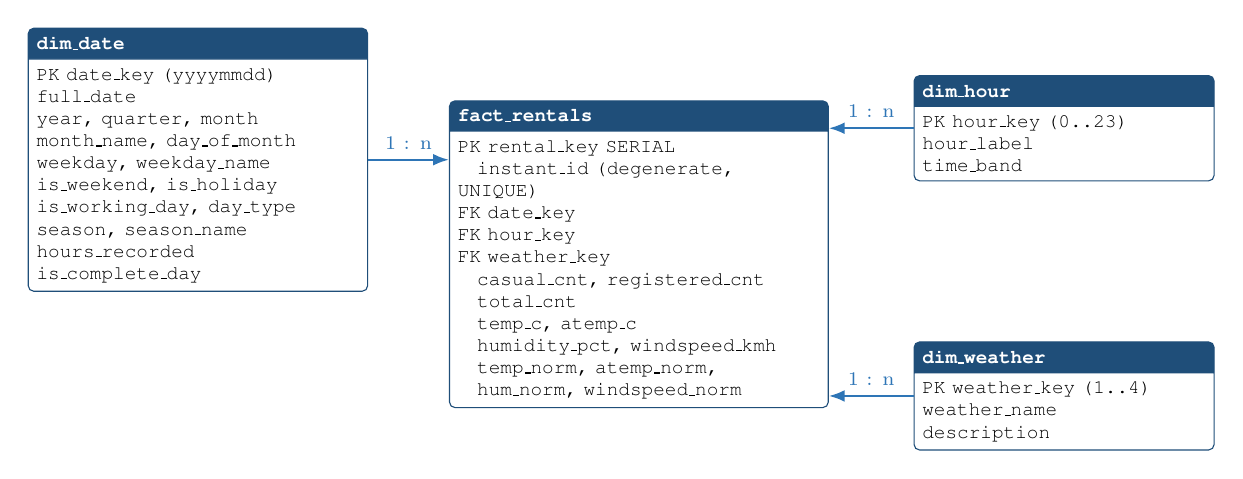
\begin{tikzpicture}[
  tbl/.style={draw=heading1, rectangle split, rectangle split parts=2, rectangle split part fill={heading1,white},
              rounded corners=2pt, font=\scriptsize\ttfamily, align=left, inner sep=3pt, text width=#1},
  tbl/.default=4.1cm, rel/.style={-{Latex[length=2mm]}, thick, heading2}]
\node[tbl=4.6cm] (fact) at (0,0) {\textcolor{white}{\textbf{fact\_rentals}} \nodepart{two}
  PK rental\_key SERIAL\\ \ \ \ instant\_id (degenerate, UNIQUE)\\ FK date\_key\\ FK hour\_key\\ FK weather\_key\\
  \ \ \ casual\_cnt, registered\_cnt\\ \ \ \ total\_cnt\\ \ \ \ temp\_c, atemp\_c\\ \ \ \ humidity\_pct, windspeed\_kmh\\
  \ \ \ temp\_norm, atemp\_norm,\\ \ \ \ hum\_norm, windspeed\_norm};
\node[tbl] (date) at (-5.6,1.2) {\textcolor{white}{\textbf{dim\_date}} \nodepart{two}
  PK date\_key (yyyymmdd)\\ full\_date\\ year, quarter, month\\ month\_name, day\_of\_month\\ weekday, weekday\_name\\
  is\_weekend, is\_holiday\\ is\_working\_day, day\_type\\ season, season\_name\\ hours\_recorded\\ is\_complete\_day};
\node[tbl=3.6cm] (hour) at (5.4,1.6) {\textcolor{white}{\textbf{dim\_hour}} \nodepart{two}
  PK hour\_key (0..23)\\ hour\_label\\ time\_band};
\node[tbl=3.6cm] (weather) at (5.4,-1.8) {\textcolor{white}{\textbf{dim\_weather}} \nodepart{two}
  PK weather\_key (1..4)\\ weather\_name\\ description};
\draw[rel] (date.east) -- node[above, font=\scriptsize] {1 : n} (fact.west |- date.east);
\draw[rel] (hour.west) -- node[above, font=\scriptsize] {1 : n} (fact.east |- hour.west);
\draw[rel] (weather.west) -- node[above, font=\scriptsize] {1 : n} (fact.east |- weather.west);
\end{tikzpicture}
\caption{Lược đồ Star Schema của kho dữ liệu}
\label{fig:star}
\end{figure}

\sect{Mô tả các bảng}
\begin{table}[H]
\centering
\caption{Các bảng trong kho dữ liệu}
\label{tab:dw-tables}
\begin{tabularx}{\textwidth}{|l|r|X|}
\hline
\textbf{Bảng} & \textbf{Số dòng} & \textbf{Nội dung và phân cấp} \\ \hline
\code{fact\_rentals} & 17.379 & Sự kiện thuê xe theo giờ; ràng buộc \code{CHECK (total\_cnt = casual\_cnt + registered\_cnt)}, các lượt thuê $\ge 0$, \code{UNIQUE (date\_key, hour\_key)}. \\ \hline
\code{dim\_date} & 731 & Lịch đầy đủ 2011--2012. Phân cấp \textit{năm $\rightarrow$ quý $\rightarrow$ tháng $\rightarrow$ ngày}; phân cấp phụ \textit{mùa}; thuộc tính phân loại ngày: \code{is\_weekend}, \code{is\_holiday}, \code{is\_working\_day}, \code{day\_type} $\in$ \{Working day, Weekend, Holiday\}; thuộc tính chất lượng: \code{hours\_recorded} (số giờ có bản ghi trong nguồn, 1--24) và \code{is\_complete\_day} (= đủ 24 giờ). \\ \hline
\code{dim\_hour} & 24 & Giờ trong ngày; phân cấp \textit{khung giờ $\rightarrow$ giờ}: Đêm (0--5h), Sáng (6--9h), Trưa (10--15h), Chiều (16--19h), Tối (20--23h). \\ \hline
\code{dim\_weather} & 4 & Bốn mức thời tiết của nguồn với tên ngắn và mô tả đầy đủ. \\ \hline
\code{v\_rentals\_flat} & (view) & View đã nối sẵn bảng sự kiện với ba bảng chiều; là điểm truy cập duy nhất của OLAP, API và DSS. \\ \hline
\end{tabularx}
\end{table}
Ba chỉ mục B-tree trên các khóa ngoại (\code{idx\_fact\_date}, \code{idx\_fact\_hour}, \code{idx\_fact\_weather}) hỗ trợ các phép lọc slice/dice và phép nối.

\sect{Các vấn đề thiết kế và quyết định của nhóm}\label{sec:design-issues}
\begin{table}[H]
\centering
\caption{Các vấn đề thiết kế kho dữ liệu và cách giải quyết}
\label{tab:design-issues}
\small
\begin{tabularx}{\textwidth}{|p{3.3cm}|X|}
\hline
\textbf{Vấn đề} & \textbf{Quyết định và lý do} \\ \hline
Chọn độ hạt & Theo giờ (mức nhỏ nhất của nguồn). Mức ngày sẽ làm mất thông tin giờ cao điểm - vốn là trọng tâm của DSS. \\ \hline
Star hay Snowflake & Chọn \textbf{Star}. Các chiều rất nhỏ (731, 24, 4 dòng), chuẩn hóa thêm (tách mùa, tháng, khung giờ thành bảng riêng) không tiết kiệm đáng kể mà làm truy vấn thêm phép nối. \\ \hline
Khóa của chiều & \code{date\_key} dạng số \code{yyyymmdd} (khóa thay thế ``thông minh'' dễ đọc, sắp xếp đúng thứ tự thời gian); \code{hour\_key}, \code{weather\_key} giữ mã tự nhiên vì ổn định. \\ \hline
Chiều suy biến & \code{instant\_id} (khóa dòng nguồn) lưu trong bảng sự kiện với ràng buộc \code{UNIQUE} để truy vết về nguồn và chống nạp trùng. \\ \hline
Chiều thay đổi chậm (SCD) & Các chiều mang tính tĩnh (lịch, giờ, mức thời tiết) nên không cần SCD; nếu sau này bổ sung chiều Trạm (địa chỉ, sức chứa thay đổi) sẽ dùng SCD loại 2. \\ \hline
Mùa và loại ngày & Đặt trong \code{dim\_date} (thuộc tính của ngày) thay vì tách chiều riêng. \code{day\_type} ưu tiên \textit{Holiday} $>$ \textit{Weekend} $>$ \textit{Working day} để mỗi ngày thuộc đúng một loại. \\ \hline
Thuộc tính thời tiết chuẩn hóa & Lưu \textbf{cả hai} dạng: giá trị gốc (\code{*\_norm}) để truy vết, giá trị quy đổi ($^\circ$C, \%, km/h theo Readme UCI) để trực quan hóa. Được xem là độ đo không cộng được, chỉ dùng \code{AVG}. \\ \hline
Giờ bị thiếu (165 giờ) & \textbf{Không tự sinh dòng} giá trị 0: không có bản ghi không đồng nghĩa với không có nhu cầu (nhiều giờ trùng bão). Các chỉ số trung bình theo giờ chỉ tính trên giờ có bản ghi. Thay vào đó, \code{dim\_date} lưu \code{hours\_recorded} và cờ \code{is\_complete\_day} (76 ngày thiếu giờ) để phân tích theo ngày có thể lọc ngày không đầy đủ. \\ \hline
Dữ liệu bất thường & Không xóa dòng nào (lượt thuê vẫn đúng). 22 giờ có độ ẩm 0\% (ngày 10/03/2011, lỗi cảm biến) được nạp với \code{humidity\_pct = NULL}, giữ giá trị gốc \code{hum\_norm} để truy vết; các phân tích độ ẩm tự loại các dòng này. 2.180 giờ (12,5\%) có tốc độ gió 0 được giữ nguyên nhưng ghi chú cần thận trọng. Các nhóm ít mẫu ($<30$ giờ) như mức thời tiết 4 được gắn cờ. \\ \hline
Chiến lược nạp & Nạp toàn bộ, \textbf{idempotent}: mỗi lần chạy xóa và tạo lại schema \code{dw} trong một giao dịch - phù hợp dữ liệu tĩnh; hướng nạp tăng dần được nêu ở mục~\ref{sec:limits}. \\ \hline
Toàn vẹn dữ liệu & Khóa chính, khóa ngoại, \code{CHECK} miền giá trị ở cả ba chiều và bảng sự kiện, \code{UNIQUE} trên khóa nghiệp vụ. \\ \hline
\end{tabularx}
\end{table}

\sect{Đoạn mã định nghĩa bảng sự kiện}
\begin{lstlisting}[language=SQL, caption={Định nghĩa bảng sự kiện (trích \code{sql/01\_schema.sql})}]
CREATE TABLE fact_rentals (
    rental_key      SERIAL PRIMARY KEY,
    instant_id      INTEGER NOT NULL UNIQUE,      -- degenerate dimension
    date_key        INTEGER  NOT NULL REFERENCES dim_date(date_key),
    hour_key        SMALLINT NOT NULL REFERENCES dim_hour(hour_key),
    weather_key     SMALLINT NOT NULL REFERENCES dim_weather(weather_key),
    casual_cnt      INTEGER NOT NULL CHECK (casual_cnt >= 0),
    registered_cnt  INTEGER NOT NULL CHECK (registered_cnt >= 0),
    total_cnt       INTEGER NOT NULL CHECK (total_cnt >= 0),
    temp_norm NUMERIC(6,4) NOT NULL, ...,  temp_c NUMERIC(5,2) NOT NULL, ...,
    humidity_pct    NUMERIC(5,2),         -- hum * 100; NULL khi hum = 0 (loi cam bien)
    CONSTRAINT chk_total CHECK (total_cnt = casual_cnt + registered_cnt),
    UNIQUE (date_key, hour_key)
);
CREATE INDEX idx_fact_date    ON fact_rentals(date_key);
CREATE INDEX idx_fact_hour    ON fact_rentals(hour_key);
CREATE INDEX idx_fact_weather ON fact_rentals(weather_key);
\end{lstlisting}

% ==================== CHƯƠNG 6 ====================
\newpage
\chap{Quy trình ETL}\label{sec:etl}

\sect{Tổng quan quy trình}
Quy trình ETL được hiện thực bằng Python (Pandas, psycopg2) trong thư mục \code{src/etl/}, chạy bằng một lệnh duy nhất \code{python src/etl/run\_etl.py}. Hình~\ref{fig:etl} mô tả luồng xử lý.

\begin{figure}[H]
\centering
\begin{tikzpicture}[node distance=0.45cm,
  box/.style={draw=heading1, fill=heading1!8, rounded corners=3pt, align=center, font=\footnotesize, minimum height=1.25cm, text width=2.15cm},
  src/.style={box, fill=gray!12, draw=gray},
  arr/.style={-{Latex[length=2mm]}, thick, heading2}]
\node[src] (csv) {\textbf{Nguồn}\\ hour.csv\\ day.csv};
\node[box, right=of csv] (ext) {\textbf{Extract}\\ extract.py\\ đọc CSV};
\node[box, right=of ext] (tr) {\textbf{Transform}\\ transform.py\\ làm sạch, tạo chiều};
\node[box, right=of tr] (ld) {\textbf{Load}\\ load.py\\ COPY, 1 giao dịch};
\node[box, right=of ld, fill=primary!12, draw=primary] (val) {\textbf{Validate}\\ validate.py\\ 13 phép đối chiếu};
\draw[arr] (csv) -- (ext); \draw[arr] (ext) -- (tr); \draw[arr] (tr) -- (ld); \draw[arr] (ld) -- (val);
\node[src, below=0.9cm of ld, text width=3.2cm] (dw) {\textbf{PostgreSQL}\\ schema \code{dw} + view};
\node[src, below=0.9cm of val, text width=2.6cm] (rep) {docs/\\validation\_report.md};
\draw[arr] (ld) -- (dw); \draw[arr] (val) -- (rep);
\end{tikzpicture}
\caption{Luồng xử lý ETL (\code{hour.csv} được nạp; \code{day.csv} chỉ dùng ở bước đối chiếu)}
\label{fig:etl}
\end{figure}

\sect{Extract}
Đọc \code{hour.csv} và \code{day.csv} bằng Pandas từ thư mục cấu hình \code{DATA\_DIR}. Cấu hình kết nối CSDL lấy từ tệp \code{.env} (không đưa mật khẩu vào mã nguồn).

\sect{Transform}
Hàm \code{clean()} thực hiện các bước tiền xử lý (FR02):
\begin{enumerate}
    \item Kiểm tra đủ 17 cột bắt buộc; thiếu cột thì dừng ETL.
    \item Chuyển \code{dteday} sang kiểu ngày theo định dạng \code{\%Y-\%m-\%d}.
    \item Đếm giá trị \code{null}, dòng trùng, \code{instant} trùng; nếu có thì ghi cảnh báo vào log và loại bỏ.
    \item Loại các dòng vi phạm \code{cnt = casual + registered} (có ghi log).
    \item Kiểm tra miền giá trị: \code{season} $\in [1,4]$, \code{hr} $\in [0,23]$, \code{weekday} $\in [0,6]$, \code{weathersit} $\in [1,4]$, các cờ $\in \{0,1\}$, \code{mnth} $\in [1,12]$, các thuộc tính chuẩn hóa $\in [0,1]$; vi phạm thì dừng ETL.
    \item Kiểm tra tính nhất quán của lịch: \code{yr}, \code{mnth}, \code{weekday} phải khớp với \code{dteday}; \code{season}, \code{holiday}, \code{workingday} phải giống nhau ở mọi giờ trong cùng một ngày (vì \code{dim\_date} chỉ lấy một giá trị mỗi ngày); vi phạm thì dừng ETL.
    \item Phát hiện giá trị bất thường nhưng \textbf{giữ dòng} (lượt thuê vẫn đúng) và ghi log: 22 dòng \code{hum = 0} (lỗi cảm biến, xử lý ở \code{build\_fact()}) và 2.180 dòng \code{windspeed = 0} (có thể là thiếu dữ liệu, giữ nguyên).
\end{enumerate}
Sau đó các bảng được dựng:
\begin{itemize}
    \item \code{build\_dim\_date()}: sinh \textbf{lịch liên tục} từ ngày nhỏ nhất đến lớn nhất, ghép thuộc tính mùa, ngày lễ, ngày làm việc từ nguồn; nếu có ngày trong lịch mà nguồn không có thì dừng (đảm bảo 731 ngày). Tạo khóa \code{yyyymmdd}, quý, tên tháng, tên thứ, \code{is\_weekend}, \code{day\_type}; đếm số giờ có bản ghi mỗi ngày (\code{hours\_recorded}) và cờ \code{is\_complete\_day}.
    \item \code{build\_dim\_hour()}: 24 giờ, nhãn \code{08:00-08:59}, khung giờ (\code{time\_band}).
    \item \code{build\_dim\_weather()}: 4 mức thời tiết với tên và mô tả theo Readme UCI.
    \item \code{build\_fact()}: ánh xạ khóa ngoại, giữ độ đo chuẩn hóa và quy đổi: $temp \times 41$, $atemp \times 50$, $hum \times 100$, $windspeed \times 67$; riêng \code{humidity\_pct} được đặt \code{NULL} khi \code{hum = 0} (vẫn giữ \code{hum\_norm} gốc).
\end{itemize}

\sect{Load}
Hàm \code{create\_schema()} chạy \code{sql/01\_schema.sql} (xóa và tạo lại schema \code{dw}). Các bảng được nạp theo thứ tự \code{dim\_date} $\rightarrow$ \code{dim\_hour} $\rightarrow$ \code{dim\_weather} $\rightarrow$ \code{fact\_rentals} bằng lệnh \code{COPY ... FROM STDIN} (nạp theo lô, nhanh hơn nhiều so với \code{INSERT} từng dòng), \textbf{trong một giao dịch}: lỗi ở bất kỳ bảng nào thì \code{ROLLBACK}, không để kho ở trạng thái nạp dở. Cuối cùng chạy \code{ANALYZE} để cập nhật thống kê cho bộ tối ưu truy vấn và tạo view \code{v\_rentals\_flat} (\code{sql/02\_views.sql}).

\sect{Đối chiếu sau khi nạp (Validate)}
Hàm \code{validate()} so sánh kho với cả hai tệp nguồn và ghi kết quả ra \code{docs/validation\_report.md}. ETL trả về mã lỗi khác 0 nếu có phép đối chiếu thất bại. Kết quả lần chạy cuối:

\begin{table}[H]
\centering
\caption{Kết quả đối chiếu ETL}
\label{tab:etl-validate}
\begin{tabularx}{\textwidth}{|X|r|r|c|}
\hline
\textbf{Kiểm tra} & \textbf{Kỳ vọng} & \textbf{Thực tế} & \textbf{Kết quả} \\ \hline
Số dòng fact = số dòng \code{hour.csv} & 17.379 & 17.379 & PASS \\ \hline
Tổng \code{cnt} (fact và \code{hour.csv}) & 3.292.679 & 3.292.679 & PASS \\ \hline
Tổng \code{casual} (fact và \code{hour.csv}) & 620.017 & 620.017 & PASS \\ \hline
Tổng \code{registered} (fact và \code{hour.csv}) & 2.672.662 & 2.672.662 & PASS \\ \hline
Tổng \code{cnt} (fact và \code{day.csv}) & 3.292.679 & 3.292.679 & PASS \\ \hline
Số ngày \code{dim\_date} = số dòng \code{day.csv} & 731 & 731 & PASS \\ \hline
Số dòng \code{dim\_hour} & 24 & 24 & PASS \\ \hline
Số dòng fact mồ côi (vi phạm khóa ngoại) & 0 & 0 & PASS \\ \hline
Số dòng vi phạm \code{cnt = casual + registered} & 0 & 0 & PASS \\ \hline
Số ngày có tổng \code{cnt} lệch \code{day.csv} & 0 & 0 & PASS \\ \hline
Tổng \code{hours\_recorded} (\code{dim\_date}) = số dòng \code{hour.csv} & 17.379 & 17.379 & PASS \\ \hline
Số ngày thiếu giờ (\code{is\_complete\_day = false}) & 76 & 76 & PASS \\ \hline
Số dòng \code{humidity\_pct} NULL = số dòng \code{hum = 0} ở nguồn & 22 & 22 & PASS \\ \hline
\end{tabularx}
\end{table}
Phép đối chiếu theo từng ngày với \code{day.csv} là bằng chứng mạnh nhất cho tính chính xác (NFR01): tổng theo giờ của cả 731 ngày đều khớp với tệp tổng hợp theo ngày, độc lập với tệp dùng để nạp.

% ==================== CHƯƠNG 7 ====================
\newpage
\chap{Hiện thực hệ thống}\label{sec:impl}

\sect{Kiến trúc tổng thể}\label{sec:arch}
Hệ thống theo kiến trúc nhiều tầng (Hình~\ref{fig:arch}): tầng nguồn dữ liệu, tầng ETL, tầng kho dữ liệu, tầng dịch vụ (OLAP API và mô hình DSS) và tầng trình bày (dashboard). Kho dữ liệu đóng vai trò \textbf{phân hệ quản lý dữ liệu} chung cho cả phân tích OLAP và DSS.

\begin{figure}[H]
\centering
\begin{tikzpicture}[node distance=0.5cm and 0.6cm,
  layer/.style={draw=gray!60, rounded corners=4pt, fill=gray!5, inner sep=6pt},
  box/.style={draw=heading1, fill=white, rounded corners=3pt, align=center, font=\footnotesize, text width=2.7cm, minimum height=1.0cm},
  arr/.style={-{Latex[length=2mm]}, thick, heading2}]
\node[box, fill=gray!12] (csv) {\textbf{CSV nguồn}\\ hour.csv, day.csv};
\node[box, right=of csv] (etl) {\textbf{ETL (Python)}\\ extract, transform,\\ load, validate};
\node[box, right=of etl, fill=heading1!10, text width=3.2cm] (dw) {\textbf{PostgreSQL}\\ schema \code{dw}: Star Schema\\ view \code{v\_rentals\_flat}};
\node[box, below=1.1cm of dw, text width=3.2cm] (api) {\textbf{FastAPI}\\ OLAP, KPI, climate\\ \code{/api/dss/*}};
\node[box, left=of api, fill=primary!12, draw=primary] (dss) {\textbf{Mô hình DSS}\\ \code{src/dss/engine.py}\\ ngưỡng, phân loại,\\ khuyến nghị};
\node[box, below=1.1cm of api, text width=3.2cm] (ui) {\textbf{Dashboard React}\\ Vite, Recharts\\ bộ lọc, KPI, OLAP, DSS};
\node[box, left=of ui, fill=gray!12] (user) {\textbf{Người dùng}\\ quản lý vận hành,\\ nhà phân tích};
\draw[arr] (csv) -- (etl); \draw[arr] (etl) -- (dw);
\draw[arr] (dw) -- node[right, font=\scriptsize] {SQL chỉ đọc} (api);
\draw[arr, <->] (api) -- (dss);
\draw[arr] (api) -- node[right, font=\scriptsize] {JSON / HTTP} (ui);
\draw[arr, <->] (ui) -- (user);
\end{tikzpicture}
\caption{Kiến trúc tổng thể hệ thống}
\label{fig:arch}
\end{figure}

\sect{Công nghệ sử dụng}
\begin{table}[H]
\centering
\caption{Công nghệ sử dụng}
\begin{tabularx}{\textwidth}{|p{3.2cm}|p{4.2cm}|X|}
\hline
\textbf{Tầng} & \textbf{Công nghệ} & \textbf{Lý do lựa chọn} \\ \hline
Kho dữ liệu & PostgreSQL~\cite{postgres} & Hỗ trợ \code{GROUP BY ROLLUP}, \code{FILTER}, \code{percentile\_cont}, \code{corr} cho OLAP và DSS; mã nguồn mở \\ \hline
ETL & Python 3, Pandas, psycopg2 & Xử lý bảng linh hoạt; \code{COPY} nạp theo lô \\ \hline
API & FastAPI~\cite{fastapi}, Uvicorn & Kiểm tra tham số tự động, tài liệu OpenAPI tự sinh tại \code{/docs} \\ \hline
DSS & Python thuần (\code{src/dss}) & Tách khỏi CSDL để kiểm thử độc lập \\ \hline
Frontend & React 18~\cite{react}, Vite, Recharts~\cite{recharts} & Thành phần hóa giao diện, biểu đồ khai báo \\ \hline
Kiểm thử & pytest, FastAPI TestClient & Kiểm thử tự động API, OLAP, DSS \\ \hline
\end{tabularx}
\end{table}

\sect{Tổ chức mã nguồn}
\begin{lstlisting}[caption={Cấu trúc thư mục dự án}]
bike-dw/
|-- data/            hour.csv, day.csv, Readme_UCI.txt
|-- sql/             01_schema.sql   02_views.sql
|                    03_olap_queries.sql   04_dss_queries.sql
|-- src/
|   |-- etl/         config, extract, transform, load, validate, run_etl
|   |-- api/         main.py (endpoints), queries.py (OLAP/KPI),
|   |                dss_queries.py (truy xuat cho DSS), db.py
|   |-- dss/         engine.py (mo hinh DSS, khong phu thuoc CSDL)
|   `-- dashboard/   React: App.jsx, components/ (FilterBar, KpiCards,
|                    DrillChart, Charts, PivotTable, DssPanel)
|-- tests/           test_api, test_climate, test_dss_engine, test_dss_api
|-- docs/            validation_report.md
`-- report/          bao cao LaTeX
\end{lstlisting}
Mỗi tầng là một module riêng (NFR05): thay đổi giao diện không ảnh hưởng ETL; mô hình DSS không phụ thuộc CSDL.

\sect{Truy vấn OLAP}\label{sec:olap}
Tệp \code{sql/03\_olap\_queries.sql} chứa các truy vấn mẫu cho năm phép toán OLAP; API sinh truy vấn tương đương có tham số hóa.

\begin{lstlisting}[language=SQL, caption={Roll-up năm $\rightarrow$ tháng với tổng cấp trên}]
SELECT year, month, SUM(total_cnt) AS total_rentals
FROM v_rentals_flat
GROUP BY ROLLUP (year, month)        -- month IS NULL: subtotal of year
ORDER BY year, month;                -- last row: grand total
\end{lstlisting}

\begin{lstlisting}[language=SQL, caption={Drill-down: năm 2012 $\rightarrow$ quý 3 $\rightarrow$ tháng 7 $\rightarrow$ ngày $\rightarrow$ giờ}]
SELECT quarter, SUM(total_cnt) FROM v_rentals_flat WHERE year = 2012 GROUP BY quarter;
SELECT month_name, SUM(total_cnt) FROM v_rentals_flat
WHERE year = 2012 AND quarter = 3 GROUP BY month, month_name ORDER BY month;
SELECT full_date, SUM(total_cnt) FROM v_rentals_flat
WHERE year = 2012 AND month = 7 GROUP BY full_date ORDER BY full_date;
SELECT hour, total_cnt FROM v_rentals_flat WHERE full_date = '2012-07-06' ORDER BY hour;
\end{lstlisting}

\begin{lstlisting}[language=SQL, caption={Slice (một chiều) và Dice (nhiều chiều)}]
-- SLICE: weather = Clear
SELECT month_name, SUM(total_cnt) AS total, ROUND(AVG(total_cnt), 1) AS avg_hourly
FROM v_rentals_flat WHERE weather_name = 'Clear'
GROUP BY month, month_name ORDER BY month;
-- DICE: 2012, summer + fall, working day, morning + afternoon peak bands
SELECT hour, ROUND(AVG(total_cnt), 1) AS avg_hourly
FROM v_rentals_flat
WHERE year = 2012 AND season IN (2, 3) AND day_type = 'Working day'
  AND time_band IN (...)                  -- morning and afternoon bands
GROUP BY hour ORDER BY hour;
\end{lstlisting}

\begin{lstlisting}[language=SQL, caption={Pivot: hàng = tháng, cột = thời tiết}]
SELECT month_name,
  ROUND(AVG(total_cnt) FILTER (WHERE weather_key = 1), 1) AS clear,
  ROUND(AVG(total_cnt) FILTER (WHERE weather_key = 2), 1) AS mist,
  ROUND(AVG(total_cnt) FILTER (WHERE weather_key = 3), 1) AS light_rain_snow,
  ROUND(AVG(total_cnt) FILTER (WHERE weather_key = 4), 1) AS heavy_rain_snow
FROM v_rentals_flat GROUP BY month, month_name ORDER BY month;
\end{lstlisting}

\sect{Tầng dịch vụ (REST API)}
\begin{table}[H]
\centering
\caption{Các endpoint của API}
\label{tab:api}
\small
\begin{tabularx}{\textwidth}{|l|X|c|}
\hline
\textbf{Endpoint} & \textbf{Chức năng} & \textbf{Yêu cầu} \\ \hline
\code{/api/filters} & Danh sách giá trị cho bộ lọc & FR08 \\ \hline
\code{/api/kpis} & 8 KPI theo bộ lọc & FR08 \\ \hline
\code{/api/olap/drill} & Roll-up / drill-down năm $\rightarrow$ quý $\rightarrow$ tháng $\rightarrow$ ngày $\rightarrow$ giờ & FR05, FR07 \\ \hline
\code{/api/olap/pivot} & Bảng pivot 2 chiều tùy chọn (8 chiều), độ đo tổng hoặc trung bình & FR07 \\ \hline
\code{/api/hourly} & Hồ sơ nhu cầu theo giờ, tách ngày làm việc / ngày nghỉ & FR05, FR06 \\ \hline
\code{/api/weather}, \code{/api/day-type} & Nhu cầu theo thời tiết, theo loại ngày & FR06 \\ \hline
\code{/api/users} & Đăng ký và vãng lai theo giờ / thứ / tháng & FR06 \\ \hline
\code{/api/climate} & Nhu cầu theo khoảng nhiệt độ / độ ẩm, hệ số tương quan & FR06 \\ \hline
\code{/api/dss/thresholds} & Khảo sát phân phối, ngưỡng phân loại & FR09 \\ \hline
\code{/api/dss/plan} & Kế hoạch 24 giờ cho tình huống: phân loại, khuyến nghị, cảnh báo & FR09, FR10 \\ \hline
\code{/api/dss/matrix} & Ma trận phân loại giờ $\times$ loại ngày $\times$ thời tiết & FR09 \\ \hline
\end{tabularx}
\end{table}
Mọi endpoint phân tích dùng chung bộ lọc \code{year, season, month, weekday, weather, day\_type, time\_band} (nhiều giá trị cách nhau bởi dấu phẩy) - đây chính là phép \textbf{slice/dice} tổng quát. Về an toàn: tên cột và biểu thức đưa vào SQL chỉ lấy từ danh sách trắng (whitelist) trong mã; mọi giá trị từ người dùng đều được \textbf{tham số hóa}; kết nối CSDL ở chế độ chỉ đọc. Kiểm thử tự động xác nhận chuỗi tấn công SQL injection không có tác dụng (mục~\ref{sec:eval}).

\sect{Dashboard}
Dashboard (Hình~\ref{fig:dash-overview}--\ref{fig:dash-pivot}) gồm: thanh bộ lọc dạng chip đa chọn áp dụng cho mọi biểu đồ; 8 thẻ KPI; biểu đồ drill-down theo thời gian có breadcrumb (bấm vào cột để khoan xuống, bấm breadcrumb để cuộn lên); 4 biểu đồ phân tích (theo giờ, thời tiết, loại ngày, nhóm người dùng); biểu đồ nhiệt độ/độ ẩm kèm bảng tương quan; bảng pivot với hàng, cột, độ đo tùy chọn và tô màu theo giá trị; và khu vực DSS (mục~\ref{sec:dss-ui}).

\begin{figure}[H]
\centering
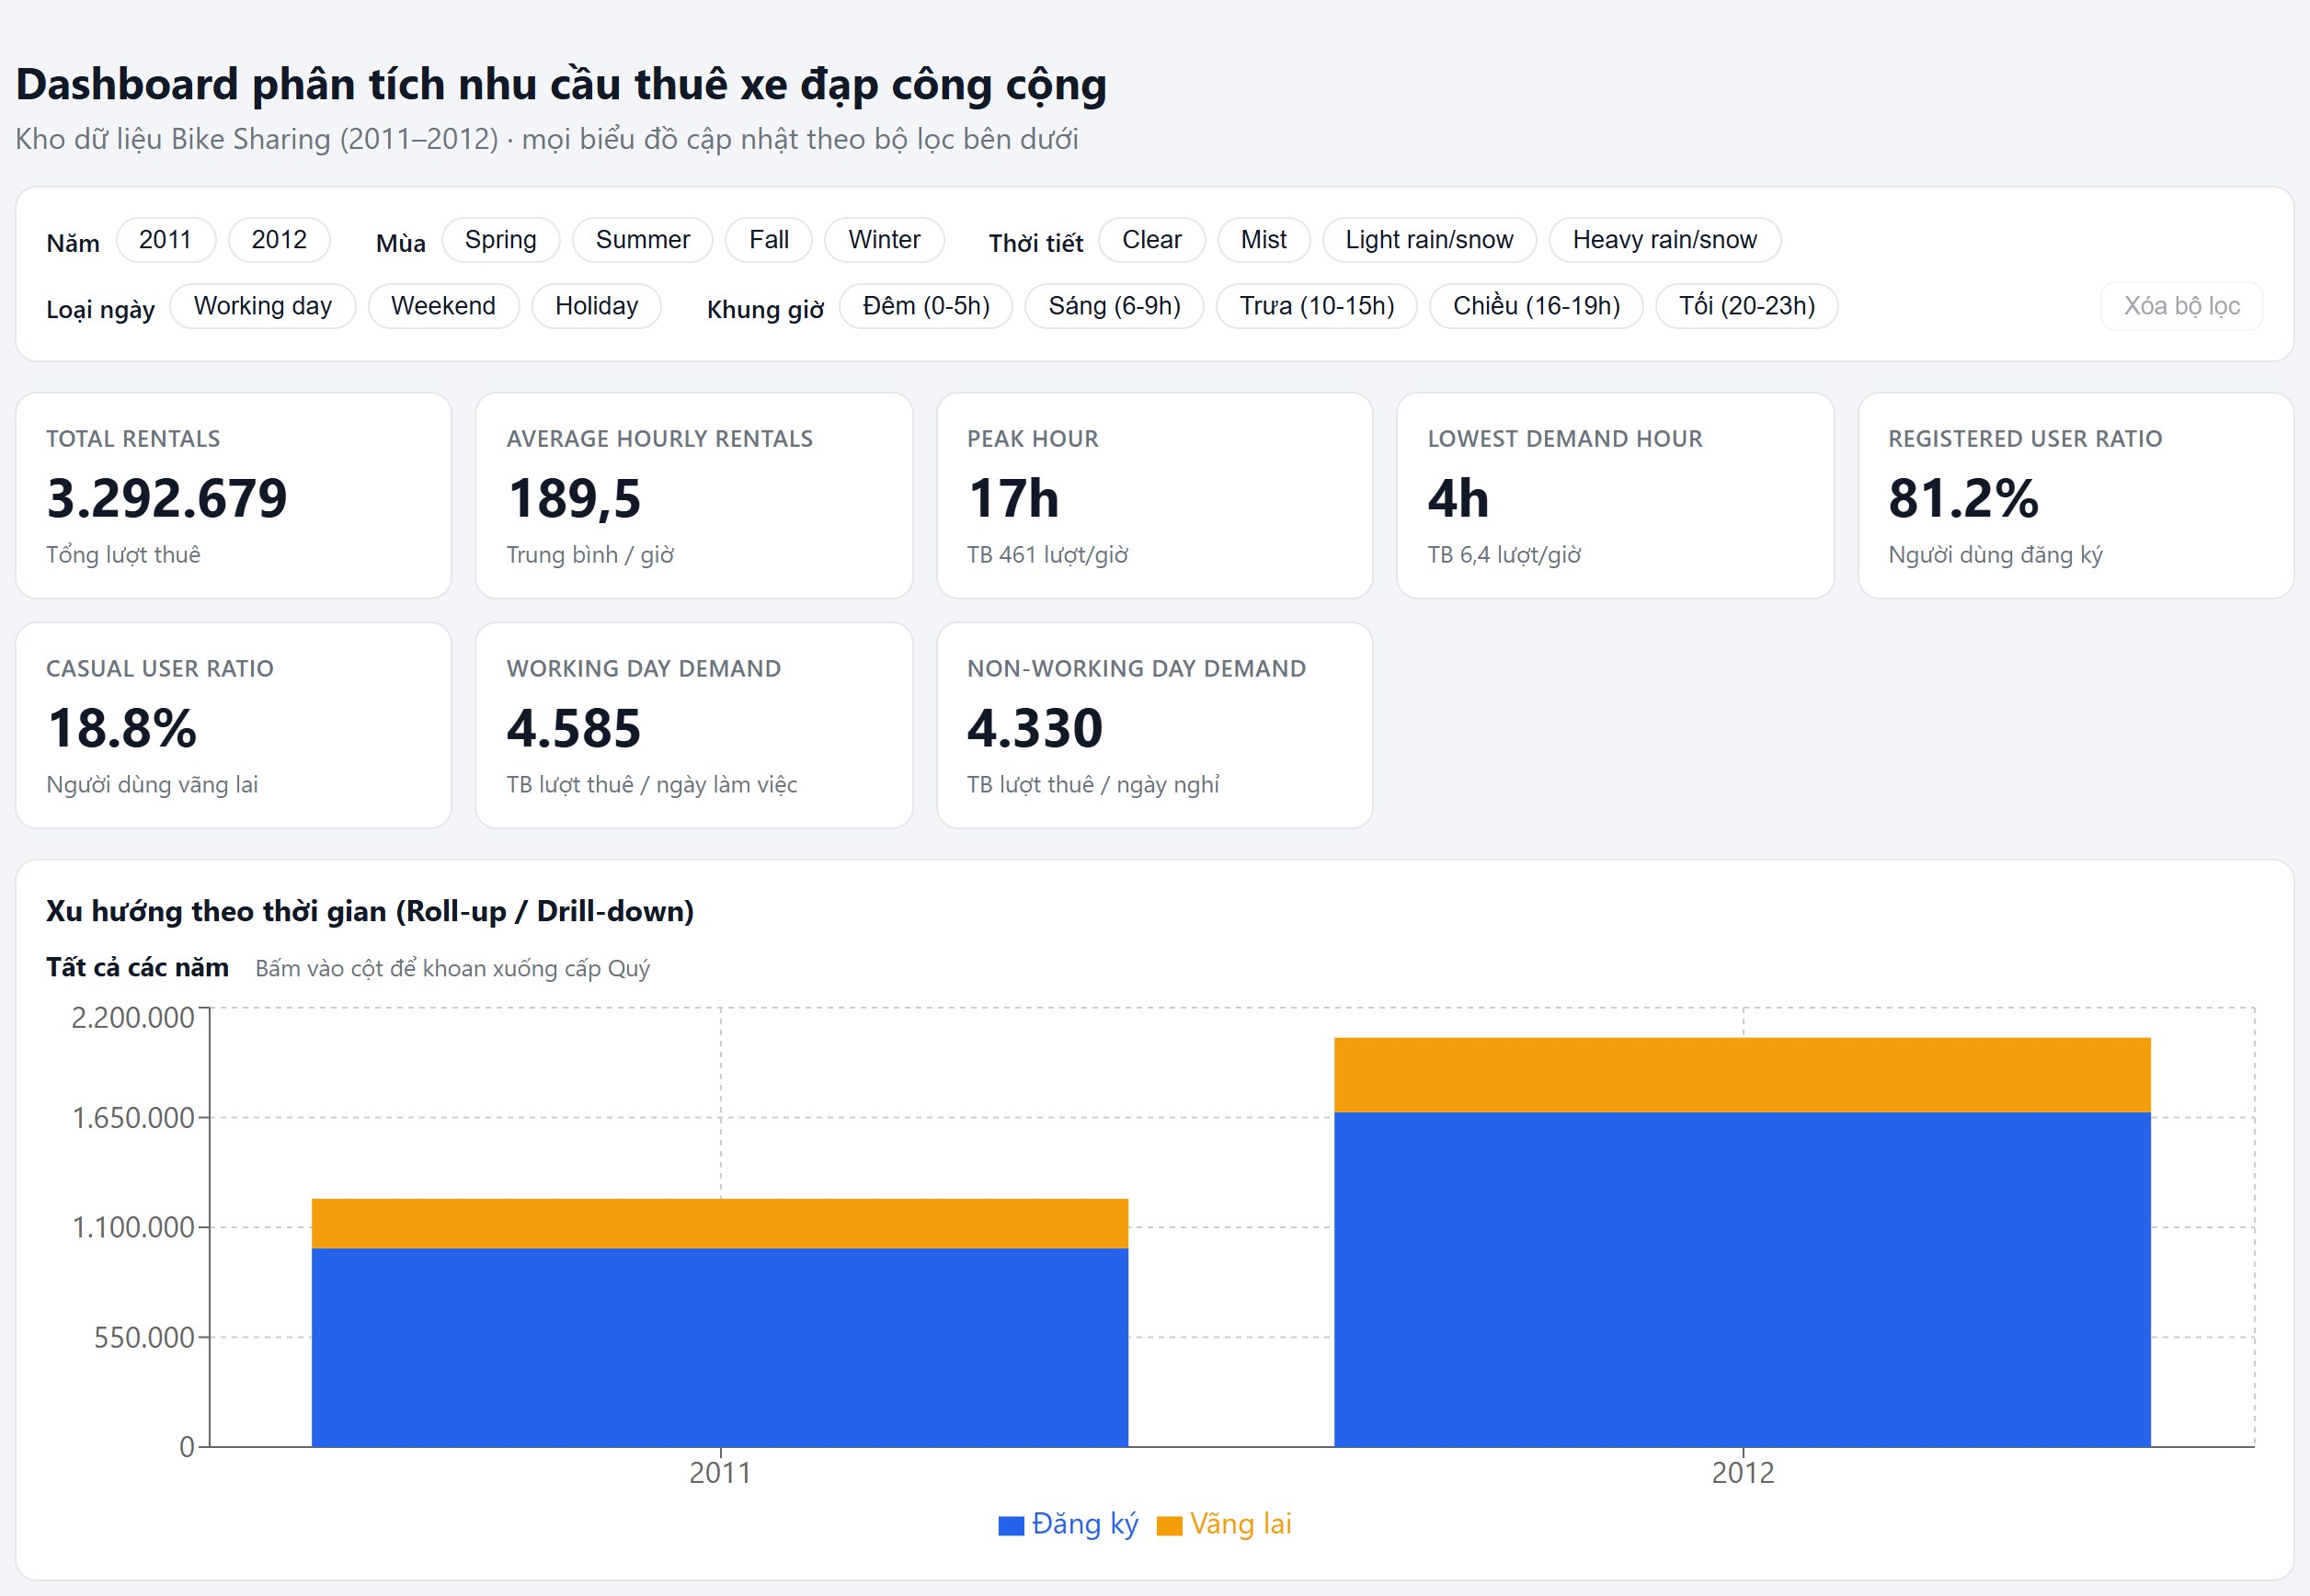
\includegraphics[width=\textwidth]{figures/dash_overview.jpg}
\caption{Dashboard: bộ lọc, 8 KPI và biểu đồ drill-down theo thời gian}
\label{fig:dash-overview}
\end{figure}

\begin{figure}[H]
\centering
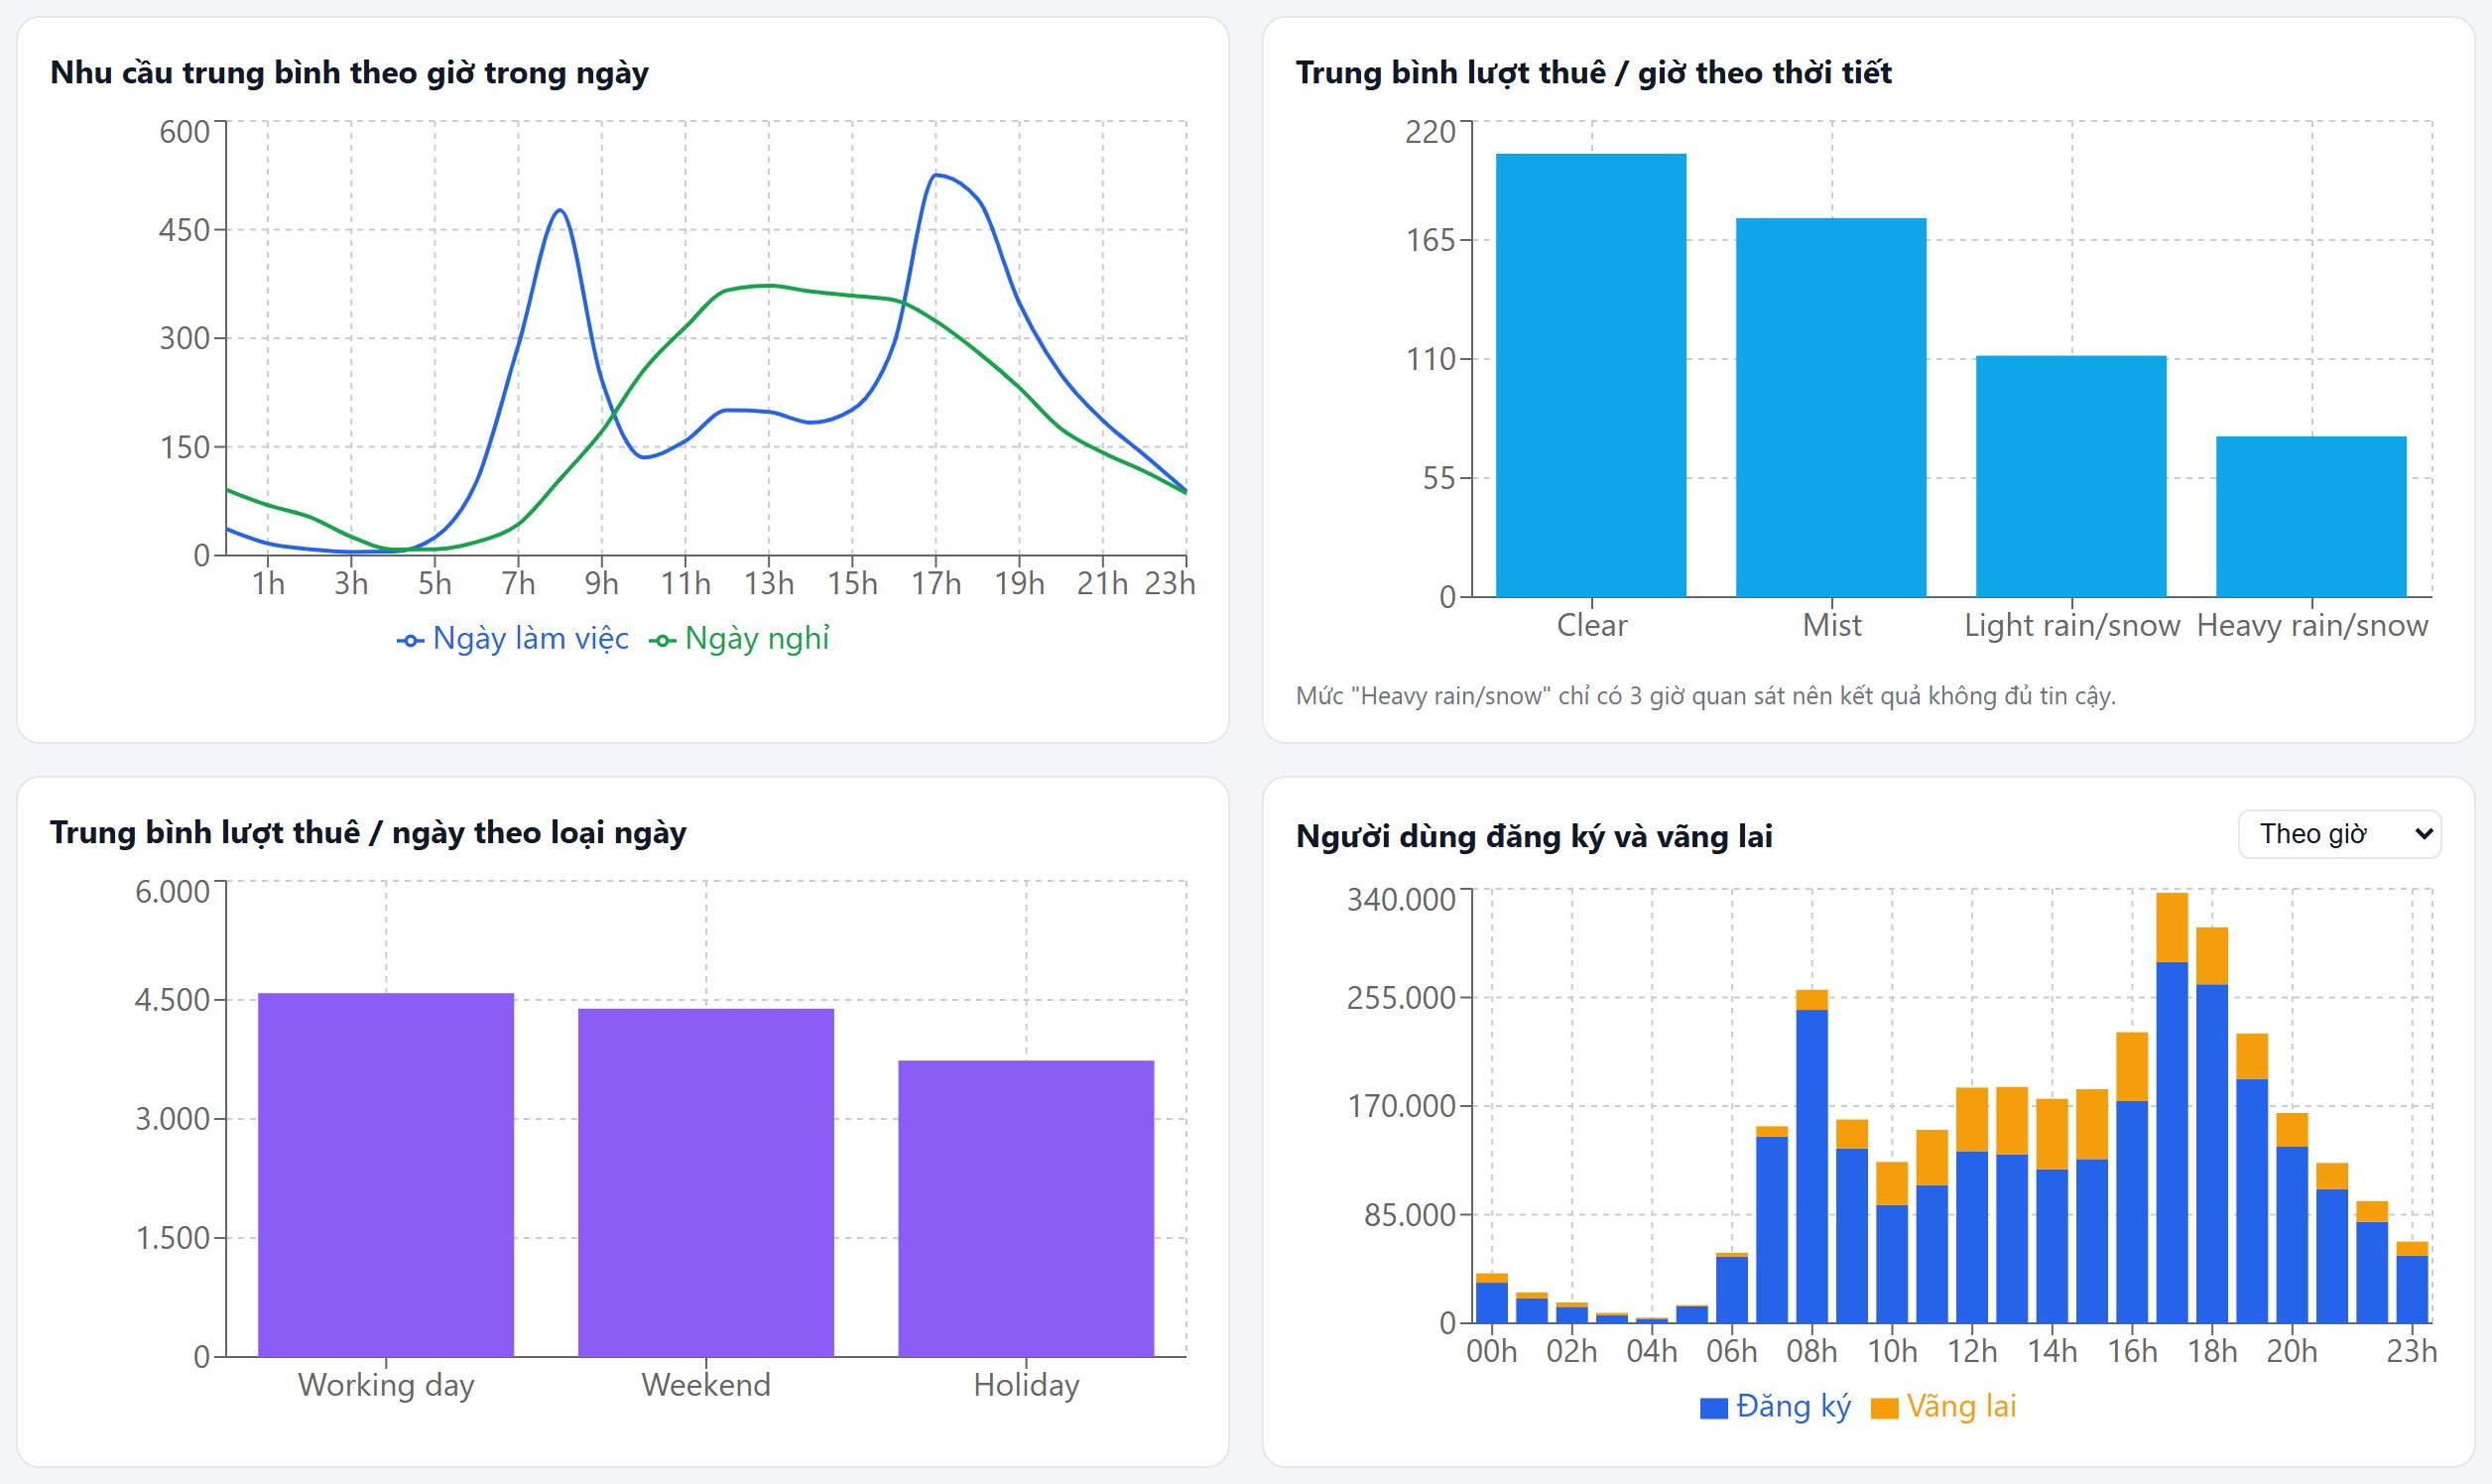
\includegraphics[width=\textwidth]{figures/dash_analysis.jpg}
\caption{Dashboard: phân tích theo giờ, thời tiết, loại ngày và nhóm người dùng}
\label{fig:dash-analysis}
\end{figure}

\begin{figure}[H]
\centering
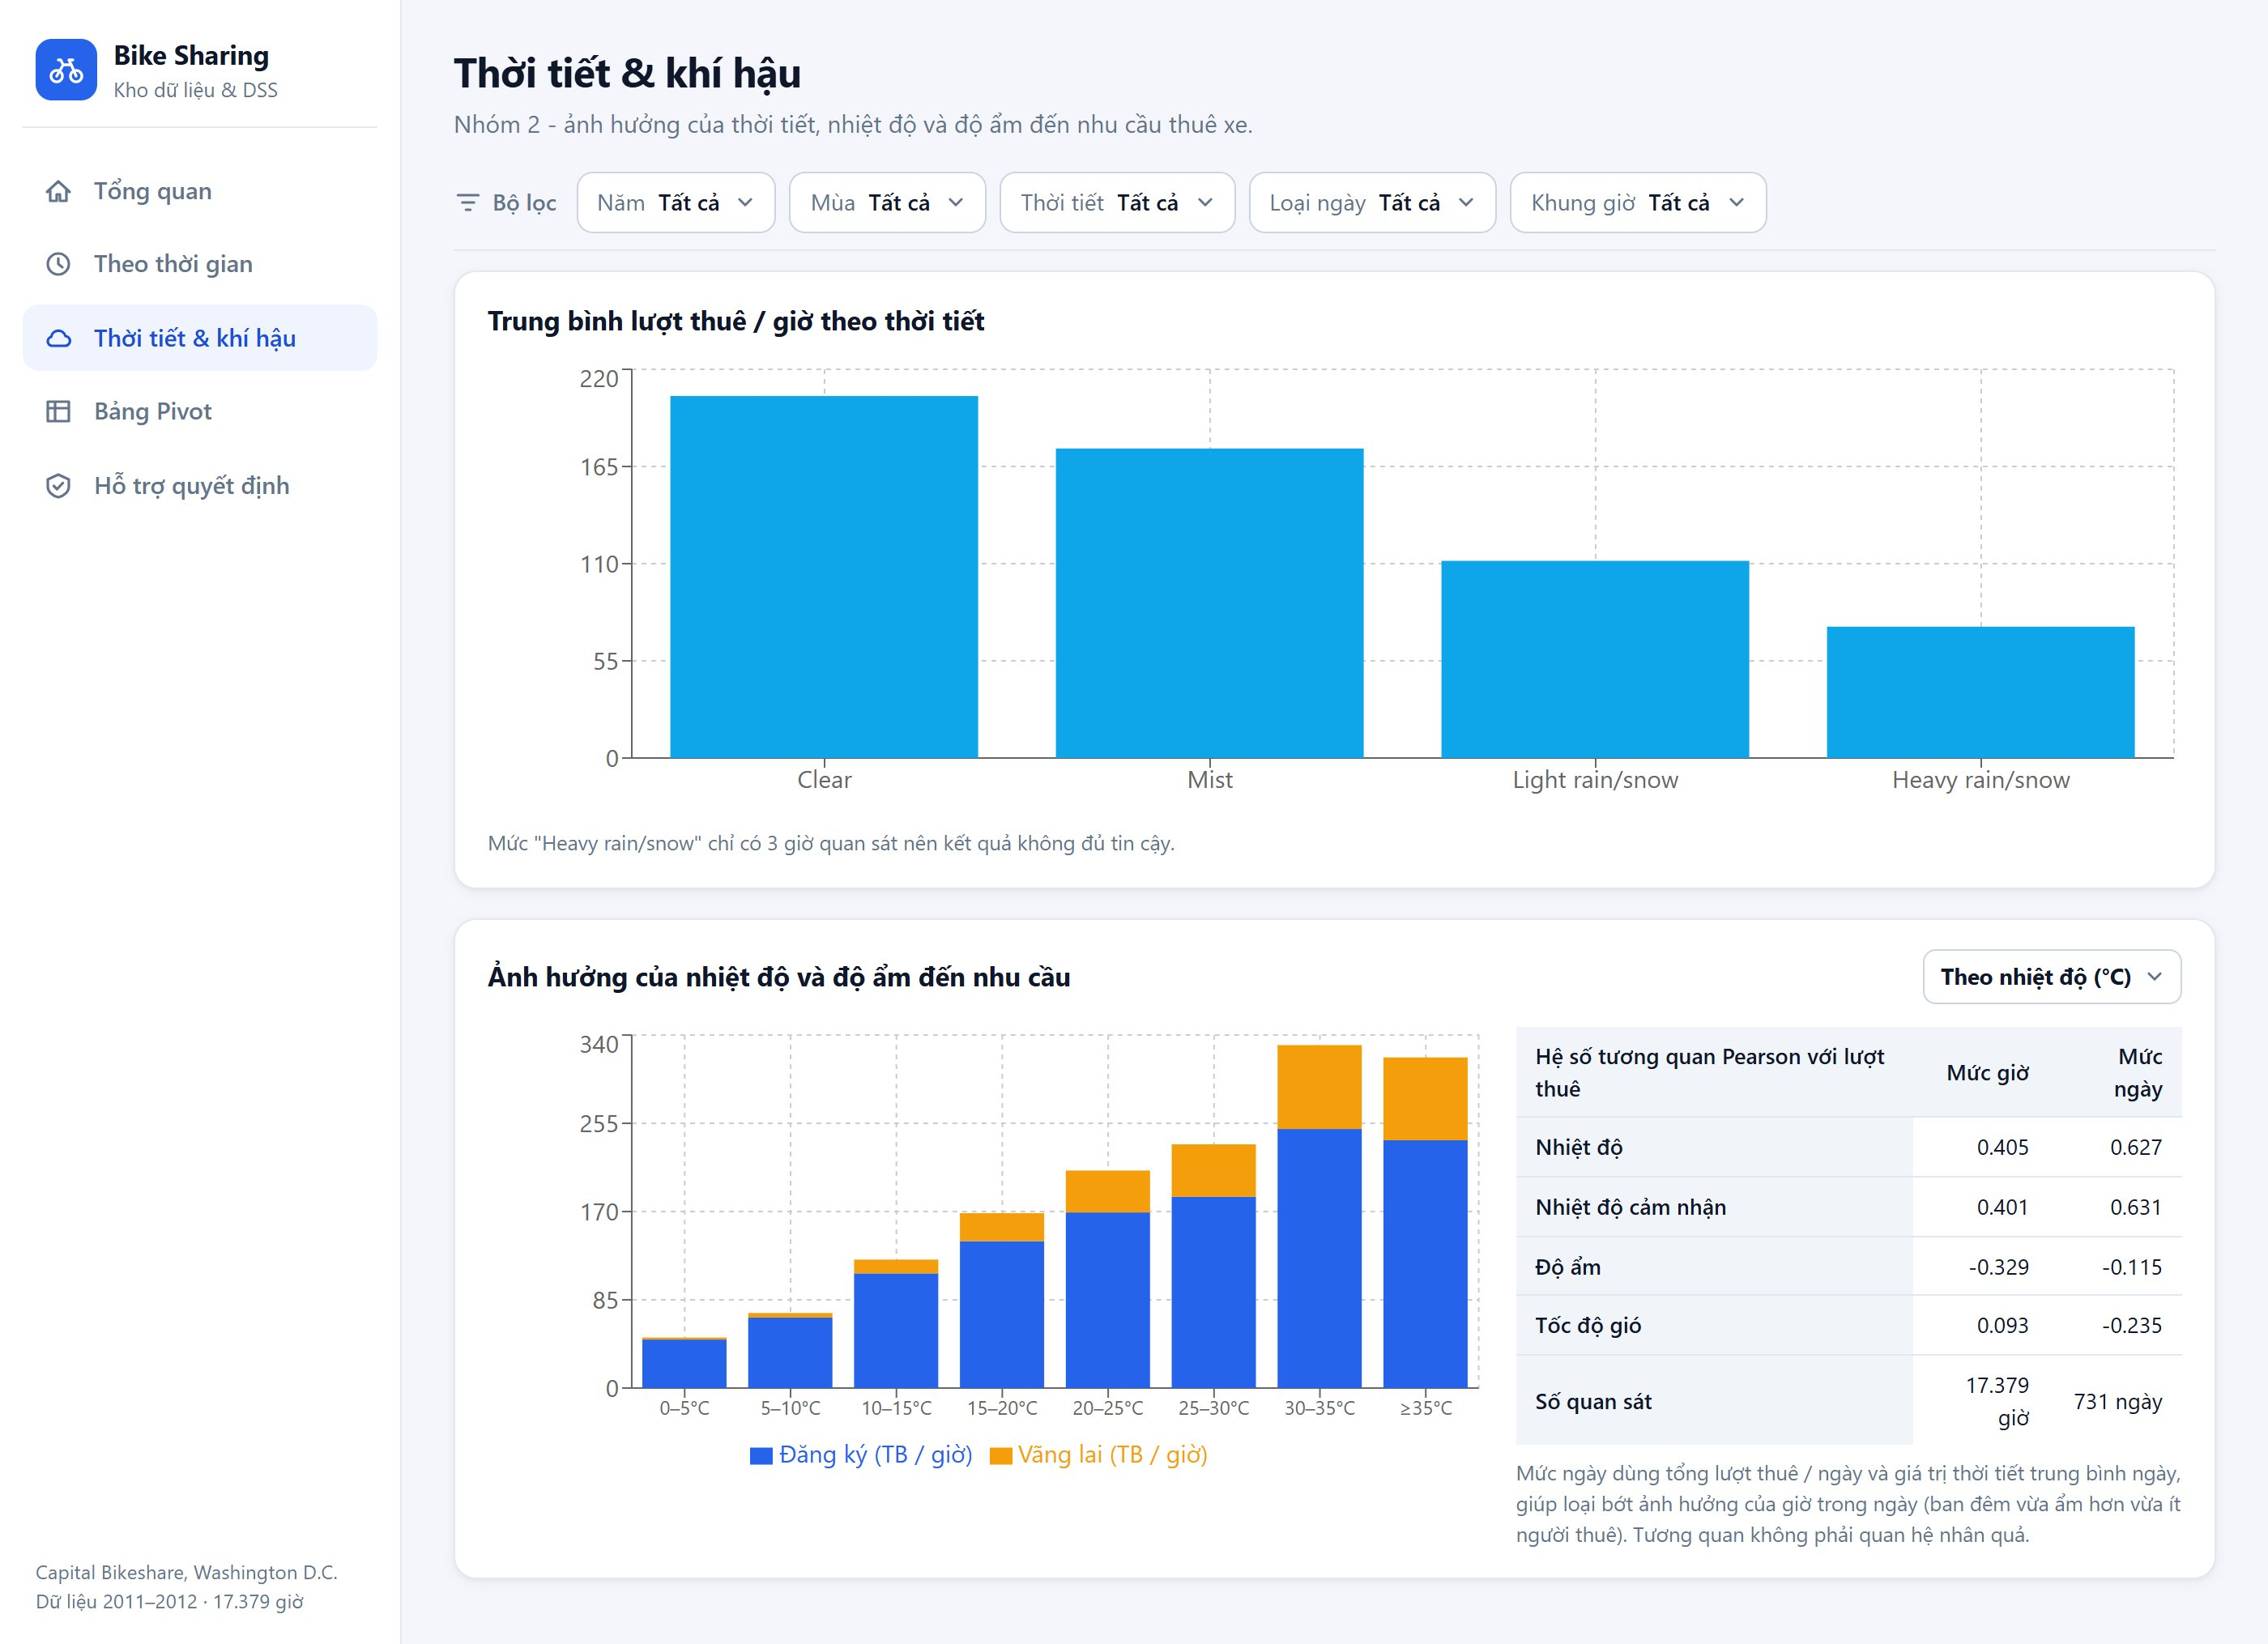
\includegraphics[width=\textwidth]{figures/dash_climate.jpg}
\caption{Dashboard: ảnh hưởng của nhiệt độ, độ ẩm và bảng hệ số tương quan}
\label{fig:dash-climate}
\end{figure}

\begin{figure}[H]
\centering
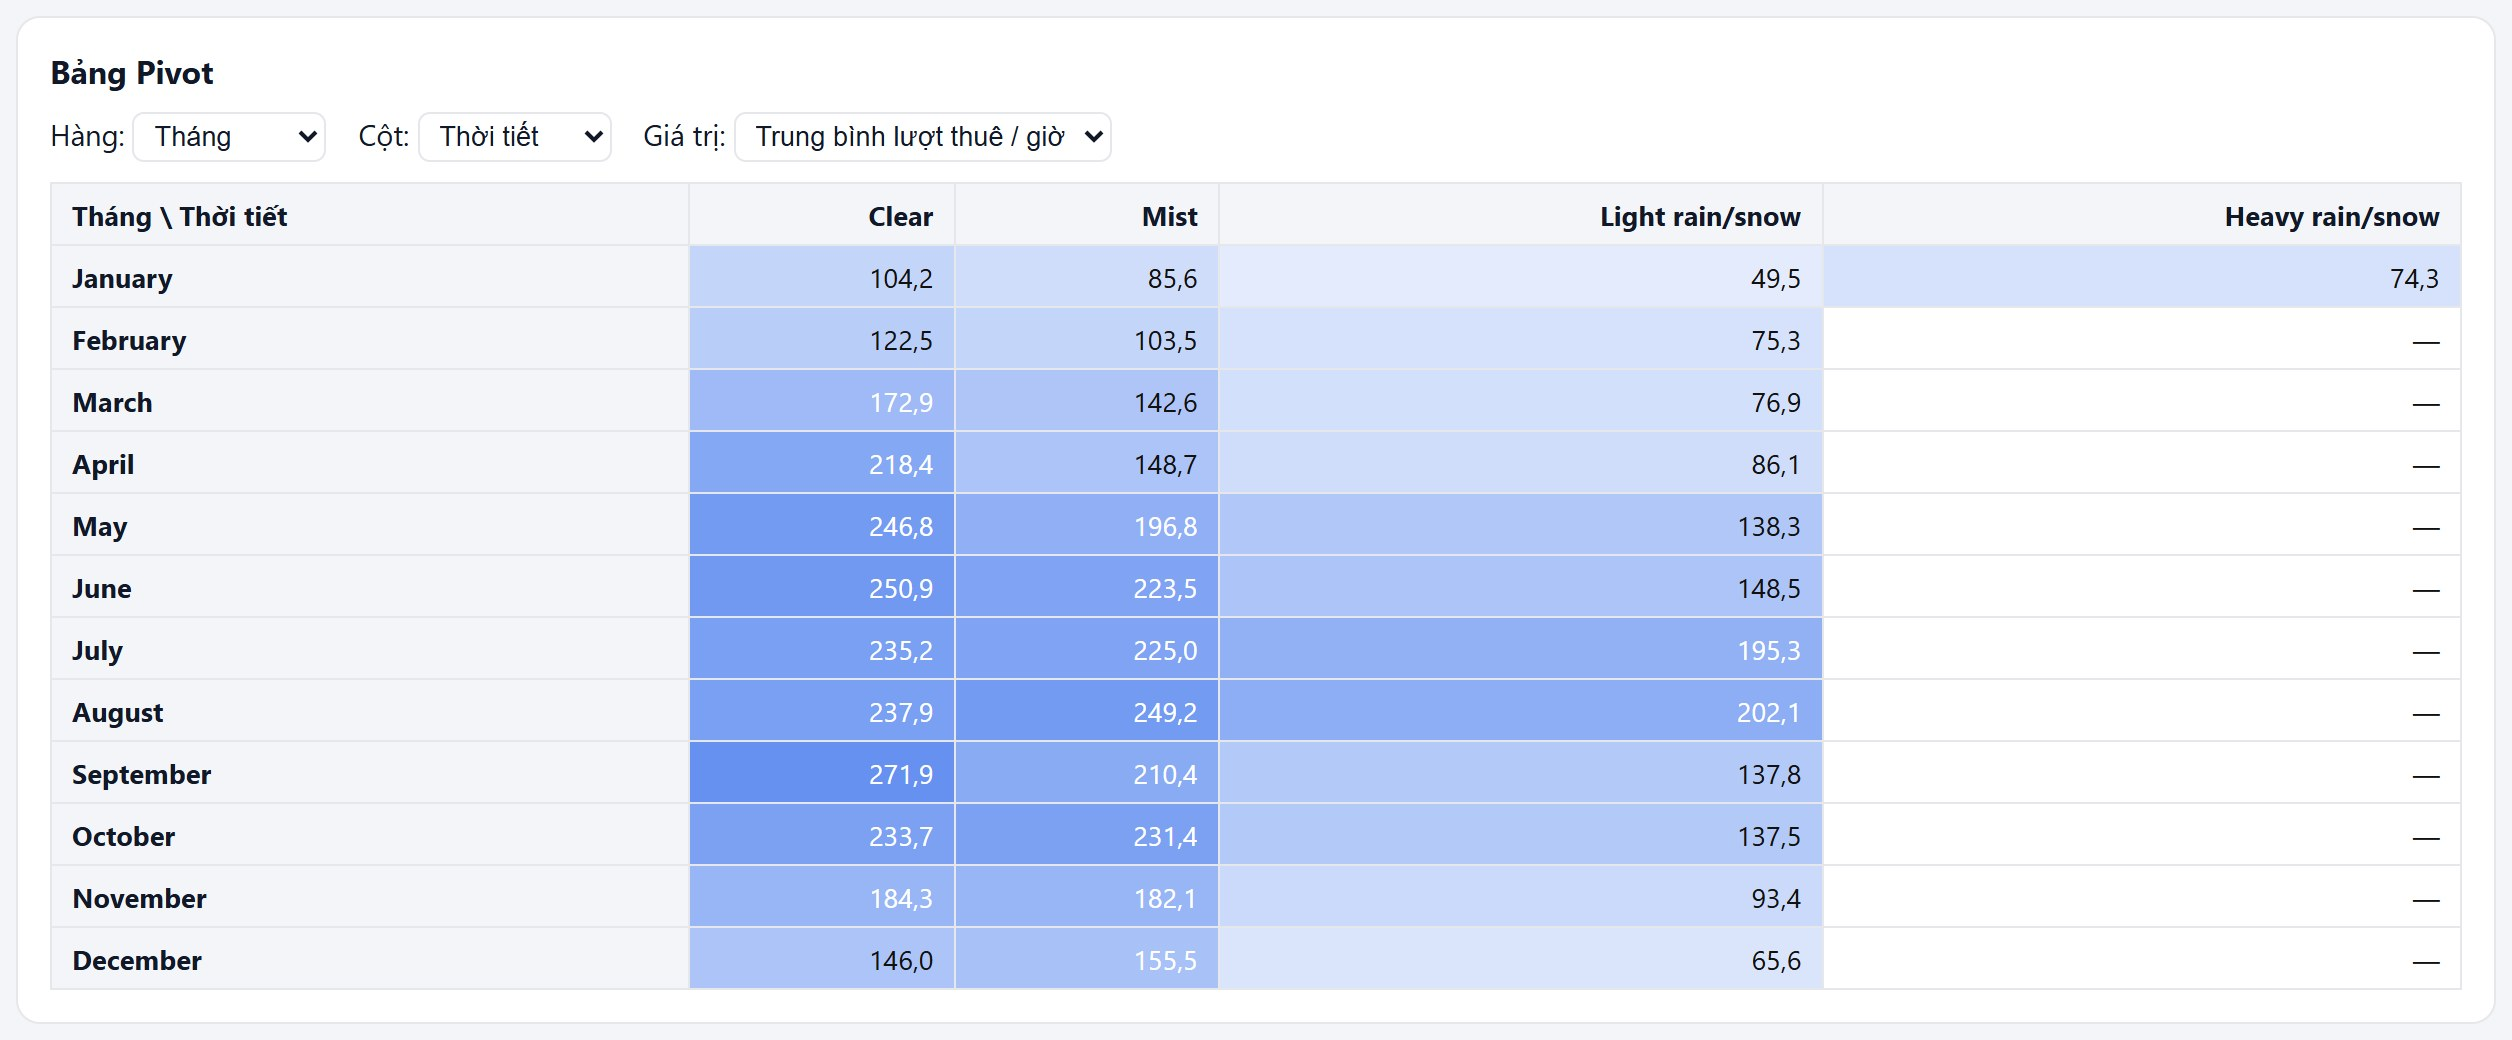
\includegraphics[width=\textwidth]{figures/dash_pivot.jpg}
\caption{Dashboard: bảng pivot tháng $\times$ thời tiết}
\label{fig:dash-pivot}
\end{figure}

% ==================== CHƯƠNG 8 ====================
\newpage
\chap{Thành phần hệ hỗ trợ quyết định (DSS)}\label{sec:dss}

\sect{Quyết định cần hỗ trợ}
Theo nguyên tắc thiết kế DSS (mục~\ref{sec:theory-dss}), nhóm xuất phát từ quyết định cần hỗ trợ:
\begin{itemize}
    \item \textbf{Người ra quyết định}: quản lý vận hành hệ thống xe đạp công cộng.
    \item \textbf{Quyết định}: với một ngày sắp tới (biết trước loại ngày và dự báo thời tiết), mỗi khung giờ cần chuẩn bị nguồn lực ở mức nào - cơ bản, theo dõi, hay tăng cường; khung giờ nào cần ưu tiên và phải sẵn sàng từ lúc nào.
    \item \textbf{Tần suất}: hằng ngày, lặp lại - phù hợp để hỗ trợ bằng hệ thống.
    \item \textbf{Thông tin cần}: nhu cầu lịch sử theo giờ trong các điều kiện tương tự, lấy từ kho dữ liệu.
    \item \textbf{Ràng buộc}: dữ liệu không có số xe sẵn sàng hay vị trí trạm, nên DSS khuyến nghị \textbf{mức độ} chuẩn bị chứ không tính số xe cụ thể; quyết định cuối cùng vẫn do người vận hành đưa ra.
\end{itemize}

\sect{Áp dụng mô hình ra quyết định của Simon}\label{sec:dss-simon}
\begin{table}[H]
\centering
\caption{Bốn giai đoạn ra quyết định và chức năng DSS tương ứng}
\label{tab:simon}
\begin{tabularx}{\textwidth}{|p{2.6cm}|X|X|}
\hline
\textbf{Giai đoạn} & \textbf{Nội dung trong bài toán} & \textbf{Hệ thống hỗ trợ} \\ \hline
Tìm hiểu (Intelligence) & Nhận diện vấn đề thiếu/dư xe theo giờ; tìm hiểu quy luật nhu cầu & Kho dữ liệu, KPI, OLAP, dashboard phân tích (mục~\ref{sec:impl}, \ref{sec:results}) \\ \hline
Thiết kế (Design) & Xây dựng mô hình phân loại nhu cầu, xác định tiêu chí (ngưỡng) và các phương án chuẩn bị & Khảo sát phân phối, quy tắc ra quyết định 3 mức (mục~\ref{sec:dss-model}--\ref{sec:dss-rules}) \\ \hline
Lựa chọn (Choice) & Với tình huống sắp tới, chọn mức chuẩn bị cho từng giờ; xem xét độ nhạy của ngưỡng & Kế hoạch 24 giờ, cảnh báo, danh sách ưu tiên, đổi ngưỡng P33/P67 $\leftrightarrow$ P25/P75, đổi kỳ lịch sử (mục~\ref{sec:dss-results}, \ref{sec:dss-sensitivity}) \\ \hline
Thực hiện (Implementation) & Bố trí xe, nhân sự theo kế hoạch; theo dõi thực tế & Khuyến nghị cụ thể theo mức, giờ cần chuẩn bị xong; dữ liệu mới nạp vào kho để vòng sau cập nhật ngưỡng \\ \hline
\end{tabularx}
\end{table}

\sect{Kiến trúc thành phần DSS}\label{sec:dss-arch}
DSS được tổ chức theo bốn thành phần kinh điển~\cite{turban}:
\begin{itemize}
    \item \textbf{Quản lý dữ liệu}: kho \code{dw}; truy xuất qua \code{src/api/dss\_queries.py} - chỉ lọc theo \textbf{kỳ lịch sử} (năm, mùa, tháng).
    \item \textbf{Quản lý mô hình}: \code{src/dss/engine.py} - Python thuần, không phụ thuộc CSDL, gồm tính ngưỡng, phân loại, gán khuyến nghị, gộp khung cảnh báo, đánh giá độ tin cậy.
    \item \textbf{Tri thức}: bảng quy tắc ra quyết định (mức $\rightarrow$ khuyến nghị) và các hằng số được ghi rõ (\code{MIN\_OBS = 30}, phân vị mặc định).
    \item \textbf{Giao diện}: khu vực ``Hệ hỗ trợ quyết định'' trên dashboard (\code{DssPanel.jsx}) và 3 endpoint \code{/api/dss/thresholds}, \code{/api/dss/plan}, \code{/api/dss/matrix}.
\end{itemize}
Quy trình xử lý gồm 5 bước theo yêu cầu đề tài: (1) người dùng chọn kỳ lịch sử; (2) hệ thống truy xuất dữ liệu từ kho; (3) tính lượt thuê trung bình theo giờ, loại ngày và thời tiết; (4) phân loại thành ba mức; (5) đưa ra khuyến nghị, cảnh báo.

\sect{Mô hình ra quyết định}\label{sec:dss-model}
\subsect{Các biến của mô hình}
\begin{table}[H]
\centering
\caption{Các nhóm biến trong mô hình DSS}
\label{tab:dss-vars}
\begin{tabularx}{\textwidth}{|p{3.6cm}|X|}
\hline
\textbf{Nhóm biến} & \textbf{Biến trong đề tài} \\ \hline
Biến không kiểm soát (tham số tình huống) & Giờ $h \in \{0..23\}$; loại ngày $d \in$ \{làm việc, nghỉ\} hoặc một / nhiều thứ cụ thể trong tuần (thứ hai \ldots{} chủ nhật, không gồm ngày lễ); thời tiết dự kiến $w \in \{1..4\}$; kỳ lịch sử $P$ (năm, mùa, tháng) \\ \hline
Tham số mô hình & Phân vị ngưỡng $q_L, q_H$ (mặc định $1/3$, $2/3$); ngưỡng số mẫu tối thiểu $n_{min} = 30$ \\ \hline
Biến kết quả & Nhu cầu kỳ vọng $\bar{y}_{h,d,w}$; mức nhu cầu \{Thấp, Trung bình, Cao\}; khung cảnh báo; danh sách giờ ưu tiên; tỷ lệ khách vãng lai $c_{h,d,w}$ và nhóm khách \{chủ yếu đăng ký, hỗn hợp, nhiều vãng lai\} \\ \hline
Biến quyết định (người dùng chọn) & Mức chuẩn bị nguồn lực cho từng giờ: cơ bản / theo dõi / tăng cường; loại hỗ trợ: ưu tiên đủ xe đúng giờ / hướng dẫn và hỗ trợ khách mới \\ \hline
\end{tabularx}
\end{table}

\subsect{Công thức}
Gọi $H(P)$ là tập các giờ quan sát trong kỳ lịch sử $P$ và $y_i$ là \code{total\_cnt} của giờ $i$. Nhu cầu kỳ vọng của một nhóm là trung bình của các giờ quan sát cùng giờ, cùng loại ngày, cùng thời tiết:
\[
\bar{y}_{h,d,w} = \frac{1}{n_{h,d,w}} \sum_{i \in H(P),\ hour(i)=h,\ day(i)=d,\ weather(i)=w} y_i
\]
Ngưỡng phân loại là các phân vị của phân phối lượt thuê theo giờ trong kỳ (tính bằng \code{percentile\_cont} của PostgreSQL, nội suy tuyến tính):
\[
\theta_L = Q_{q_L}\big(\{y_i\}_{i \in H(P)}\big), \qquad \theta_H = Q_{q_H}\big(\{y_i\}_{i \in H(P)}\big)
\]
Hàm phân loại:
\[
\text{level}(h,d,w) =
\begin{cases}
\text{Thấp} & \text{nếu } \bar{y}_{h,d,w} < \theta_L \\
\text{Trung bình} & \text{nếu } \theta_L \le \bar{y}_{h,d,w} \le \theta_H \\
\text{Cao} & \text{nếu } \bar{y}_{h,d,w} > \theta_H \\
\text{Không có dữ liệu} & \text{nếu } n_{h,d,w} = 0
\end{cases}
\]

\subsect{Lý do chọn ngưỡng theo phân vị}
\begin{itemize}
    \item Phân phối lượt thuê \textbf{lệch phải mạnh} (trung bình 189,5 $>$ trung vị 142; độ lệch chuẩn 181,4 gần bằng trung bình). Ngưỡng dạng ``trung bình $\pm$ độ lệch chuẩn'' cho cận dưới gần 0 và cận trên 371, phân loại rất mất cân đối. Phân vị không phụ thuộc giả định phân phối chuẩn và bền vững với giá trị ngoại lai.
    \item Tam phân vị chia số giờ quan sát thành ba phần xấp xỉ bằng nhau, nên ý nghĩa của mức rất trực quan: ``Cao'' là nhu cầu thuộc nhóm một phần ba giờ bận rộn nhất trong lịch sử.
    \item Ngưỡng được tính lại theo \textbf{kỳ lịch sử người dùng chọn}, nên tự thích nghi với tăng trưởng: kỳ 2011 có ngưỡng 55/174, kỳ 2012 là 98/284 lượt/giờ.
    \item Ngưỡng là tham số, có thể đổi (P25/P75) để phân tích độ nhạy (mục~\ref{sec:dss-sensitivity}).
\end{itemize}

\sect{Khảo sát phân phối và xác định ngưỡng}
Theo yêu cầu đề tài, ngưỡng phải được xác định \textbf{sau khi khảo sát phân phối dữ liệu}. Hình~\ref{fig:dss-dist} và Bảng~\ref{tab:percentiles} là kết quả khảo sát trên toàn bộ 17.379 giờ quan sát.

\begin{figure}[H]
\centering
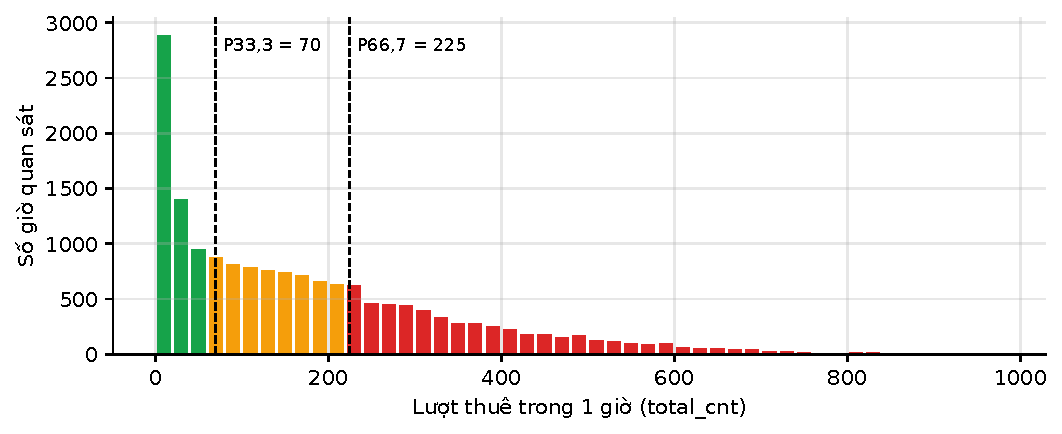
\includegraphics[width=0.95\textwidth]{figures/dss_distribution.pdf}
\caption{Phân phối lượt thuê theo giờ và hai ngưỡng phân loại}
\label{fig:dss-dist}
\end{figure}

\begin{table}[H]
\centering
\caption{Các phân vị của lượt thuê theo giờ (toàn bộ dữ liệu)}
\label{tab:percentiles}
\begin{tabular}{|c|c|c|c|c|c|c|c|c|}
\hline
\textbf{P10} & \textbf{P25} & \textbf{P33,3} & \textbf{P50} & \textbf{P66,7} & \textbf{P75} & \textbf{P90} & \textbf{TB} & \textbf{ĐLC} \\ \hline
9 & 40 & \textbf{70} & 142 & \textbf{225} & 281 & 451 & 189,5 & 181,4 \\ \hline
\end{tabular}
\end{table}
Với $\theta_L = 70$ và $\theta_H = 225$, tỷ lệ giờ quan sát rơi vào ba mức lần lượt là 33,1\%, 33,8\% và 33,1\% - đúng với mục tiêu chia đều.

\sect{Quy tắc ra quyết định và khuyến nghị}\label{sec:dss-rules}
\begin{table}[H]
\centering
\caption{Quy tắc ra quyết định (ngưỡng tính trên toàn bộ dữ liệu)}
\label{tab:rules}
\begin{tabularx}{\textwidth}{|c|p{3.2cm}|X|}
\hline
\textbf{Mức} & \textbf{Điều kiện} & \textbf{Khuyến nghị} \\ \hline
\Low & $\bar{y} < 70$ lượt/giờ & Duy trì mức chuẩn bị cơ bản. Có thể tận dụng khung giờ này để bảo trì, sửa chữa xe. \\ \hline
\Med & $70 \le \bar{y} \le 225$ & Theo dõi nhu cầu và duy trì nguồn lực phù hợp, sẵn sàng bổ sung nếu nhu cầu tăng. \\ \hline
\High & $\bar{y} > 225$ & Ưu tiên chuẩn bị thêm xe và nguồn lực phục vụ (nhân sự điều phối, hỗ trợ) trước khung giờ này. \\ \hline
-- & $n = 0$ & Không có dữ liệu lịch sử cho tình huống này, không đủ căn cứ để khuyến nghị. \\ \hline
\end{tabularx}
\end{table}

\subsect{Cảnh báo và danh sách ưu tiên}
Để trả lời câu hỏi ``khi nhu cầu dự kiến tăng cao, hệ thống cảnh báo gì'' (Q3.4), các giờ liên tiếp ở mức Cao được \textbf{gộp thành một khung cảnh báo}. Mỗi cảnh báo nêu: khoảng thời gian, giờ đỉnh và nhu cầu trung bình tại đỉnh, \textbf{thời điểm phải hoàn tất chuẩn bị} (một giờ trước khi khung bắt đầu). Các giờ Cao được sắp xếp giảm dần theo nhu cầu tạo thành \textbf{danh sách ưu tiên} (Q3.1). Ngoài ra, mỗi giờ có chỉ số \textit{so với trung bình kỳ} ($\bar{y}_{h,d,w} / \bar{y}$) để người vận hành hiểu mức độ chênh lệch.

\subsect{Nhóm khách cần phục vụ}\label{sec:dss-users}
Dữ liệu tách lượt thuê thành hai nhóm: \textbf{khách đăng ký} (thành viên, chủ yếu đi làm, đi học) và \textbf{khách vãng lai} (thuê lẻ, chủ yếu đi chơi, tham quan). Nhóm cân nhắc hai cách đưa thông tin này vào DSS:
\begin{itemize}
    \item \textit{Xếp mức riêng cho từng nhóm} (ngưỡng tính trên phân phối của nhóm đó): với khách vãng lai, ngưỡng Cao chỉ là 34 lượt/giờ nên gần như cả ban ngày (10--20h ngày làm việc, 9--21h ngày nghỉ) đều thành Cao - khuyến nghị mất khả năng phân biệt; với khách đăng ký (81\% lượt thuê), kết quả gần như trùng với cách xếp theo tổng.
    \item \textit{Giữ mức theo tổng, bổ sung thành phần khách} (\textbf{cách được chọn}): xe là tài sản dùng chung cho cả hai nhóm nên \textbf{số xe cần chuẩn bị} phụ thuộc tổng lượt thuê; còn \textbf{thành phần khách} quyết định \textbf{loại hỗ trợ} cần bố trí.
\end{itemize}
Gọi $c_{h,d,w}$ là tỷ lệ khách vãng lai của nhóm (tổng lượt vãng lai trung bình chia tổng lượt trung bình) và $\bar{c}$ là tỷ lệ vãng lai chung của kỳ lịch sử ($\bar{c} = 18{,}8\%$ trên toàn bộ dữ liệu). Mốc phân nhóm được đặt tương đối so với $\bar{c}$ nên tự điều chỉnh theo kỳ được chọn:
\[
\text{segment}(h,d,w) =
\begin{cases}
\text{Nhiều khách vãng lai} & \text{nếu } c_{h,d,w} \ge 1{,}5\,\bar{c} \quad (\ge 28{,}2\%)\\
\text{Chủ yếu khách đăng ký} & \text{nếu } c_{h,d,w} \le 0{,}75\,\bar{c} \quad (\le 14{,}1\%)\\
\text{Khách hỗn hợp} & \text{còn lại}
\end{cases}
\]
Tỷ lệ của một khung cảnh báo được tính có trọng số theo lượt thuê ($\sum$ vãng lai $/ \sum$ tổng của các giờ trong khung). Mỗi nhóm khách có một khuyến nghị bổ sung: \textit{chủ yếu đăng ký} - ưu tiên có đủ xe sẵn sàng đúng giờ, điều phối xe kịp thời; \textit{nhiều vãng lai} - bố trí nhân sự hướng dẫn thuê xe, hỗ trợ thanh toán và giải đáp cho khách mới; \textit{hỗn hợp} - kết hợp cả hai. Khuyến nghị này được ghép vào nội dung cảnh báo của khung.

\begin{lstlisting}[language=Python, caption={Phân loại và gộp khung cảnh báo (trích \code{src/dss/engine.py})}]
def classify(value, th):
    if value is None:
        return None                 # no historical data
    if value < th["low"]:
        return "low"
    if value > th["high"]:
        return "high"
    return "medium"

def high_windows(hours):            # hours: 24 items sorted by hour
    windows, cur = [], None
    for h in hours:
        if h["level"] == "high":
            if cur and h["hour"] == cur["end_hour"] + 1:
                cur["end_hour"] = h["hour"]; cur["hours"].append(h)
            else:
                cur = {"start_hour": h["hour"], "end_hour": h["hour"], "hours": [h]}
                windows.append(cur)
        else:
            cur = None
    return windows                  # + peak hour, prepare_before = start - 1
\end{lstlisting}

\subsect{Độ tin cậy}
Nhóm có ít hơn $n_{min} = 30$ giờ quan sát được gắn cờ \textit{độ tin cậy thấp} (hiển thị nhạt trên giao diện, kèm ghi chú); nhóm không có quan sát nào không được phân loại. Đây là cách DSS xử lý trung thực vấn đề dữ liệu thưa: mức thời tiết 4 chỉ có 3 giờ quan sát nên kịch bản ``ngày nghỉ, mưa lớn'' có 23/24 giờ không có dữ liệu, và hệ thống nói rõ điều đó thay vì suy diễn.

\sect{Kết quả của DSS}\label{sec:dss-results}
Hình~\ref{fig:dss-plan} là kế hoạch 24 giờ cho hai tình huống thường gặp nhất. Bảng~\ref{tab:scenarios} tóm tắt kết quả cho sáu tình huống có đủ dữ liệu.

\begin{figure}[H]
\centering
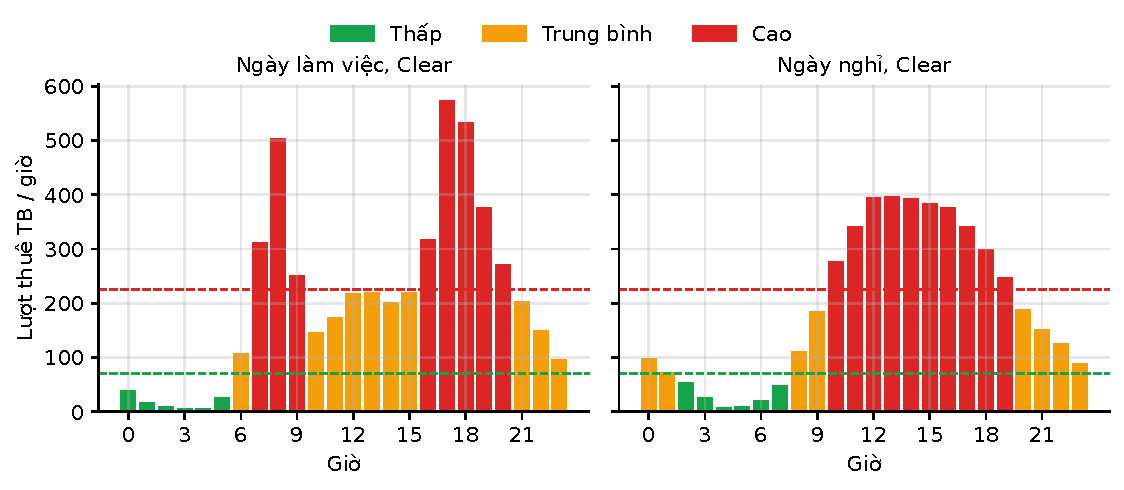
\includegraphics[width=\textwidth]{figures/dss_plan.pdf}
\caption{Mức nhu cầu dự kiến theo giờ: ngày làm việc và ngày nghỉ, trời quang (đường nét đứt: ngưỡng 70 và 225)}
\label{fig:dss-plan}
\end{figure}

\begin{table}[H]
\centering
\caption{Kết quả DSS theo tình huống (ngưỡng P33,3/P66,7, toàn bộ dữ liệu)}
\label{tab:scenarios}
\small
\begin{tabularx}{\textwidth}{|l|l|c|c|c|X|p{2.6cm}|}
\hline
\textbf{Loại ngày} & \textbf{Thời tiết} & \textbf{Thấp} & \textbf{TB} & \textbf{Cao} & \textbf{Khung cảnh báo} & \textbf{Nhóm khách (\% vãng lai)} \\ \hline
Làm việc & Clear & 6 & 10 & 8 & 07:00--09:59 (đỉnh 8h, 504); 16:00--20:59 (đỉnh 17h, 574) & Chủ yếu đăng ký (5,9\%; 12,5\%) \\ \hline
Làm việc & Mist & 6 & 11 & 7 & 07:00--09:59; 16:00--19:59 & Chủ yếu đăng ký (5,8\%; 10,5\%) \\ \hline
Làm việc & Light rain/snow & 8 & 13 & 3 & 08:00--08:59; 17:00--18:59 & Chủ yếu đăng ký (3,9\%; 8,9\%) \\ \hline
Nghỉ & Clear & 6 & 8 & 10 & 10:00--19:59 (đỉnh 12--13h, 396) & Nhiều vãng lai (35,4\%) \\ \hline
Nghỉ & Mist & 7 & 8 & 9 & 10:00--18:59 & Nhiều vãng lai (32,9\%) \\ \hline
Nghỉ & Light rain/snow & 11 & 11 & 2 & 12:00--12:59; 15:00--15:59 (ít mẫu) & Nhiều vãng lai (35,3\%; 32,8\%) \\ \hline
\end{tabularx}
\end{table}

\noindent Ngoài hai nhóm ngày, người dùng có thể chọn \textbf{một hoặc nhiều thứ cụ thể} (ví dụ chỉ thứ sáu, hoặc thứ hai + thứ ba): hệ thống lấy các ngày thuộc các thứ đó \textit{không phải ngày lễ} (ngày lễ thuộc nhóm ngày nghỉ). Khi chọn từ hai thứ trở lên, có hai cách tính:
\begin{itemize}
    \item \textbf{Từng thứ riêng} (mặc định): mỗi thứ được lập một kế hoạch riêng (trung bình theo giờ của riêng thứ đó) và các kế hoạch được đặt cạnh nhau để so sánh - mỗi thứ có khung cao điểm, giờ phải chuẩn bị xong và nhóm khách của riêng nó (Hình~\ref{fig:dash-dss-compare}). Đây là cách phù hợp khi cần chuẩn bị cho nhiều ngày sắp tới, ví dụ thứ sáu và thứ bảy.
    \item \textbf{Gộp thành một kế hoạch}: các ngày của mọi thứ đã chọn được gộp và lấy trung bình chung theo giờ. Cách này chỉ nên dùng khi các thứ có dạng nhu cầu giống nhau (ví dụ thứ hai + thứ ba, hoặc thứ bảy + chủ nhật) để có thêm dữ liệu, nhất là khi trời mưa hoặc sương mù. Nếu gộp lẫn ngày trong tuần với cuối tuần, kết quả là một đường ``trung bình'' không giống ngày nào (ví dụ thứ tư + thứ bảy: 8h thành Cao với 297 lượt/giờ, trong khi riêng thứ bảy 8h chỉ 125 lượt/giờ - mức Trung bình), nên giao diện hiện cảnh báo đề nghị chọn \textit{Từng thứ riêng}.
\end{itemize}
Trong dữ liệu, cả 21 ngày lễ đều rơi vào thứ hai đến thứ sáu (15 ngày vào thứ hai), nên điều kiện này chỉ có tác dụng với các ngày trong tuần; khi chọn thứ bảy, chủ nhật, giao diện không hiện ghi chú về ngày lễ. Chọn đủ thứ hai đến thứ sáu cho kết quả trùng với nhóm ``ngày làm việc'' (đã được kiểm thử), nên đây là cách tổng quát hóa của nhóm ngày. Ví dụ thứ hai + thứ ba, trời quang: 8 giờ Cao trong hai khung 07:00--09:59 và 16:00--20:59, đỉnh 17h (578 lượt/giờ), 13,5\% khách vãng lai (chủ yếu khách đăng ký). Mỗi thứ có khoảng 100 ngày lịch sử nên với trời quang mỗi giờ vẫn có 44--66 quan sát (đủ ngưỡng tin cậy 30); với sương mù hoặc mưa, nhiều giờ sẽ bị gắn cờ ít dữ liệu. Bảng~\ref{tab:weekdays} cho thấy việc chọn theo thứ giúp phát hiện khác biệt mà nhóm ``ngày làm việc'' che mất.

\begin{table}[H]
\centering
\caption{Kết quả DSS theo từng thứ trong tuần (trời quang, toàn bộ dữ liệu)}
\label{tab:weekdays}
\small
\begin{tabularx}{\textwidth}{|l|c|c|c|c|X|}
\hline
\textbf{Thứ} & \textbf{Thấp} & \textbf{TB} & \textbf{Cao} & \textbf{Giờ đỉnh} & \textbf{Khung cảnh báo (chuẩn bị trước; nhóm khách, \% vãng lai)} \\ \hline
Thứ hai & 6 & 10 & 8 & 17h (572) & 07:00--09:59 (06:00; đăng ký, 6,4\%); 16:00--20:59 (15:00; đăng ký, 12,1\%) \\ \hline
Thứ ba & 6 & 10 & 8 & 17h (582) & 07:00--09:59; 16:00--20:59 (đăng ký) \\ \hline
Thứ tư & 6 & 10 & 8 & 17h (595) & 07:00--09:59; 16:00--20:59 (đăng ký) \\ \hline
Thứ năm & 6 & 10 & 8 & 17h (593) & 07:00--09:59; 16:00--20:59 (đăng ký) \\ \hline
Thứ sáu & 6 & 6 & \textbf{12} & 17h (525) & 07:00--09:59 (06:00; đăng ký, 6,4\%); \textbf{12:00--20:59} (11:00; hỗn hợp, 19,1\%) \\ \hline
Thứ bảy & 6 & 8 & 10 & 12h (429) & 10:00--19:59 (09:00; nhiều vãng lai, 36,6\%) \\ \hline
Chủ nhật & 7 & 7 & 10 & 14h (387) & 10:00--19:59 (09:00; nhiều vãng lai, 34,9\%) \\ \hline
\end{tabularx}
\end{table}

\noindent Nhận xét:
\begin{itemize}
    \item \textbf{Ngày làm việc} có hai khung cao điểm tách biệt, ứng với giờ đi làm và tan tầm; khung chiều dài hơn và cao hơn (đỉnh 574 lượt/giờ lúc 17h). Khung trưa 10--15h chỉ ở mức Trung bình: phù hợp để điều phối lại xe giữa hai đợt cao điểm.
    \item \textbf{Ngày nghỉ} có một khung cao điểm liền mạch 10--19h (nhu cầu giải trí), buổi sáng sớm ở mức Thấp: không cần chuẩn bị sớm như ngày làm việc.
    \item \textbf{Thời tiết}: trời sương mù chỉ làm giảm nhẹ (khung cảnh báo gần như giữ nguyên), nhưng mưa/tuyết nhẹ làm số giờ Cao giảm từ 8 xuống 3 (ngày làm việc) và từ 10 xuống 2 (ngày nghỉ). Dù vậy giờ 8h và 17--18h của ngày làm việc vẫn Cao khi mưa nhẹ: nhu cầu đi làm ít co giãn theo thời tiết.
    \item \textbf{Nhóm khách}: cùng là mức Cao nhưng cần chuẩn bị khác nhau. Cao điểm ngày làm việc gần như toàn khách đăng ký (vãng lai chỉ 4--13\%): trọng tâm là đủ xe đúng giờ đi làm, tan tầm. Cao điểm ngày nghỉ có hơn 1/3 lượt thuê là khách vãng lai: cần thêm nhân sự hướng dẫn, hỗ trợ thanh toán cho khách mới.
    \item \textbf{Theo thứ}: thứ hai đến thứ năm gần như giống nhau, nhưng \textbf{thứ sáu} có khung cao buổi chiều bắt đầu sớm từ 12h (cần chuẩn bị trước 11:00 thay vì 15:00) với tỷ lệ khách vãng lai cao hơn (hỗn hợp, 19,1\%); thứ bảy có nhu cầu đỉnh cao hơn chủ nhật (429 so với 387 lượt/giờ). Gộp chung ``ngày làm việc'' sẽ bỏ sót đặc điểm của thứ sáu.
    \item \textbf{Khung giờ thấp} (0--5h) ổn định ở mức Thấp trong mọi tình huống: thời điểm phù hợp để bảo trì, sạc, thu hồi xe hỏng.
\end{itemize}

\begin{figure}[H]
\centering
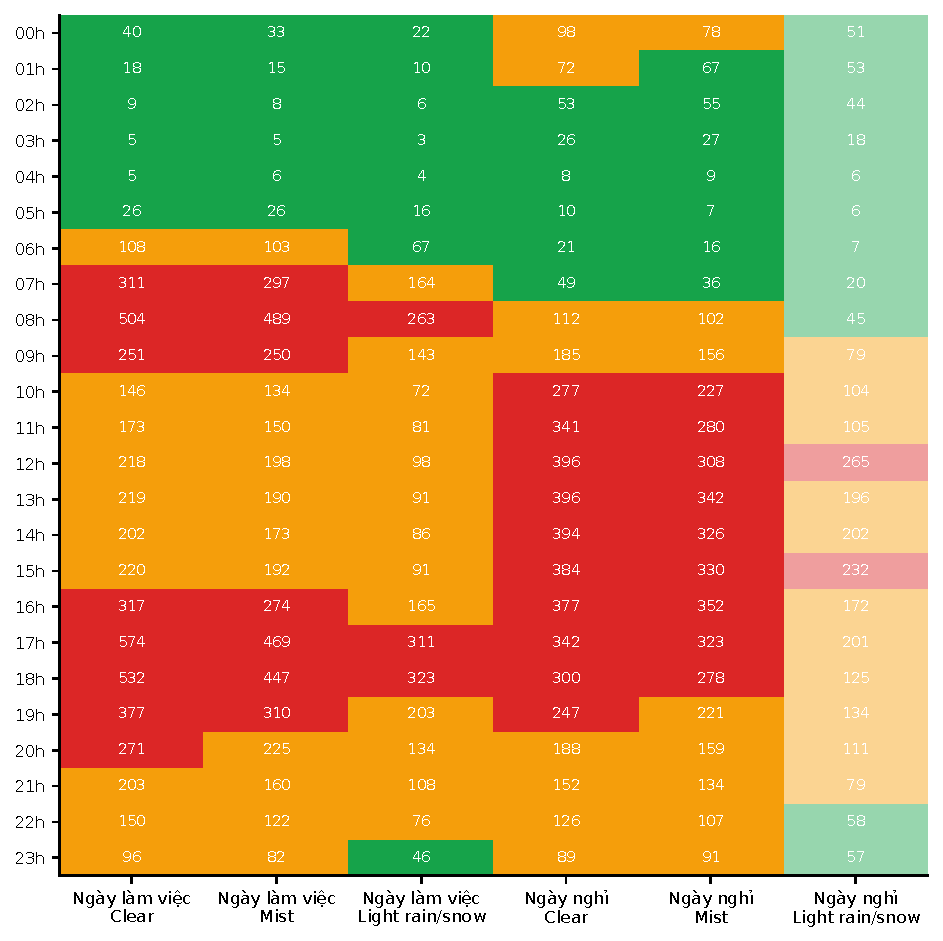
\includegraphics[width=0.82\textwidth]{figures/dss_matrix.pdf}
\caption{Ma trận phân loại giờ $\times$ loại ngày $\times$ thời tiết (số trong ô: lượt thuê TB/giờ; ô nhạt: dưới 30 giờ quan sát; bỏ cột mưa lớn do gần như không có dữ liệu)}
\label{fig:dss-matrix}
\end{figure}

\sect{Phân tích độ nhạy}\label{sec:dss-sensitivity}
Một đặc tính quan trọng của DSS là cho phép người dùng thay đổi giả định và quan sát ảnh hưởng (phân tích ``what-if''). Nhóm thử hai loại thay đổi trên tình huống ``ngày làm việc, trời quang'':

\begin{table}[H]
\centering
\caption{Phân tích độ nhạy của kết quả phân loại}
\label{tab:sensitivity}
\begin{tabularx}{\textwidth}{|p{4.6cm}|c|c|c|X|}
\hline
\textbf{Cấu hình} & \textbf{$\theta_L$} & \textbf{$\theta_H$} & \textbf{Số giờ Cao} & \textbf{Khung cảnh báo} \\ \hline
P33,3/P66,7, toàn bộ dữ liệu (mặc định) & 70 & 225 & 8 & 07--09h; 16--20h \\ \hline
P25/P75, toàn bộ dữ liệu & 40 & 281 & 6 & 07--08h; 16--19h \\ \hline
P33,3/P66,7, kỳ lịch sử 2012 & 98 & 284 & 8 & 07--09h; 16--20h \\ \hline
\end{tabularx}
\end{table}
Ngưỡng chặt hơn (P75) chỉ loại bớt giờ ``rìa'' của khung (9h và 20h), còn lõi cao điểm 7--8h và 16--19h không đổi. Khi chỉ dùng dữ liệu 2012 (nhu cầu cao hơn 2011 khoảng 65\%), ngưỡng tăng tương ứng nhưng các khung cảnh báo giữ nguyên. Kết luận: \textbf{các khung giờ ưu tiên là ổn định}, không phải hệ quả của việc chọn ngưỡng - tăng độ tin cậy của khuyến nghị.

\sect{Giao diện DSS}\label{sec:dss-ui}
Giao diện DSS nằm ở trang riêng ``Hỗ trợ quyết định'' của dashboard (\code{\#/dss}, Hình~\ref{fig:dash-dss-top}--\ref{fig:dash-dss-matrix}). Trang được thiết kế cho \textbf{người vận hành} (không cần hiểu thống kê) theo luồng đánh số từng bước, đi từ câu hỏi tới hành động:
\begin{enumerate}
    \item \textbf{Chọn tình huống sắp tới}: hai nhóm nút bấm lớn có mô tả ngắn - loại ngày (Ngày làm việc / Ngày nghỉ, \textit{hoặc} một / nhiều thứ cụ thể bằng hàng nút T2 \ldots{} CN bấm bật / tắt, có nút bỏ chọn; khi chọn từ hai thứ có thêm lựa chọn \textit{Từng thứ riêng} / \textit{Gộp thành 1 kế hoạch}) và thời tiết dự báo (Quang đãng, Sương mù, Mưa nhẹ, Mưa lớn). Kỳ lịch sử lấy từ bộ lọc dropdown Năm/Mùa (trang này chỉ hiện hai bộ lọc đó) và được nhắc lại bằng chữ ngay dưới các nút.
    \item \textbf{Kết luận}: một câu tóm tắt (ví dụ ``Có 2 khung giờ cao điểm. Cần chuẩn bị xong trước 06:00 và 15:00''), kèm số giờ ở mỗi mức, giờ đông nhất và nhãn nhóm khách của cả tình huống (ví dụ ``Nhiều khách vãng lai - 32,4\% lượt thuê, mức chung 18,8\%''). Khi tình huống hiếm gặp (đa số giờ không có hoặc có ít dữ liệu, như trời mưa lớn), hệ thống hiện cảnh báo \textit{không đủ dữ liệu để kết luận chắc chắn} thay vì đưa ra khuyến nghị gây hiểu nhầm.
    \item \textbf{Việc cần làm}: mỗi khung cảnh báo là một thẻ với mốc thời gian \textit{hoàn tất trước} nổi bật, khung giờ cao điểm, giờ đỉnh và lượt thuê trung bình, cùng nhãn nhóm khách của khung (kèm \% vãng lai) và khuyến nghị loại hỗ trợ tương ứng (Hình~\ref{fig:dash-dss-weekend}).
    \item \textbf{24 giờ trong ngày}: dải 24 ô tô màu theo mức để nhìn nhanh cả ngày, biểu đồ cột với hai đường ngưỡng, và ba thẻ giải thích ngưỡng cùng khuyến nghị của từng mức.
    \item \textbf{Nhóm khách cần phục vụ} (Hình~\ref{fig:dash-dss-users}): biểu đồ cột chồng lượt thuê của khách đăng ký và vãng lai theo giờ, dải 24 ô tô màu theo nhóm khách, giải thích mốc phân nhóm (tính theo tỷ lệ chung của kỳ) và ba thẻ khuyến nghị theo nhóm khách.
\end{enumerate}
Ở chế độ \textit{Từng thứ riêng} (Hình~\ref{fig:dash-dss-compare}), các bước trên được trình bày dạng so sánh: mỗi thứ một thẻ kết luận; việc cần làm nhóm theo từng thứ; các dải 24 ô xếp chồng (mỗi thứ một hàng) cùng biểu đồ đường, mỗi đường là một thứ; dải nhóm khách cũng xếp theo từng thứ; phần chi tiết có bảng so sánh từng giờ giữa các thứ.
Phần dành cho người phân tích được \textbf{thu gọn mặc định} (mở khi cần): bảng chi tiết từng giờ (nhu cầu, hệ số so với trung bình, số giờ quan sát, tỷ lệ khách vãng lai, nhóm khách, mức, khuyến nghị); giải thích cách xác định ngưỡng kèm bảng khảo sát phân phối và lựa chọn cách chia ngưỡng (phân tích độ nhạy); ma trận phân loại cho mọi tình huống.

\begin{figure}[H]
\centering
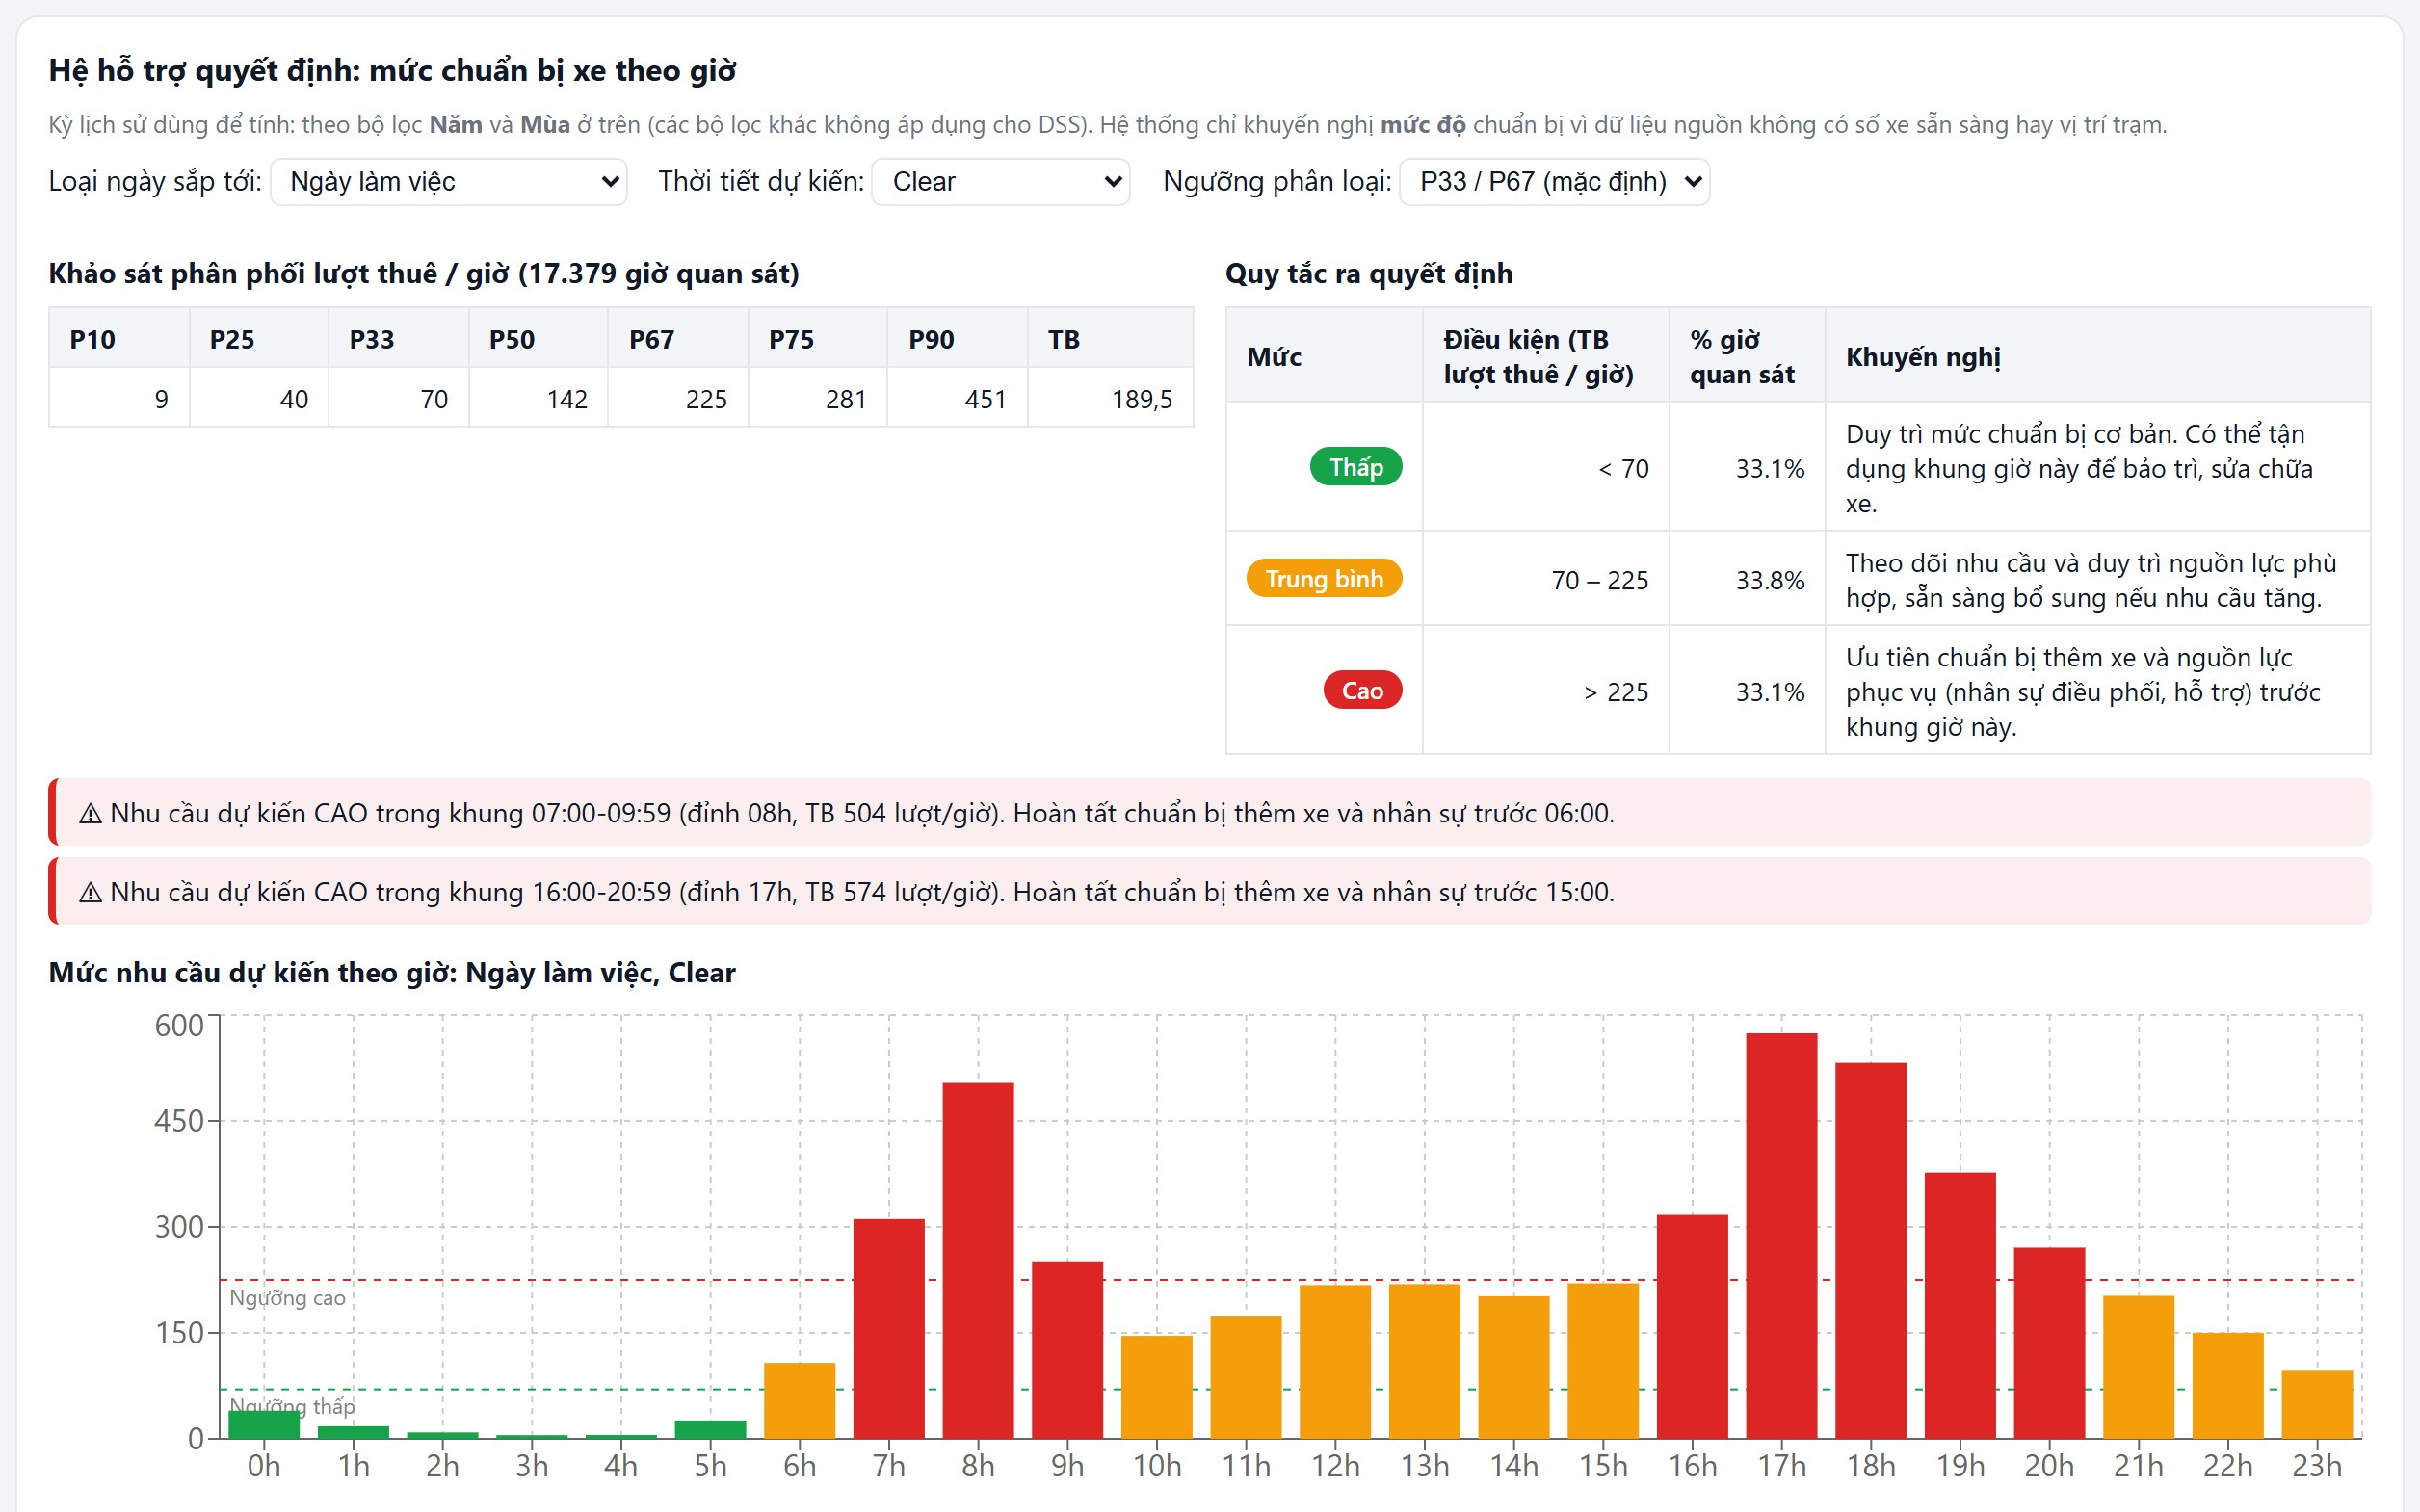
\includegraphics[width=0.85\textwidth]{figures/dash_dss_top.jpg}
\caption{Giao diện DSS: chọn tình huống, kết luận, việc cần làm và mức nhu cầu 24 giờ (ngày làm việc, trời quang đãng)}
\label{fig:dash-dss-top}
\end{figure}

\begin{figure}[H]
\centering
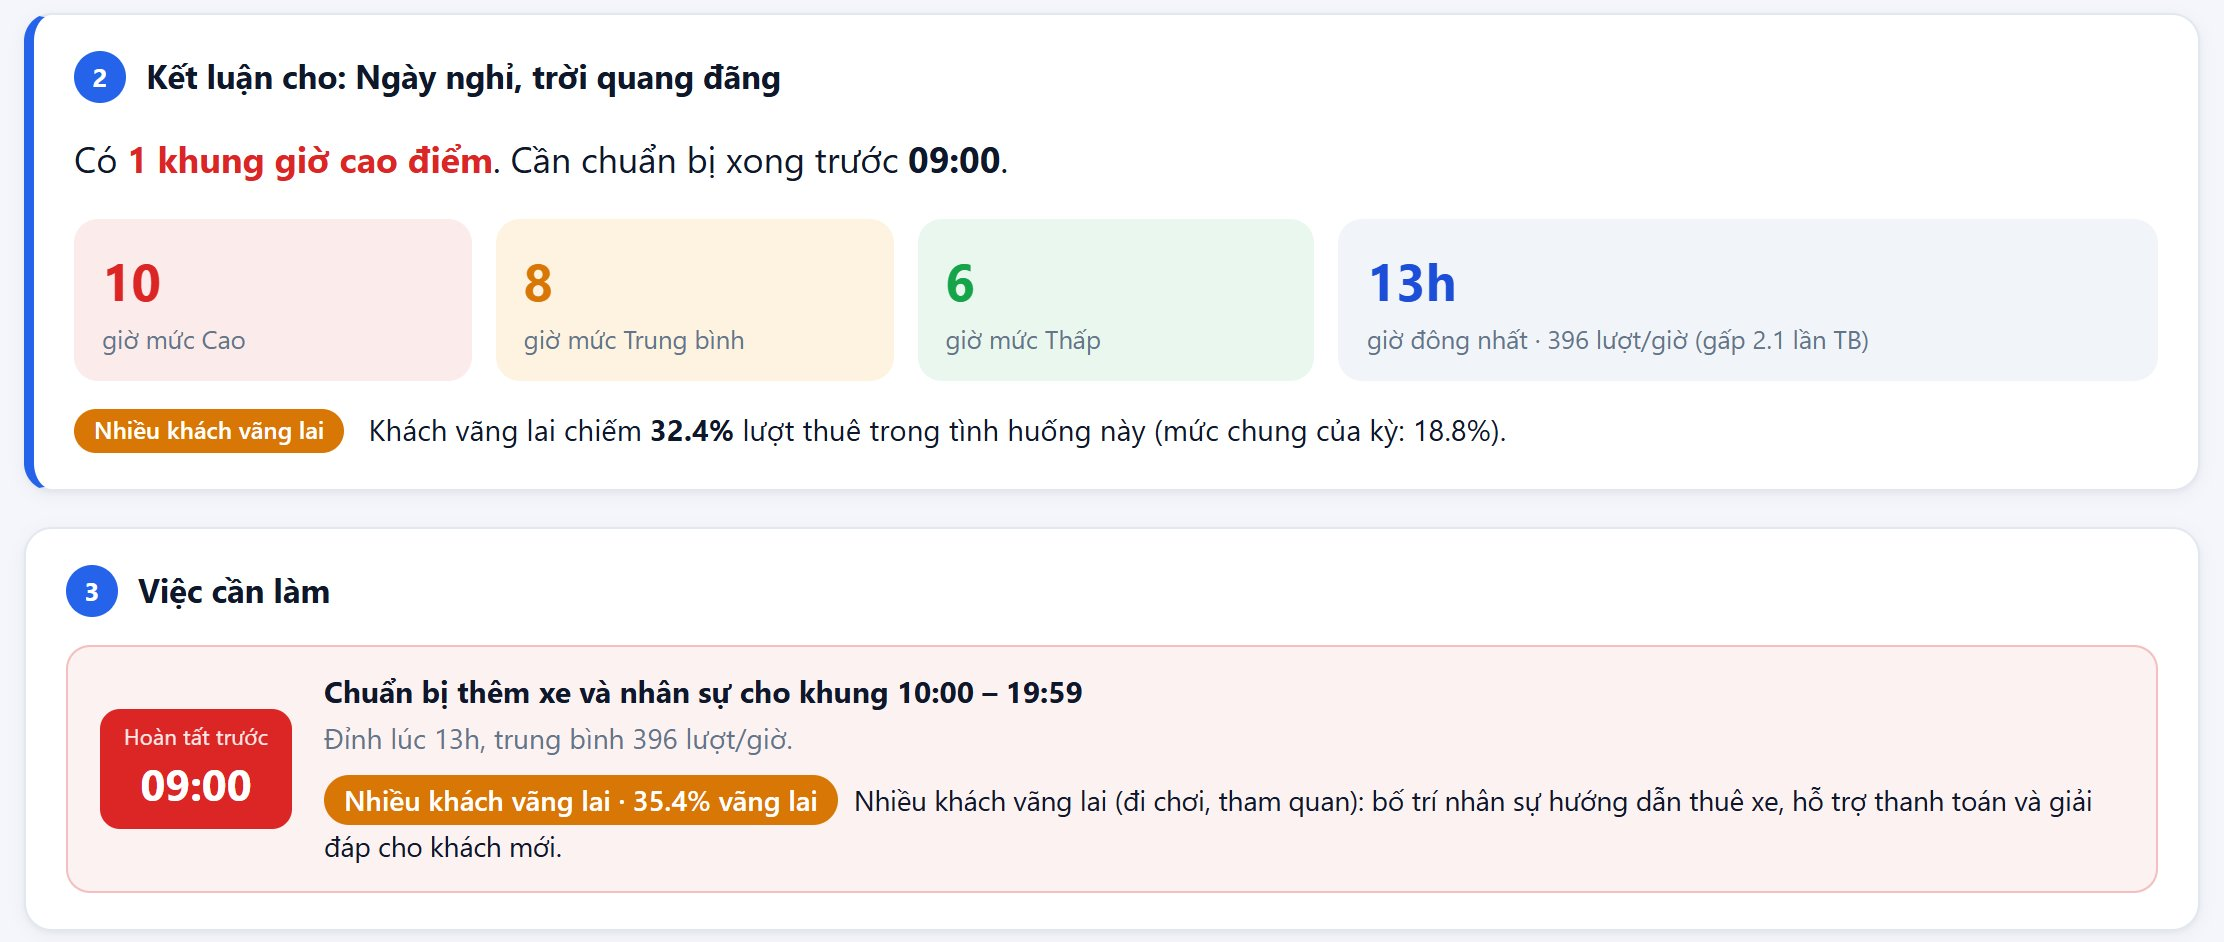
\includegraphics[width=0.9\textwidth]{figures/dash_dss_weekend.jpg}
\caption{Giao diện DSS với tình huống ngày nghỉ, trời quang đãng: kết luận và việc cần làm kèm nhóm khách (nhiều khách vãng lai)}
\label{fig:dash-dss-weekend}
\end{figure}

\begin{figure}[H]
\centering
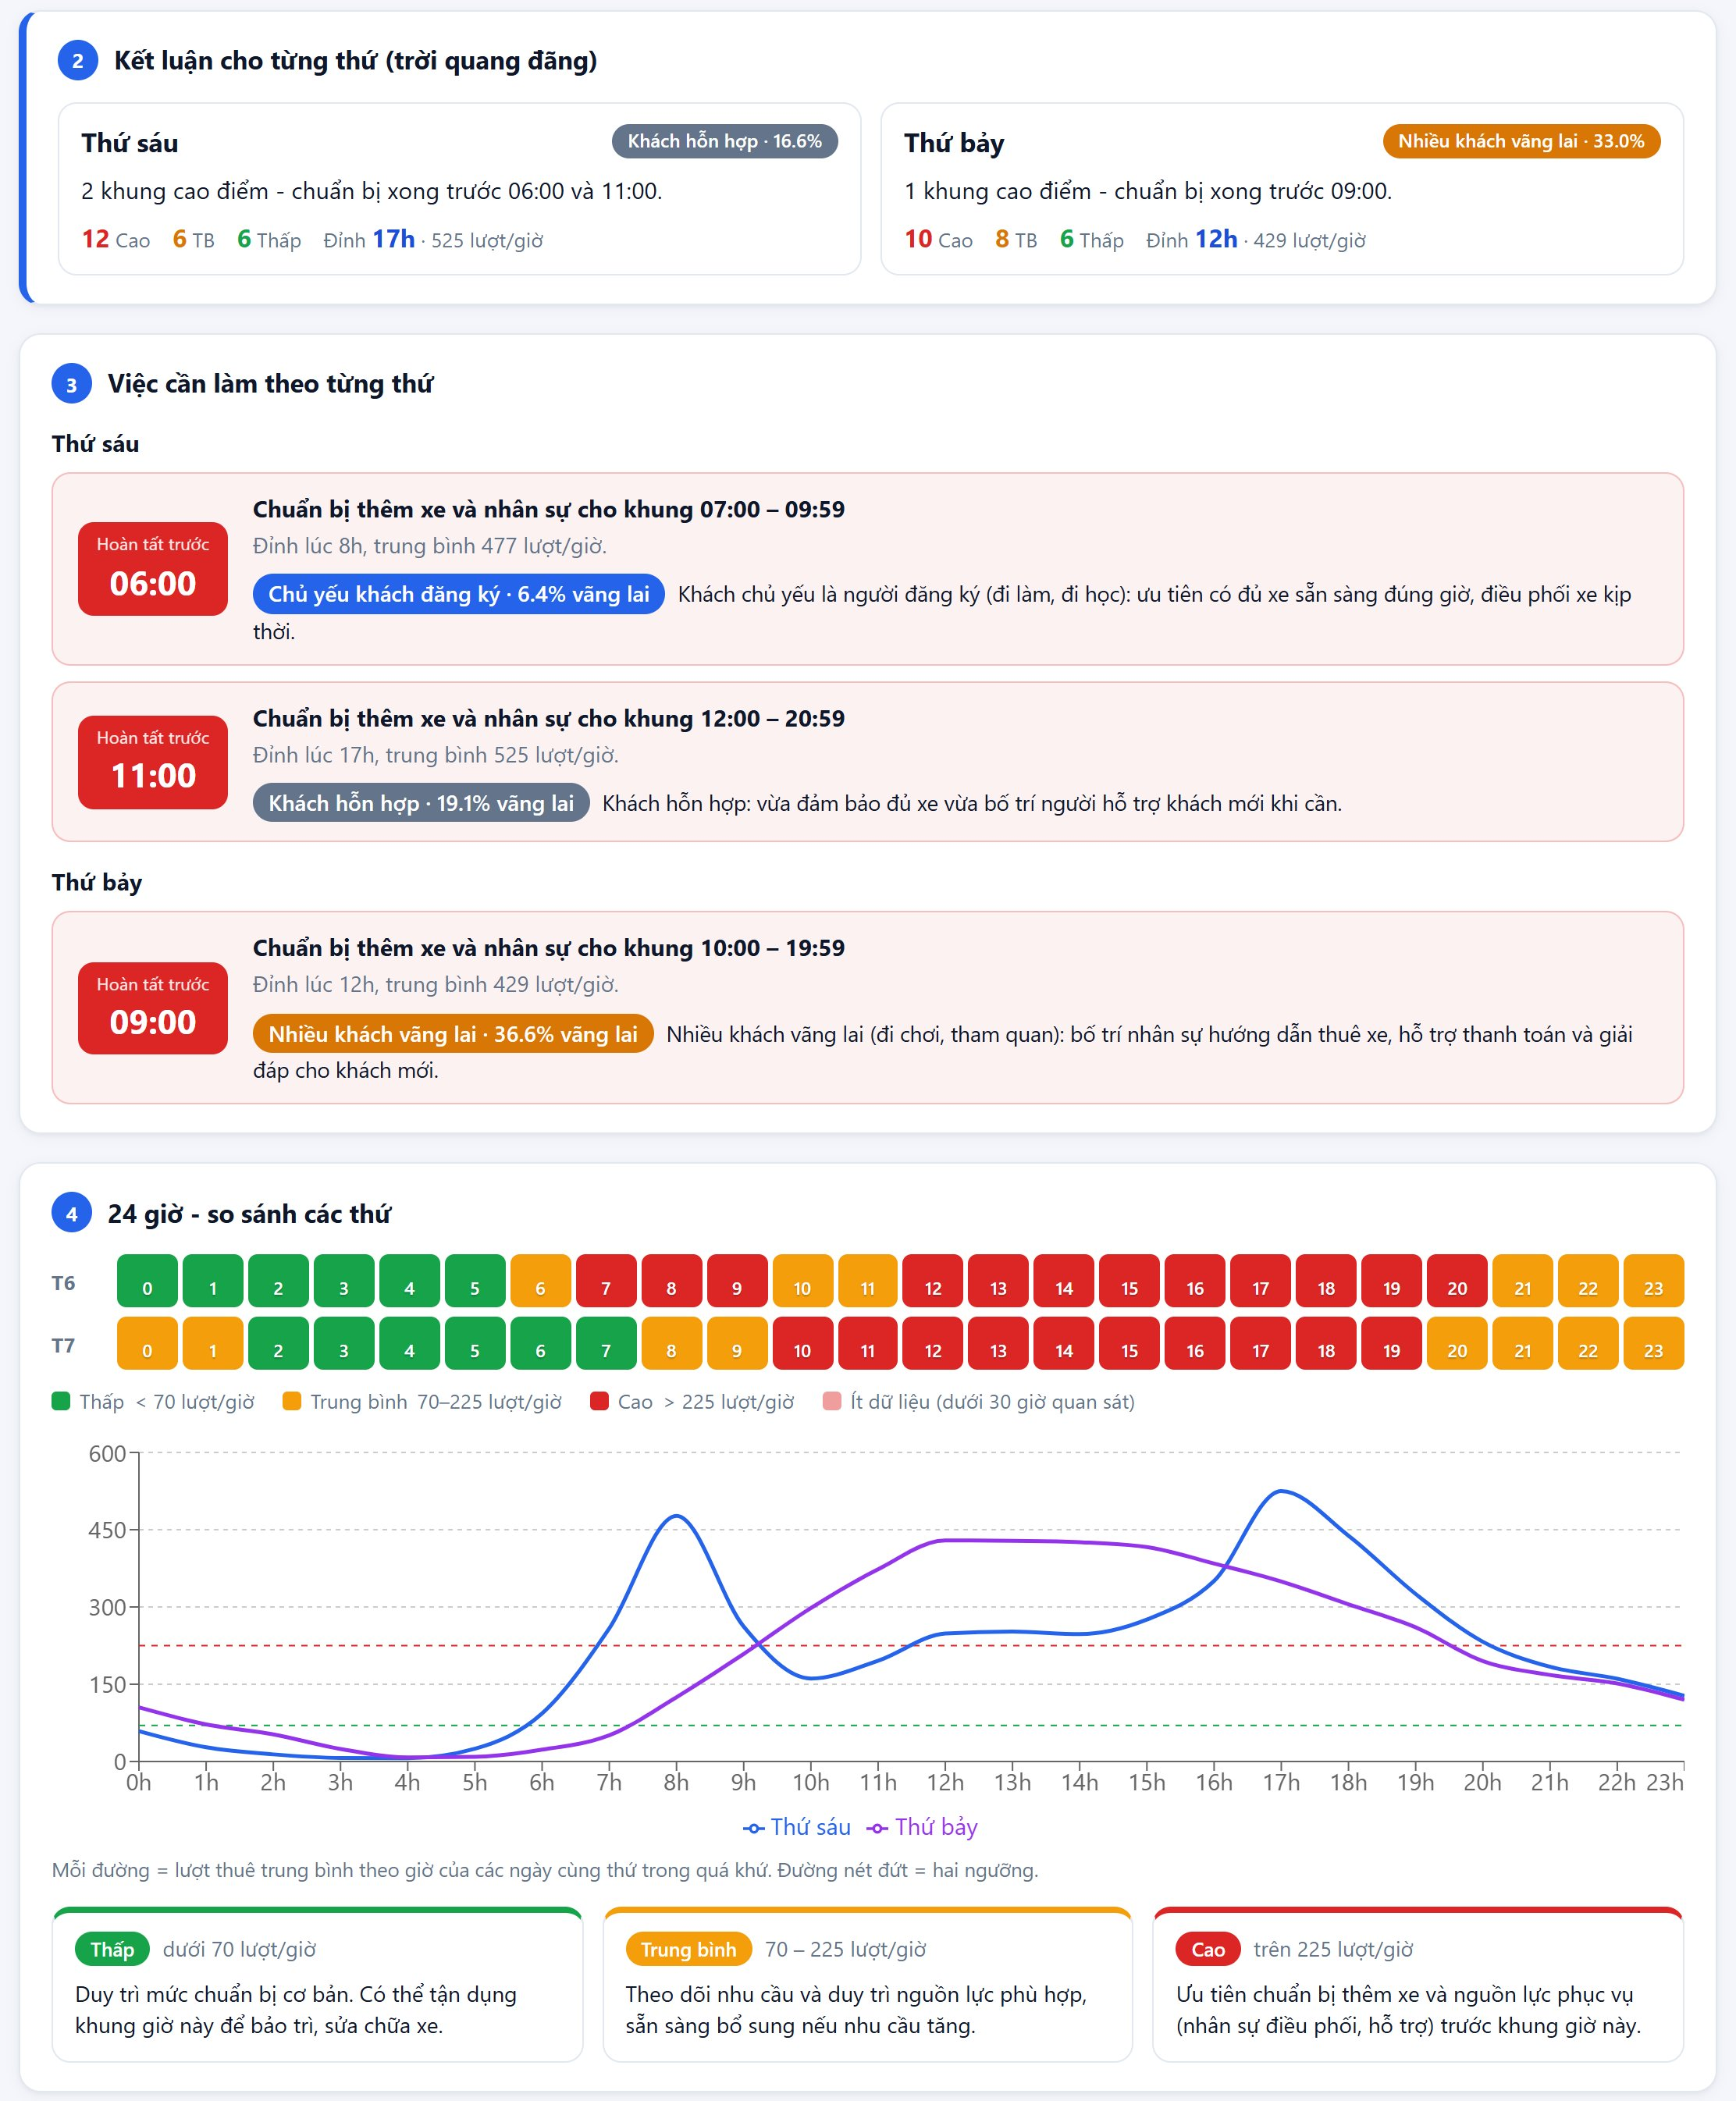
\includegraphics[width=0.8\textwidth]{figures/dash_dss_compare.jpg}
\caption{Giao diện DSS khi chọn thứ sáu và thứ bảy (chế độ \textit{Từng thứ riêng}): kết luận, việc cần làm và mức nhu cầu 24 giờ của từng thứ}
\label{fig:dash-dss-compare}
\end{figure}

\begin{figure}[H]
\centering
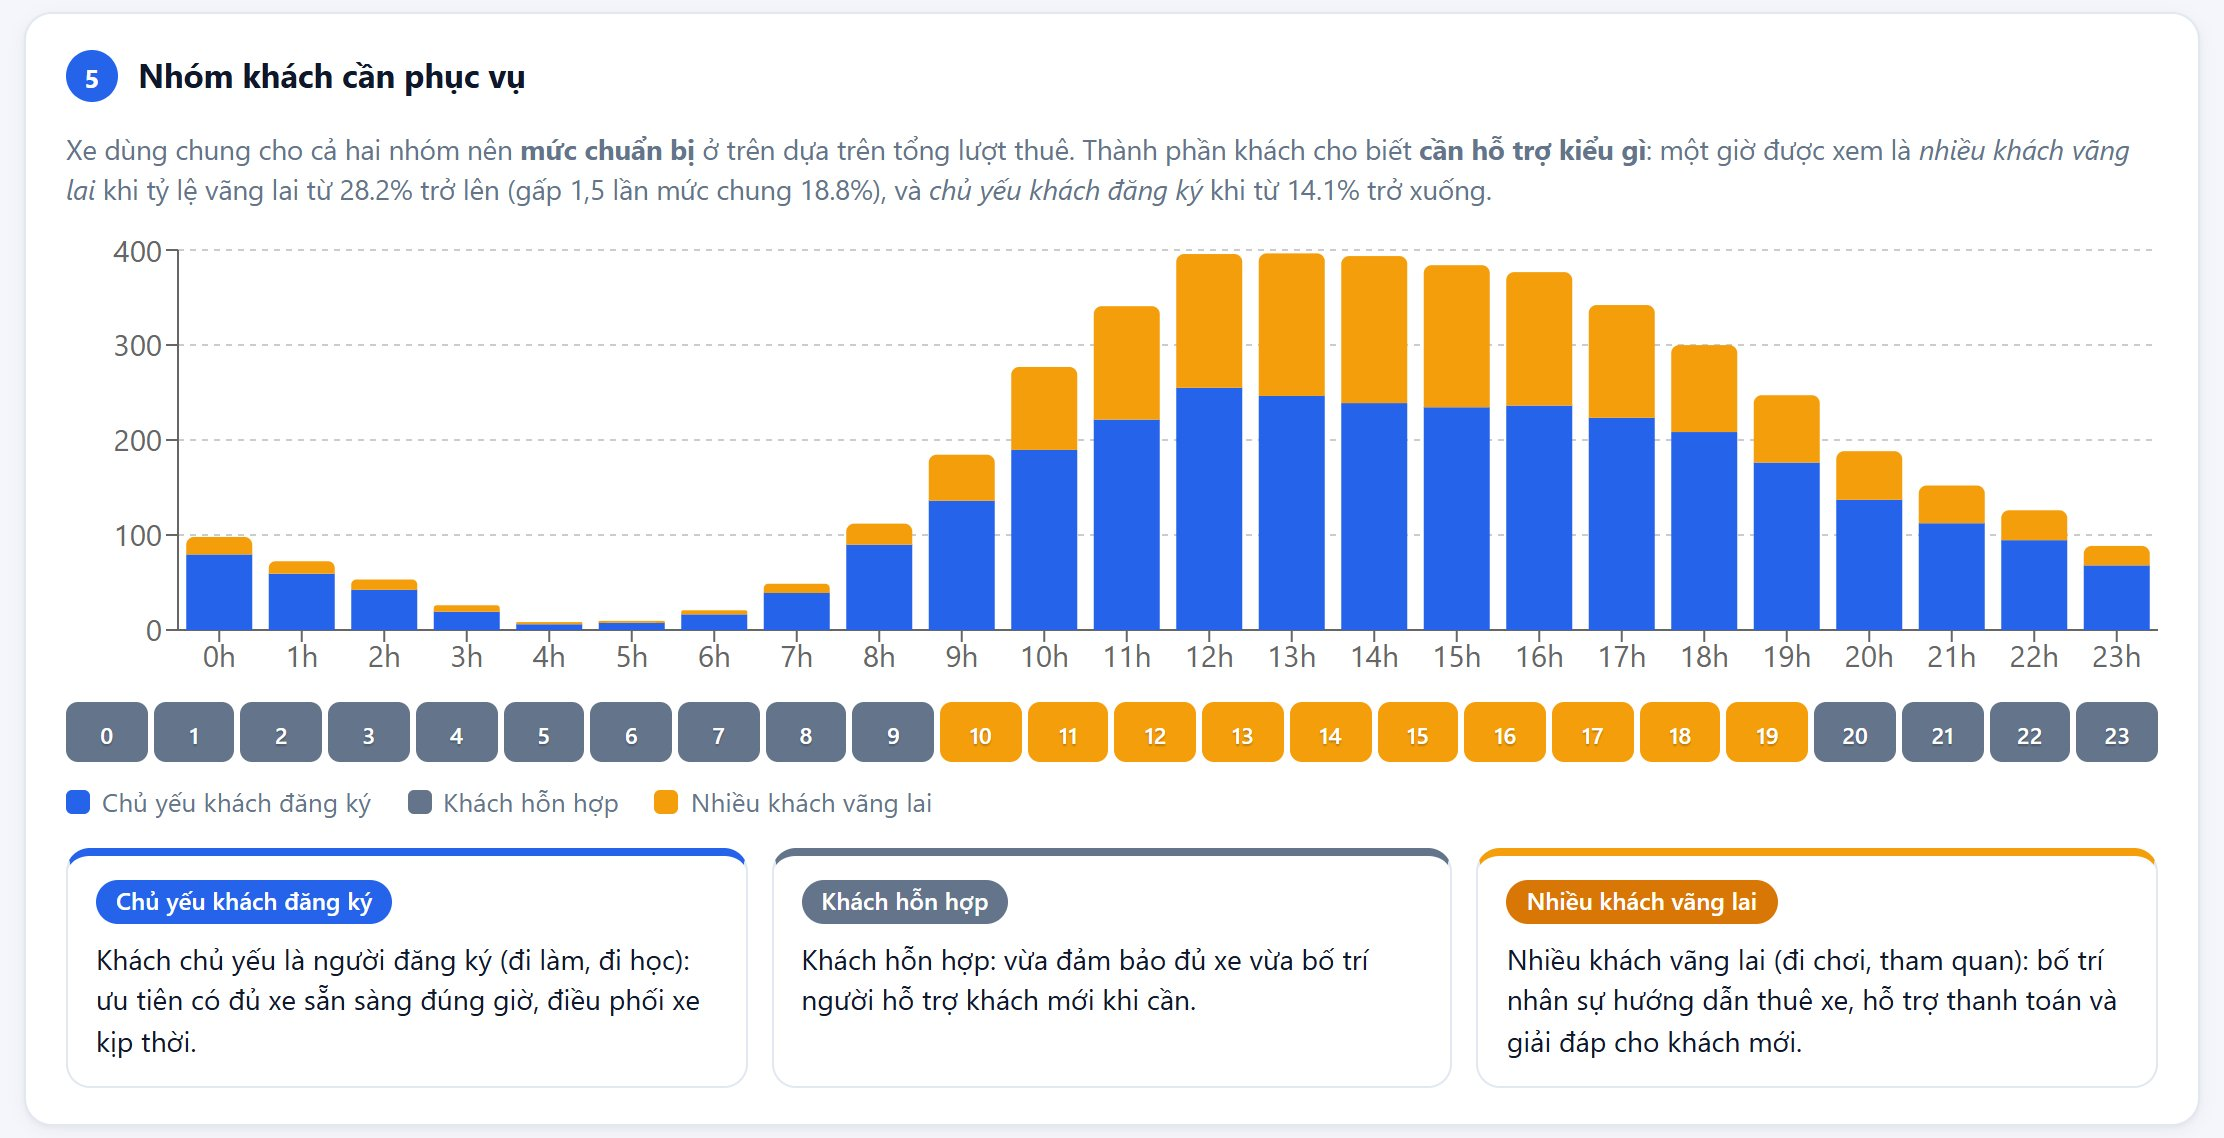
\includegraphics[width=0.9\textwidth]{figures/dash_dss_users.jpg}
\caption{Giao diện DSS: thành phần khách theo giờ và khuyến nghị theo nhóm khách (ngày nghỉ, trời quang đãng)}
\label{fig:dash-dss-users}
\end{figure}

\begin{figure}[H]
\centering
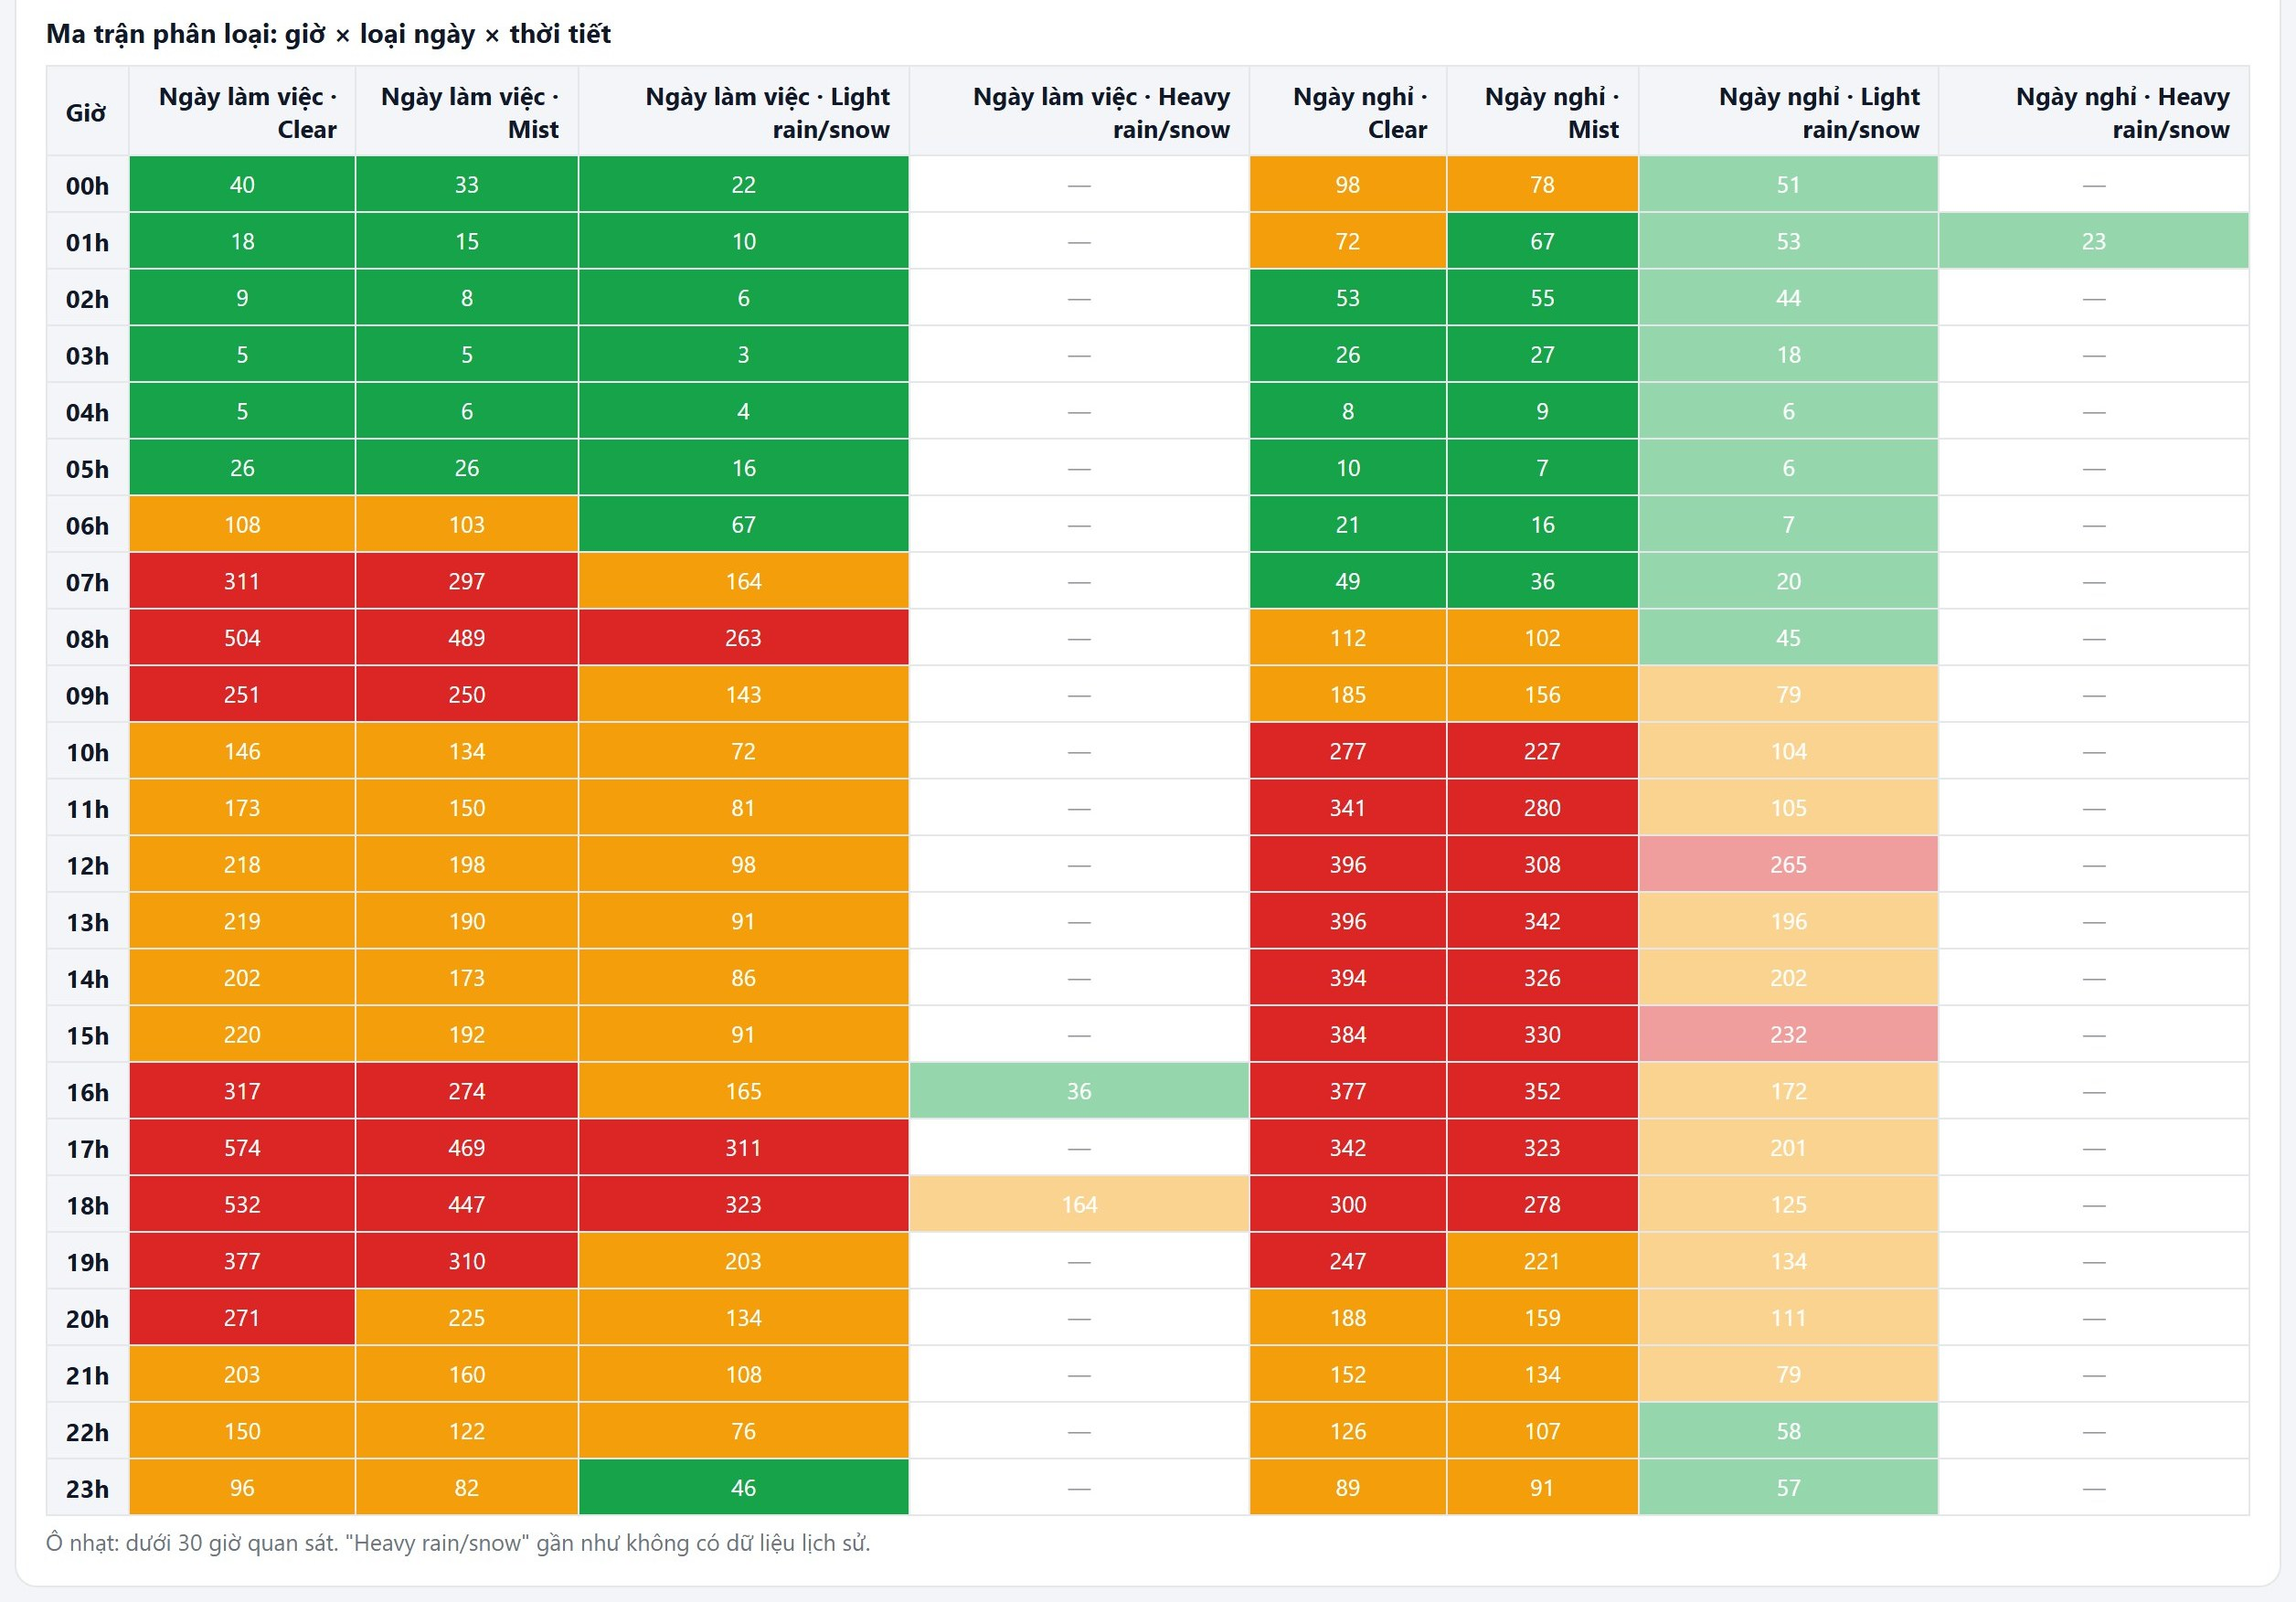
\includegraphics[width=0.92\textwidth]{figures/dash_dss_matrix.jpg}
\caption{Giao diện DSS: ma trận phân loại giờ $\times$ loại ngày $\times$ thời tiết (phần chi tiết, mở khi cần)}
\label{fig:dash-dss-matrix}
\end{figure}

% ==================== CHƯƠNG 9 ====================
\newpage
\chap{Kết quả phân tích: trả lời các câu hỏi nghiệp vụ}\label{sec:results}
Mục này dùng kho dữ liệu và dashboard để trả lời các câu hỏi ở mục~\ref{sec:questions}. Tất cả số liệu được truy vấn từ kho \code{dw} (toàn bộ 2011--2012 nếu không ghi khác); các hình được sinh tự động bằng \code{report/scripts/make\_figures.py}.

\sect{Nhóm 1 - Phân tích nhu cầu sử dụng}

\noindent\textbf{Q1.1 - Tổng lượt thuê.} Hai năm có \textbf{3.292.679} lượt thuê (17.379 giờ, 731 ngày), trung bình 189,5 lượt/giờ. Năm 2011 có 1.243.103 lượt, năm 2012 có 2.049.576 lượt - \textbf{tăng 64,9\%}, cho thấy hệ thống đang tăng trưởng mạnh; điều này cũng là lý do DSS cho phép chọn kỳ lịch sử gần nhất.

\begin{table}[H]
\centering
\caption{Tám KPI trên toàn bộ dữ liệu}
\label{tab:kpi-values}
\begin{tabular}{|l|r|l|}
\hline
\textbf{KPI} & \textbf{Giá trị} & \textbf{Ghi chú} \\ \hline
Total Rentals & 3.292.679 & 2011: 1.243.103; 2012: 2.049.576 \\ \hline
Average Hourly Rentals & 189,5 & lượt/giờ \\ \hline
Peak Hour & 17h & TB 461,5 lượt/giờ \\ \hline
Lowest Demand Hour & 4h & TB 6,4 lượt/giờ \\ \hline
Registered User Ratio & 81,2\% & 2.672.662 lượt \\ \hline
Casual User Ratio & 18,8\% & 620.017 lượt \\ \hline
Working Day Demand & 4.585 & lượt/ngày (500 ngày) \\ \hline
Non-working Day Demand & 4.330 & lượt/ngày (231 ngày) \\ \hline
\end{tabular}
\end{table}

\noindent\textbf{Q1.2 - Khung giờ cao nhất và thấp nhất.} Trên toàn bộ dữ liệu, giờ cao điểm là \textbf{17h} (461,5 lượt/giờ) và giờ thấp nhất là \textbf{4h} (6,4 lượt/giờ) - chênh lệch hơn 70 lần. Hình~\ref{fig:hourly} cho thấy hồ sơ theo giờ khác hẳn giữa hai loại ngày: ngày làm việc có hai đỉnh nhọn lúc 8h (477) và 17h (525); ngày nghỉ có một đỉnh tròn lúc 12--14h (khoảng 370).

\begin{figure}[H]
\centering
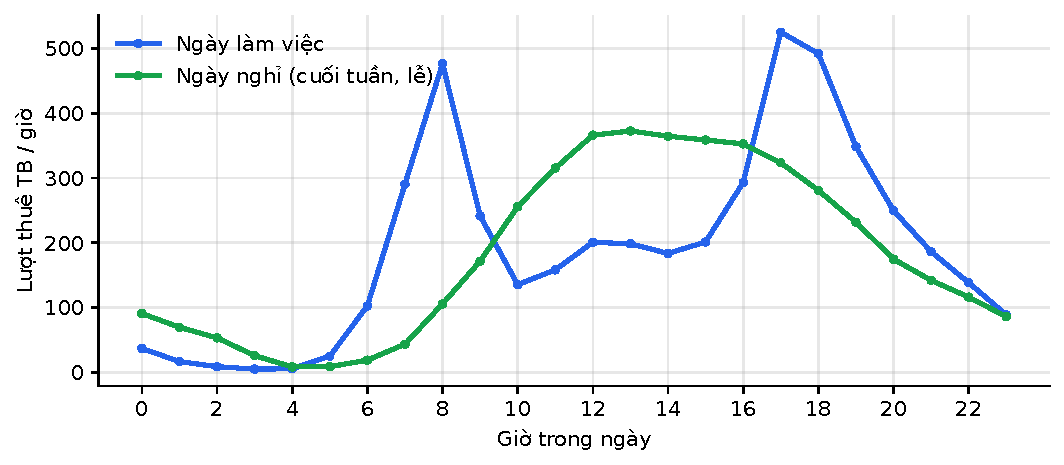
\includegraphics[width=0.95\textwidth]{figures/hourly_profile.pdf}
\caption{Lượt thuê trung bình theo giờ: ngày làm việc và ngày nghỉ}
\label{fig:hourly}
\end{figure}

\noindent\textbf{Q1.3 - Khác biệt giữa các ngày trong tuần.} Năm 2011 nhu cầu trung bình/giờ gần như đều giữa các thứ (137,6--147,6). Năm 2012 có khác biệt rõ hơn: thấp nhất Chủ nhật (210,0), cao nhất thứ Năm (249,5). Khác biệt lớn nhất nằm ở \textbf{thành phần người dùng} (Hình~\ref{fig:users}): người dùng vãng lai chiếm 31,6\% (Chủ nhật) và 32,2\% (thứ Bảy), nhưng chỉ 12--16\% vào các ngày trong tuần.

\begin{figure}[H]
\centering
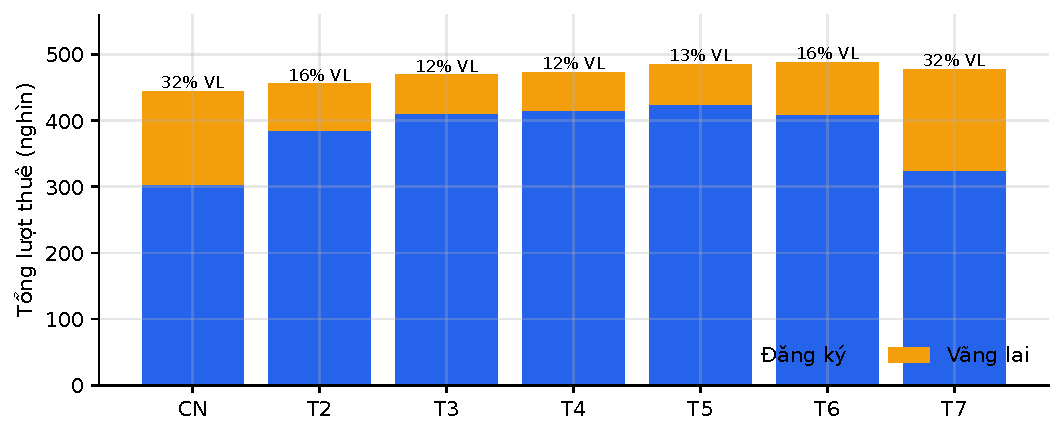
\includegraphics[width=0.92\textwidth]{figures/users_weekday.pdf}
\caption{Lượt thuê theo thứ trong tuần và tỷ lệ người dùng vãng lai (VL)}
\label{fig:users}
\end{figure}

\noindent\textbf{Q1.4 - Theo mùa và tháng.} Theo mùa (mã mùa của nguồn), mùa 3 (Fall) có tổng lượt thuê cao nhất (1.061.129), sau đó là Summer (918.589), Winter (841.613) và thấp nhất Spring (471.348) - lưu ý mùa ``Spring'' của nguồn ứng với khoảng 21/12 -- 20/3, tức thực tế là mùa đông lạnh nhất. Theo tháng (Hình~\ref{fig:monthly}), nhu cầu thấp nhất vào tháng 1, tăng dần đến đỉnh mùa hè - thu (2011: tháng 6, 199,3 lượt/giờ; 2012: tháng 9, 303,6 lượt/giờ) rồi giảm vào cuối năm. Đường 2012 nằm trên đường 2011 ở mọi tháng.

\begin{figure}[H]
\centering
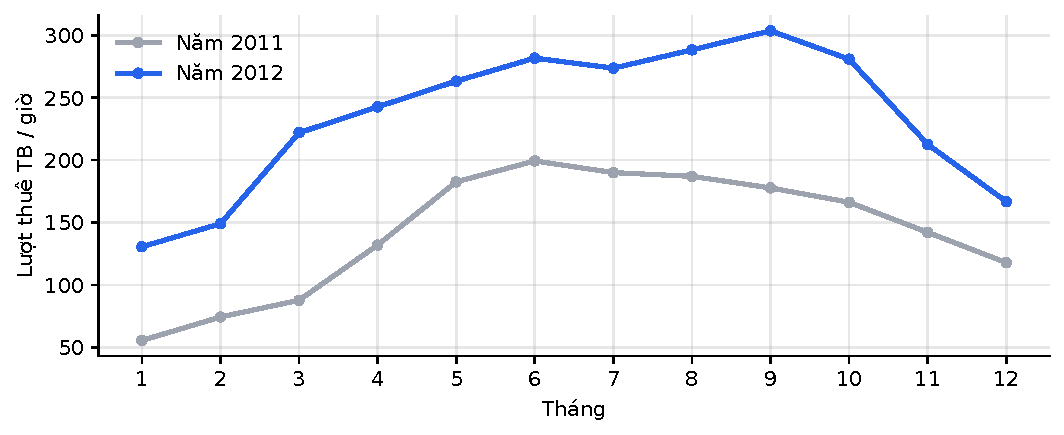
\includegraphics[width=0.92\textwidth]{figures/monthly_trend.pdf}
\caption{Lượt thuê trung bình/giờ theo tháng, so sánh hai năm}
\label{fig:monthly}
\end{figure}

\noindent\textbf{Q1.5 - Tỷ lệ người dùng.} Người dùng đăng ký chiếm \textbf{81,2\%} lượt thuê, vãng lai \textbf{18,8\%}. Tỷ lệ vãng lai thay đổi mạnh theo giờ: chỉ 5,5\% lúc 6h nhưng 29,8\% lúc 15h - người đăng ký chủ yếu dùng xe để đi làm, người vãng lai dùng xe để giải trí vào buổi chiều và cuối tuần.

\sect{Nhóm 2 - Ảnh hưởng của các yếu tố}

\noindent\textbf{Q2.1 - Thời tiết.} So với trời quang (204,9 lượt/giờ), trời sương mù làm nhu cầu giảm 14,5\% (175,2) và mưa/tuyết nhẹ làm giảm 45,5\% (111,6). Mức mưa lớn chỉ có 3 giờ quan sát (74,3) nên không đủ tin cậy để kết luận (Hình~\ref{fig:weather}, cột màu xám).

\begin{figure}[H]
\centering
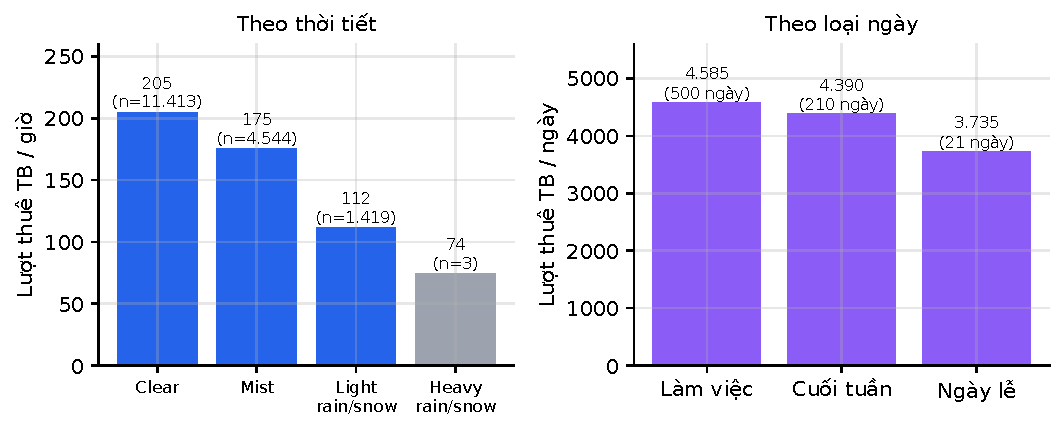
\includegraphics[width=0.95\textwidth]{figures/weather_daytype.pdf}
\caption{Lượt thuê trung bình theo thời tiết (theo giờ) và theo loại ngày (theo ngày)}
\label{fig:weather}
\end{figure}

\noindent\textbf{Q2.2 - Nhiệt độ và độ ẩm.} Nhiệt độ có tương quan \textbf{dương} với nhu cầu: $r = 0{,}41$ ở mức giờ và $r = 0{,}63$ ở mức ngày. Nhu cầu tăng đều từ 48,6 lượt/giờ (0--5$^\circ$C) lên 330,3 (30--35$^\circ$C), rồi giảm nhẹ khi trên 35$^\circ$C (318,5). Độ ẩm có tương quan \textbf{âm}: $r = -0{,}33$ ở mức giờ, nhu cầu giảm từ khoảng 300 lượt/giờ (độ ẩm 20--30\%) xuống 80,8 (90--100\%). Tuy nhiên ở mức ngày tương quan chỉ còn $r = -0{,}11$: phần lớn quan hệ theo giờ là do \textbf{biến gây nhiễu} giờ trong ngày (ban đêm vừa ẩm hơn vừa vắng khách). Phân tích độ ẩm dùng 17.357 giờ: 22 giờ độ ẩm 0\% (lỗi cảm biến, \code{humidity\_pct = NULL}) bị loại; khoảng 0--10\% chỉ còn 1 giờ nên được gắn cờ ít mẫu. Tương quan không đồng nghĩa nhân quả (Hình~\ref{fig:climate}).

\begin{figure}[H]
\centering
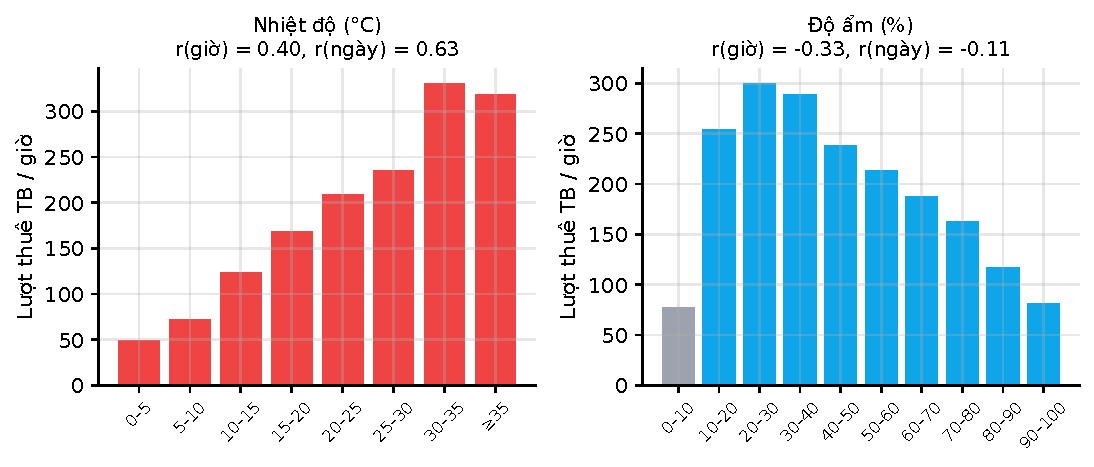
\includegraphics[width=0.95\textwidth]{figures/climate.pdf}
\caption{Lượt thuê trung bình/giờ theo khoảng nhiệt độ và độ ẩm (cột xám: dưới 30 giờ quan sát)}
\label{fig:climate}
\end{figure}

\noindent\textbf{Q2.3 - Ngày làm việc và ngày nghỉ.} Trung bình mỗi ngày làm việc có 4.585 lượt, cao hơn ngày nghỉ (4.330) khoảng 5,9\%; cụ thể cuối tuần 4.390 và ngày lễ 3.735 lượt/ngày. Khác biệt về tổng lượng không lớn, nhưng khác biệt về \textbf{phân bố trong ngày} rất lớn (Hình~\ref{fig:hourly}) - đây là lý do DSS phân loại theo từng giờ và từng loại ngày thay vì theo cả ngày.

\noindent\textbf{Q2.4 - Khung giờ cao trong ngày làm việc.} Theo khung giờ, ngày làm việc có trung bình cao nhất ở khung Chiều 16--19h (414,8 lượt/giờ) và Sáng 6--9h (277,9), thấp nhất khung Đêm (16,4). Theo từng giờ: 17h (525), 18h (492), 8h (477), 19h (348), 16h (293), 7h (291).

\sect{Nhóm 3 - Hỗ trợ ra quyết định}
Các câu hỏi nhóm 3 được trả lời bằng thành phần DSS (mục~\ref{sec:dss}):
\begin{itemize}
    \item \textbf{Q3.1 - Khung giờ ưu tiên}: ngày làm việc trời quang ưu tiên theo thứ tự 17h, 18h, 8h, 19h, 16h, 7h, 20h, 9h; ngày nghỉ ưu tiên 10--19h, cao nhất 12--13h.
    \item \textbf{Q3.2 - Mức nhu cầu của một giờ}: tra trực tiếp trên kế hoạch 24 giờ hoặc ma trận phân loại (Hình~\ref{fig:dss-matrix}); ví dụ 8h ngày làm việc mưa nhẹ vẫn là \High{} (263 lượt/giờ), 8h ngày nghỉ trời quang là \Med{} (112).
    \item \textbf{Q3.3 - Chuẩn bị nguồn lực cho khung giờ sắp tới}: chọn loại ngày và thời tiết dự báo, hệ thống trả về khuyến nghị cho từng giờ (Bảng~\ref{tab:rules}, \ref{tab:scenarios}).
    \item \textbf{Q3.4 - Cảnh báo}: hệ thống gộp các giờ Cao thành khung cảnh báo kèm giờ đỉnh và giờ phải chuẩn bị xong, ví dụ: ``Nhu cầu dự kiến CAO trong khung 16:00--20:59 (đỉnh 17h, TB 574 lượt/giờ). Hoàn tất chuẩn bị thêm xe và nhân sự trước 15:00.''
\end{itemize}

% ==================== CHƯƠNG 10 ====================
\newpage
\chap{Kiểm thử và đánh giá}\label{sec:eval}

\sect{Kiểm thử tự động}
Bộ kiểm thử dùng \code{pytest} và \code{FastAPI TestClient}, chạy bằng \code{python -m pytest tests -q}. Điểm chính: các kiểm thử không chỉ kiểm tra API ``chạy được'' mà \textbf{đối chiếu kết quả với dữ liệu nguồn} được tính độc lập bằng Pandas từ \code{hour.csv}. Kết quả lần chạy cuối: \textbf{40/40 kiểm thử đạt}.

\begin{table}[H]
\centering
\caption{Các bộ kiểm thử tự động}
\label{tab:tests}
\small
\begin{tabularx}{\textwidth}{|l|c|X|}
\hline
\textbf{Tệp} & \textbf{Số test} & \textbf{Nội dung kiểm tra} \\ \hline
\code{test\_etl.py} & 9 & (Không cần CSDL) bước Transform trên dữ liệu nguồn thật: số dòng các bảng; tổng lượt thuê được bảo toàn; khóa ngoại của fact tồn tại trong chiều, không trùng (ngày, giờ); \code{hours\_recorded} (ngày 29/10/2012 chỉ có 1 giờ); 22 dòng \code{hum = 0} thành NULL; thứ trong tuần khớp nguồn; từ chối dữ liệu ngoài miền và lịch không nhất quán; loại dòng vi phạm tổng \\ \hline
\code{test\_api.py} & 8 & KPI khớp tổng nguồn; roll-up nhất quán (tổng các quý = tổng năm); drill-down tới ngày, giờ; slice/dice thu hẹp đúng; tổng pivot = tổng toàn bộ; lỗi tham số trả về 422; chuỗi SQL injection vô hại \\ \hline
\code{test\_climate.py} & 4 & Số giờ, trung bình mỗi khoảng nhiệt độ và độ ẩm khớp Pandas; tổng số giờ các khoảng nhiệt độ = 17.379, độ ẩm = 17.357 (loại 22 giờ NULL, không bị dồn vào khoảng 90--100\%); cờ ít mẫu đúng; hệ số tương quan khớp Pandas; bộ lọc có hiệu lực \\ \hline
\code{test\_dss\_engine.py} & 11 & (Không cần CSDL) biên phân loại (bằng ngưỡng là Trung bình); ngưỡng không hợp lệ bị từ chối; mỗi mức có khuyến nghị; kế hoạch đủ 24 giờ, mỗi giờ đúng một mức; danh sách ưu tiên giảm dần; gộp khung cảnh báo, giờ chuẩn bị qua nửa đêm; xử lý nhóm thiếu/ít dữ liệu; biên phân nhóm khách (1,5 và 0,75 lần tỷ lệ chung); khung cảnh báo mang tỷ lệ vãng lai và khuyến nghị nhóm khách, không làm đổi mức nhu cầu; kế hoạch theo một hoặc nhiều thứ (nhãn, bỏ trùng, sắp T2 $\rightarrow$ CN, suy ra loại ngày, từ chối thứ không hợp lệ) \\ \hline
\code{test\_dss\_api.py} & 8 & Ngưỡng khớp phân vị tính bằng Pandas; mỗi mức chiếm 30--37\% giờ quan sát; trung bình nhóm khớp nguồn; giờ 8h và 17h ngày làm việc được cảnh báo; ngưỡng thay đổi theo kỳ lịch sử; bộ lọc ngoài kỳ không ảnh hưởng DSS; mức thời tiết 4 bị gắn cờ; lỗi tham số trả về 422; tỷ lệ vãng lai từng giờ khớp Pandas; cao điểm ngày làm việc là ``chủ yếu đăng ký'' và ngày nghỉ là ``nhiều vãng lai''; kế hoạch theo thứ (thứ hai, thứ sáu, thứ bảy) khớp trung bình nguồn, chiều thứ sáu có khung cao từ 12h, thứ không hợp lệ trả về 422; nhiều thứ (T2 + T3) khớp nguồn, chọn đủ T2--T6 trùng nhóm ngày làm việc \\ \hline
\end{tabularx}
\end{table}
Ngoài ra, quy trình ETL tự đối chiếu 13 tiêu chí với cả hai tệp nguồn (Bảng~\ref{tab:etl-validate}), và các truy vấn trong \code{sql/03\_olap\_queries.sql}, \code{sql/04\_dss\_queries.sql} đã được chạy thử trên kho.

\sect{Hiệu năng}
Thời gian phản hồi được đo bằng cách gọi mỗi endpoint 10 lần trên máy cá nhân (Windows 11, PostgreSQL cục bộ). Số đo bao gồm cả việc mở kết nối CSDL mới cho mỗi yêu cầu.

\begin{table}[H]
\centering
\caption{Thời gian phản hồi của API (ms)}
\label{tab:perf}
\begin{tabular}{|l|r|r|}
\hline
\textbf{Yêu cầu} & \textbf{Trung vị} & \textbf{Lớn nhất} \\ \hline
\code{/api/kpis} (toàn bộ dữ liệu) & 77 & 197 \\ \hline
\code{/api/kpis} (dice: 2012, hè+thu, ngày làm việc) & 57 & 183 \\ \hline
\code{/api/olap/drill} (tháng của 2012) & 54 & 185 \\ \hline
\code{/api/olap/pivot} (tháng $\times$ thời tiết) & 54 & 155 \\ \hline
\code{/api/hourly} & 52 & 176 \\ \hline
\code{/api/climate} & 105 & 227 \\ \hline
\code{/api/dss/plan} & 68 & 88 \\ \hline
\code{/api/dss/matrix} & 71 & 175 \\ \hline
\end{tabular}
\end{table}
Mọi yêu cầu đều dưới 0,25 giây, đáp ứng NFR03 (mục tiêu dưới 1 giây).

\sect{Đánh giá mức độ đáp ứng yêu cầu}
\begin{table}[H]
\centering
\caption{Đánh giá yêu cầu chức năng}
\label{tab:fr-eval}
\small
\begin{tabularx}{\textwidth}{|c|c|X|}
\hline
\textbf{Mã} & \textbf{Mức đáp ứng} & \textbf{Bằng chứng} \\ \hline
FR01 & Đạt & \code{extract.py} đọc hai tệp CSV \\ \hline
FR02 & Đạt & \code{clean()}: thiếu, trùng, kiểu, miền giá trị, ràng buộc tổng (mục~\ref{sec:etl}) \\ \hline
FR03 & Đạt & Star Schema 1 fact, 3 dimension (Hình~\ref{fig:star}) \\ \hline
FR04 & Đạt & ETL một lệnh, giao dịch, 13/13 phép đối chiếu PASS \\ \hline
FR05 & Đạt & Drill-down năm $\rightarrow$ giờ, tổng hợp theo mùa, tháng, thứ \\ \hline
FR06 & Đạt & Thời tiết, nhiệt độ, độ ẩm, loại ngày, nhóm người dùng \\ \hline
FR07 & Đạt & Roll-up, drill-down, slice, dice, pivot (SQL và giao diện) \\ \hline
FR08 & Đạt & 8 KPI, biểu đồ drill-down, 5 biểu đồ phân tích, bảng pivot, bộ lọc dùng chung \\ \hline
FR09 & Đạt & Phân loại 3 mức theo ngưỡng phân vị khảo sát từ dữ liệu \\ \hline
FR10 & Đạt & Khuyến nghị theo mức, khung cảnh báo, danh sách ưu tiên \\ \hline
\end{tabularx}
\end{table}

\begin{table}[H]
\centering
\caption{Đánh giá yêu cầu phi chức năng}
\label{tab:nfr-eval}
\small
\begin{tabularx}{\textwidth}{|c|c|X|}
\hline
\textbf{Mã} & \textbf{Mức đáp ứng} & \textbf{Nhận xét} \\ \hline
NFR01 & Đạt & Đối chiếu ETL và kiểm thử khớp nguồn đến từng ngày, từng nhóm \\ \hline
NFR02 & Đạt & PK, FK, CHECK, UNIQUE; 0 dòng mồ côi \\ \hline
NFR03 & Đạt & Mọi yêu cầu dưới 0,25 giây (Bảng~\ref{tab:perf}) \\ \hline
NFR04 & Đạt một phần & Thêm chiều, thêm thuộc tính dễ dàng nhờ Star Schema và view; nhưng ETL hiện nạp lại toàn bộ, chưa nạp tăng dần \\ \hline
NFR05 & Đạt & ETL, SQL, API, DSS, giao diện là các module riêng \\ \hline
NFR06 & Đạt & Bộ lọc chip áp dụng cho mọi biểu đồ, chú thích độ tin cậy; chưa khảo sát người dùng thật \\ \hline
NFR07 & Đạt & Mô hình DSS kiểm thử và bước Transform kiểm thử không cần CSDL; 40 kiểm thử tự động \\ \hline
\end{tabularx}
\end{table}

\sect{Đánh giá thành phần DSS}
\textbf{Điểm mạnh}: mô hình minh bạch, giải thích được (người vận hành hiểu vì sao một giờ là ``Cao''); ngưỡng xuất phát từ khảo sát phân phối và có thể điều chỉnh; kết quả ổn định khi thay đổi ngưỡng và kỳ lịch sử (mục~\ref{sec:dss-sensitivity}); trung thực về độ tin cậy khi dữ liệu thưa; tích hợp trực tiếp với kho dữ liệu nên tự cập nhật khi nạp dữ liệu mới.

\textbf{Hạn chế}: mô hình là mô hình tra cứu theo nhóm (trung bình lịch sử), chưa phải mô hình dự báo, nên không phản ánh xu hướng tăng trưởng trong kỳ và không xét đồng thời nhiệt độ, độ ẩm; chưa được đánh giá bằng dữ liệu ngoài mẫu (ví dụ dùng 2011 xác định mức, kiểm tra trên 2012); khuyến nghị dừng ở mức độ, chưa có số xe cụ thể.

% ==================== CHƯƠNG 11 ====================
\newpage
\chap{Hạn chế và hướng phát triển}\label{sec:limits}

\sect{Hạn chế}
\begin{enumerate}
    \item \textbf{Dữ liệu}: chỉ có giai đoạn 2011--2012, quy mô vừa phải (17.379 dòng sự kiện), mức tổng toàn hệ thống; không có vị trí trạm, số xe sẵn sàng, lịch sử điều chuyển xe. Vì vậy DSS chỉ khuyến nghị mức độ chuẩn bị, chưa giải được bài toán điều phối giữa các trạm.
    \item \textbf{Chất lượng dữ liệu}: 165 giờ thiếu bản ghi (76 ngày không đủ 24 giờ), 22 giờ độ ẩm bằng 0, 12,5\% số giờ có tốc độ gió bằng 0, mức thời tiết 4 chỉ có 3 giờ; mã mùa của nguồn lệch so với mùa theo cảm nhận (``Spring'' thực chất là mùa đông). Các vấn đề này đã được ghi nhận và gắn cờ, nhưng không sửa được từ phía nguồn.
    \item \textbf{Nạp dữ liệu}: ETL nạp lại toàn bộ (phù hợp dữ liệu tĩnh), chưa có cơ chế nạp tăng dần, chưa có lịch chạy tự động.
    \item \textbf{Mô hình DSS}: dựa trên trung bình lịch sử theo nhóm; chưa xét đồng thời nhiều biến liên tục (nhiệt độ, độ ẩm, gió). Kiểm định ngoài mẫu (mục~\ref{sec:dss-backtest}) cho thấy mô hình tĩnh bỏ sót nhiều giờ cao điểm khi nhu cầu tăng (recall mức Cao 58,5\%), và hiệu chỉnh mức theo sai số gần nhất khắc phục phần lớn (recall 90,0\%). Hạn chế còn lại: kiểm định dùng thời tiết thực tế của năm 2012 nên kết quả vận hành sẽ thấp hơn, và mới chỉ có một năm kiểm thử.
    \item \textbf{Hệ thống}: chưa có xác thực người dùng, chưa triển khai lên máy chủ; tương quan nhiệt độ, độ ẩm chưa kiểm soát đầy đủ biến gây nhiễu.
\end{enumerate}

\sect{Hướng phát triển}
\begin{enumerate}
    \item \textbf{Mở rộng dữ liệu}: dùng dữ liệu chuyến đi chi tiết mà Capital Bikeshare công bố (có trạm đi, trạm đến, thời lượng), bổ sung chiều \textbf{Trạm} (áp dụng SCD loại 2 cho thay đổi sức chứa, vị trí) và bảng sự kiện \textbf{tồn xe theo trạm}; khi đó DSS có thể tính số xe cần điều chuyển giữa các trạm (bài toán tối ưu, ví dụ quy hoạch tuyến tính).
    \item \textbf{Nạp tăng dần}: ETL theo lô hằng ngày, dùng khóa nghiệp vụ \code{(date\_key, hour\_key)} để upsert; phân vùng bảng sự kiện theo năm khi dữ liệu lớn; lập lịch chạy tự động.
    \item \textbf{Mô hình dự báo}: thay mô hình tra cứu bằng mô hình hồi quy hoặc học máy (ví dụ gradient boosting) nhận đầu vào giờ, loại ngày, dự báo thời tiết, nhiệt độ, xu hướng; phân loại mức dựa trên khoảng dự báo thay vì chỉ trung bình. Khung kiểm định ngoài mẫu đã có (mục~\ref{sec:dss-backtest}: huấn luyện 2011, kiểm tra 2012, cùng các chỉ số độ chính xác, recall mức Cao, tỷ lệ thiếu/dư chuẩn bị, MAE), nên có thể dùng lại để so sánh mô hình mới với mô hình hiện tại trên cùng thước đo.
    \item \textbf{Tích hợp dự báo thời tiết} qua API để tự động lập kế hoạch cho ngày mai và gửi cảnh báo (email, tin nhắn) cho người vận hành.
    \item \textbf{Hệ thống}: thêm xác thực, phân quyền; đóng gói Docker và triển khai; bổ sung bộ đệm (cache) cho các truy vấn tổng hợp hoặc materialized view khi dữ liệu lớn.
\end{enumerate}

% ==================== CHƯƠNG 12 ====================
\newpage
\chap{Thiết lập và khởi chạy dự án}\label{sec:setup}

\sect{Yêu cầu môi trường}
Python 3.10 trở lên, Node.js 18 trở lên, PostgreSQL 14 trở lên. Mã nguồn: \repoURL.

\sect{Các bước cài đặt}
\begin{lstlisting}[language=bash, caption={Cài đặt và nạp kho dữ liệu}]
# 1. Cai thu vien Python
pip install -r requirements.txt
# 2. Cau hinh ket noi: sao chep .env.example thanh .env, dien PGPASSWORD
#    (va PGHOST/PGPORT/PGUSER neu khac mac dinh)
cp .env.example .env
# 3. Tao database bike_dw (pgAdmin hoac psql), mot lan
createdb -U postgres bike_dw
# 4. Chay ETL: tao schema dw, nap du lieu, doi chieu -> docs/validation_report.md
python src/etl/run_etl.py
\end{lstlisting}

\begin{lstlisting}[language=bash, caption={Chạy API và dashboard (hai cửa sổ terminal)}]
# Terminal 1 - API (cong 8000), chay tu thu muc goc repo
python -m uvicorn --app-dir src api.main:app --port 8000
# Terminal 2 - Dashboard (cong 5173)
cd src/dashboard
npm install          # chi lan dau
npm run dev          # mo http://localhost:5173
\end{lstlisting}
Tài liệu API tự sinh tại \code{http://localhost:8000/docs}.

\begin{lstlisting}[language=bash, caption={Kiểm thử và sinh lại hình cho báo cáo}]
pip install -r requirements-dev.txt
python -m pytest tests -q                  # can DB da nap ETL
python report/scripts/make_figures.py      # sinh report/figures/*.pdf
\end{lstlisting}

% ==================== CHƯƠNG 13 ====================
\newpage
\chap{Kết luận}\label{sec:conclusion}
Bài tập lớn đã xây dựng hoàn chỉnh hệ thống \textbf{Bike Sharing DW \& DSS} đáp ứng các mục tiêu của quy định:
\begin{itemize}
    \item \textbf{Phân tích yêu cầu}: xác định bài toán chuẩn bị nguồn lực theo giờ của đơn vị vận hành, 13 câu hỏi nghiệp vụ, 10 yêu cầu chức năng, 7 yêu cầu phi chức năng và 8 KPI.
    \item \textbf{Thiết kế DW}: Star Schema độ hạt theo giờ với 3 chiều, các vấn đề thiết kế được phân tích và giải quyết có lý do; quy trình ETL làm sạch, nạp trong giao dịch và đối chiếu 13/13 tiêu chí với nguồn; các vấn đề chất lượng (giờ thiếu, độ ẩm 0\%) được đánh dấu ngay trong kho.
    \item \textbf{Hiện thực}: PostgreSQL, truy vấn OLAP đủ năm phép toán, REST API 12 endpoint phân tích, dashboard React với bộ lọc dùng chung, KPI, drill-down, pivot.
    \item \textbf{DSS}: mô hình phân loại nhu cầu ba mức với ngưỡng khảo sát từ phân phối dữ liệu, khuyến nghị, cảnh báo theo khung giờ, danh sách ưu tiên, phân tích độ nhạy và đánh giá độ tin cậy.
    \item \textbf{Đánh giá}: 33 kiểm thử tự động đối chiếu với nguồn, thời gian phản hồi dưới 0,25 giây; hạn chế và hướng phát triển được nêu rõ.
\end{itemize}
Kết quả phân tích cho thấy những quy luật có giá trị vận hành: hệ thống tăng trưởng 64,9\% từ 2011 sang 2012; ngày làm việc có hai khung cao điểm 7--9h và 16--20h, ngày nghỉ có một khung dài 10--19h; mưa nhẹ làm giảm gần một nửa nhu cầu nhưng nhu cầu đi làm giờ cao điểm vẫn ở mức Cao; nhiệt độ có ảnh hưởng dương rõ rệt. Các khung giờ ưu tiên mà DSS đưa ra ổn định khi thay đổi ngưỡng và kỳ lịch sử.

Qua đề tài, nhóm đã vận dụng được chuỗi kiến thức của môn học - từ khái niệm kho dữ liệu, quy trình thiết kế đa chiều, ETL, OLAP đến mô hình hóa và xây dựng hệ hỗ trợ quyết định - vào một bài toán thực tế của giao thông đô thị, đồng thời thấy rõ vai trò của kho dữ liệu như nền tảng dữ liệu tin cậy cho DSS.


% ==================== TÀI LIỆU THAM KHẢO ====================
\newpage
\renewcommand{\refname}{Tài liệu tham khảo}
\begin{thebibliography}{99}
  \bibitem{inmon} W. H. Inmon, \textit{Building the Data Warehouse}, 4th ed. Wiley, 2005.
  \bibitem{kimball} R. Kimball, M. Ross, \textit{The Data Warehouse Toolkit}, 3rd ed. Wiley, 2013.
  \bibitem{turban} E. Turban, J. E. Aronson, T.-P. Liang, \textit{Decision Support Systems and Intelligent Systems}, 7th ed. Prentice-Hall, 2005.
  \bibitem{elmasri} R. Elmasri, S. B. Navathe, \textit{Fundamentals of Database Systems}, 7th ed. Addison-Wesley, 2016.
  \bibitem{sharda} R. Sharda, D. Delen, E. Turban, \textit{Analytics, Data Science, \& Artificial Intelligence: Systems for Decision Support}, 7th ed. Pearson, 2020.
  \bibitem{han} J. Han, M. Kamber, J. Pei, \textit{Data Mining: Concepts and Techniques}, 3rd ed. Morgan Kaufmann, 2012.
  \bibitem{burstein} F. Burstein, C. W. Holsapple, \textit{Handbook on Decision Support Systems}. Springer, 2008.
  \bibitem{quang} Trần Minh Quang et al., \textit{Cơ sở dữ liệu: khái niệm, phương pháp, và kỹ thuật phân tích thiết kế}. NXB ĐHQG-HCM, 2025.
  \bibitem{simon} H. A. Simon, \textit{The New Science of Management Decision}. Harper \& Row, 1960.
  \bibitem{fanaee} H. Fanaee-T, J. Gama, ``Event labeling combining ensemble detectors and background knowledge,'' \textit{Progress in Artificial Intelligence}, vol. 2, pp. 113--127, 2014.
  \bibitem{uci} UCI Machine Learning Repository, \textit{Bike Sharing Dataset}, \url{https://archive.ics.uci.edu/dataset/275/bike+sharing+dataset}
  \bibitem{postgres} PostgreSQL Global Development Group, \textit{PostgreSQL Documentation: Aggregate Functions (GROUPING SETS, ROLLUP, percentile\_cont)}, \url{https://www.postgresql.org/docs/}
  \bibitem{fastapi} FastAPI Documentation, \url{https://fastapi.tiangolo.com/}
  \bibitem{react} React Documentation, \url{https://react.dev/}
  \bibitem{recharts} Recharts - A composable charting library built on React components, \url{https://recharts.org/}
\end{thebibliography}

\end{document}
